\documentclass[11pt,a5paper]{book}

\usepackage[utf8]{inputenc}
\usepackage[T1]{fontenc}
\usepackage{libertine}
\usepackage{ccicons}
\usepackage{marvosym}
\usepackage{textcomp}
\usepackage[spanish]{babel}
\addto{\captionsspanish}{
    \renewcommand{\contentsname}{Índice}
    \renewcommand{\prefacename}{Prólogo}
    \renewcommand{\chaptername}{}
    \renewcommand{\appendixname}{Anual}
}

\newcommand{\titlename}{Los Caídos}
\newcommand{\subtitlename}{Volúmen II}
\newcommand{\authorname}{Magnus Dagon}
\newcommand{\editorname}{Xoan Sampaiño}
\newcommand{\editorlogo}{\setlength{\fboxrule}{1pt}\fbox{\textbf{\fontfamily{ppl}\selectfont XS}}}
\newcommand{\coverauthorname}{Pablo Vaquero}
%\newcommand{\prefaceauthorname}{Jose A.~Carrasco}

\title{\textbf{\Huge\titlename}\\\textsc{\small\subtitlename}\setcounter{page}{3}}
\author{\textit{\authorname}}
\date{}

\usepackage{graphicx}
\usepackage[activate={true,nocompatibility},final]{microtype}

\usepackage{eso-pic}
\usepackage[top=1cm,bottom=1cm,outer=1.5cm,inner=2cm,includehead,includefoot]{geometry}
\usepackage[a4,cam,center]{crop}
\usepackage{fancyhdr}
\setlength{\headheight}{14pt}
\renewcommand{\headrulewidth}{0pt}
\lhead[\fancyplain{}{\thepage}]{\fancyplain{}{\footnotesize\nouppercase\leftmark}}
\rhead[\fancyplain{}{\footnotesize\titlename. \subtitlename}]{\fancyplain{}{\thepage}}
\cfoot{}
\pagestyle{fancy}
\usepackage{multicol}
\setlength{\columnsep}{1cm}
\usepackage{tocloft}
\renewcommand{\cftchapaftersnum}{\cftdot}
\renewcommand{\cftchapleader}{\cftdotfill{\cftdotsep}}
\usepackage[clearempty]{titlesec}
\usepackage[titletoc]{appendix}

\makeatletter
\def\vhrulefill#1{\leavevmode\leaders\hrule\@height#1\hfill\kern\z@}
\makeatother

\newcommand{\parbreak}{\bigskip}
\newcommand{\fancyparbreak}{\bigskip\centerline{\libertineGlyph{uniE007}$\ast$\libertineGlyph{uniE007}}\bigskip}

\newcommand{\typo}[2]{\textcolor{red}{#1}\marginpar{\footnotesize\textcolor{green}{#2}}}

\usepackage{hyperref,hyperxmp}
\hypersetup{
    pdftitle={\titlename. \ \subtitlename},
    pdfauthor={\authorname},
    pdfcopyright={\copyright\ 2010-2011, \authorname\012%
        \copyright\ 2011, de la edición, \editorname\012\012%
        Se otorga el permiso para copiar, publicar y/o distribuir libremente esta obra y/u obras derivadas de esta obra, ya sea total o parcialmente, por cualquier medio y con cualquier propósito sin ánimo de lucro, siempre y cuando esta nota se mantenga.
    },
    pdflicenseurl={http://creativecommons.org/licenses/by-nc-sa/3.0/es/},
    bookmarksnumbered={true}
}

\begin{document}
\pagecolor{black}
\thispagestyle{empty}
\pagenumbering{alph}
\AddToShipoutPicture*{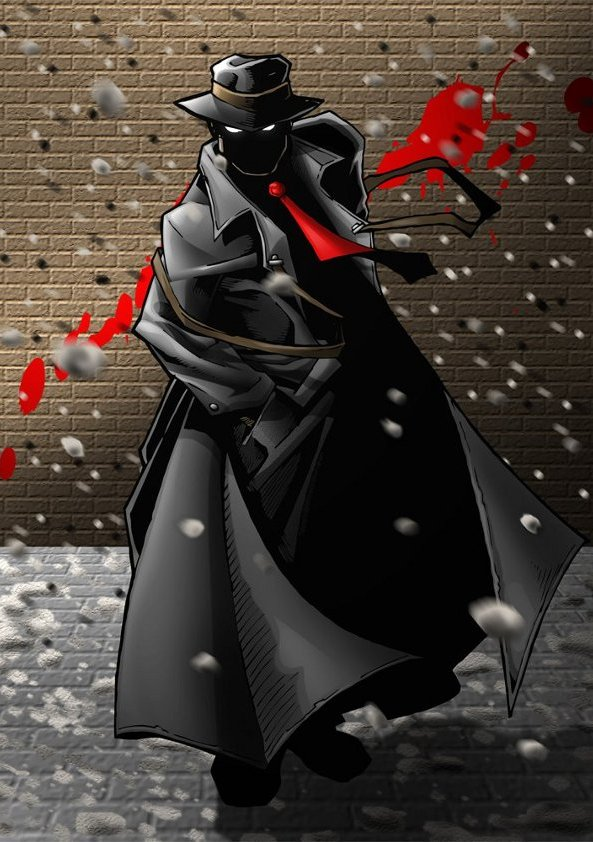
\includegraphics[width=\paperwidth,height=\paperheight]{images/cover}}
\begin{center}
    \color{white}\vspace*{\stretch{1}}

    \textbf{\fontsize{60}{72}\selectfont\itshape\thetitle}\vspace{1.5\baselineskip}

    \rule{0.5\textwidth}{3pt}\vspace{0.5\baselineskip}

    \textbf{\LARGE\theauthor}\vspace*{\stretch{1}}

    \large\theeditorial
\end{center}

\endinput

\newpage\pagecolor{white}

\frontmatter
\thispagestyle{empty}
\hbox{}\newpage
\thispagestyle{empty}
\vspace*{\stretch{1}}\noindent
\textbf{\titlename}\\
\authorname

\footnotesize

\bigskip\bigskip\noindent
\textbf{\copyright\ 2010--2011, \authorname}\\
\textbf{\copyright\ 2011, de la edición, \editorname}\\
Se otorga el permiso para copiar, publicar y/o distribuir libremente esta obra y/u obras derivadas de esta obra, ya sea total o parcialmente, por cualquier medio y con cualquier propósito sin ánimo de lucro, siempre y cuando esta nota se mantenga.\\
{\fontencoding{OT1}\fontfamily{cmr}\selectfont\url{http://creativecommons.org/licenses/by-nc-sa/3.0/es/}}

\normalsize

\noindent\ccbyncsaeu

\footnotesize

\bigskip\noindent
\textbf{Edición:} \editorname\\
Realizada íntegramente con \emph{software libre}, mediante el procesador \LaTeXe\\
\Letter\ {\fontencoding{OT1}\fontfamily{cmr}\selectfont\href{mailto:xoansampainho@gmail.com}{\nolinkurl{xoansampainho@gmail.com}}}\\
\Telefon\ \href{tel:+34620194971}{+34 620194971}

\bigskip\noindent
Impreso en la Red. \emph{Printed in Internet}

\normalsize

\endinput


\maketitle

\cleardoublepage
\raggedcolumns
\tableofcontents
\flushcolumns

\mainmatter
\setcounter{chapter}{24}
\addtocontents{toc}{\protect\vspace{0.5\cftbeforechapskip}\protect\begin{multicols}{2}}
\chapter{Plan oculto}
Muchas preguntas ya tenían respuesta. Pero al mismo tiempo, nuevas incógnitas salían a la luz. Misterios que hacían tambalearse la estructura misma de la organización y arrojaban nuevas y sorprendentes pistas sobre su origen.
Y gran parte de esas respuestas estaban en manos del que había sido hasta ese momento su enemigo parapetado en el anonimato\dots

\fancyparbreak
Sam Grove le dijo que no se lo creería cuando lo supiera. No se hacía una idea de cuánta razón tenía.

El Juez Nitram y Starr Miles, aliados. Amigos. O al menos, algo muy similar. Las circunstancias concretas de esa relación eran aún desconocidas para ellos, pero sin duda distaban mucho de ser de naturaleza meramente casual. La justicia había movido los actos de aquellos dos hombres desde antes que él mismo pusiera los pies sobre una nave espacial. Eran perros viejos en un mundo más viejo aún.

Y ahora el pasado regresaba para ponerlo todo a prueba. Establecer la duda, la incertidumbre sobre en qué han estado basando realmente todo aquello que han construido. Quién era realmente Starr Miles. Él mismo decía que el pasado no importaba, sólo el presente. Pero lo que por aquel entonces era el presente ya se había convertido en el pasado para todos ellos.

Ya habría tiempo de indagar en detalle sobre lo que acababa de salir a la luz, por otro lado. Era el momento de la acción. De atacar con fuerza, rapidez y contundencia.

Como Echo había anticipado, los suyos no habían perdido el tiempo en su ausencia. Ya tenían los datos de la inmensa mansión en la que Nitram se había retirado, un lugar que al parecer ocupaba de manera habitual para alejarse de las cámaras que atormentaban a otros jueces y otras personalidades públicas. No había cifras exactas, pero la mansión podía estar fácilmente vigilada por treinta o cuarenta guardaespaldas, y eso sin contar con torretas de seguridad en pasillos y puntos muertos.

El concierto de The Jammers no había empezado aún, además. Grove estaba allí, infiltrado entre el público, esperando dar la buena noticia de que las comunicaciones se habían restablecido de la manera más clara posible: usando como prueba el propio mensaje enviado. Su escuadrón también estaría por los alrededores, de modo que se pudiera restablecer la normalidad en la medida de lo posible.

Según los datos de Razorclaw habían sucumbido veinticuatro hombres en las calles desde el comienzo de la vendetta. Diez habían sido descubiertos por cazarrecompensas y obligados a fingir ser imitadores, cinco habían sacrificado su puesto para llamar la atención de manera voluntaria y añadir confusión a los casos anteriores, cinco habían sido heridos de gravedad y dos parejas habían muerto, una de ellas a causa de las letales heridas y otra al autoinmolarse para proteger el secreto.

En total, la organización había perdido a la cuarta parte de sus componentes, pero tendrían que aprender a surgir de las cenizas. Lo primero de todo sería que no se ampliaría la formación. Casi todos los que habían muerto eran novatos, y no se perdonaría que algo así pudiera pasar de nuevo. Aquella experiencia le había enseñado que, si bien eran un equipo, cada hombre tenía que estar sobradamente preparado para actuar como si estuviera solo frente a todas las adversidades existentes en el mundo.

De todos modos, Los Caídos no podrían ser de mucha ayuda en el asalto al interior de la casa. Dado que las comunicaciones aún no se habían restablecido, lo que harían sería asegurar el exterior y los alrededores y dejar la parte de la infiltración a él y los cazarrecompensas, más que ansiosos por llegar hasta el epicentro del asunto.

Cuando se reunió con ellos comprobó que, pese a que Krexon se había escabullido, no habían estado perdiendo el tiempo precisamente. El socio de Dobleseis, Códec, tenía un buen arsenal que no habían desaprovechado en lo más mínimo, y pudo comprobar cómo estaban armados hasta los dientes con toda clase de lanzarrayos, gran parte de potencia no letal, pero muchos otros, pensados para las defensas automáticas, más que demoledores.

Dobleseis, sin embargo, apenas cogió armas. Estaba extasiado con su juguete nuevo, y planeaba toda clase de maniobras que realizar a dos manos con aquellos revólveres multiusos. Scream no quería ni pensar qué hubiera podido hacer Silenciador en su momento si hubiera tenido la capacidad del cazarrecompensas para poder dividir su concentración y puntería con simétrica eficacia.

Los cazarrecompensas, dentro del hecho de que eran tipos que actuaban por separado, se habían logrado compenetrar bastante bien. La planificación fue sencilla, rápida y ágil. No había sitio a las sutilezas en aquella ocasión. Además, la improvisación sería una parte esencial del ataque. Gracias a Saw, que había estado dentro de aquella casa en el pasado, cuando trabajaba para Gorgon, conocían el emplazamiento de los lugares más importantes de la misma, pero la disposición, en mayor o menor medida, podía haber cambiado.

La mansión disponía de tres plantas y estaba realizada en estilo precolonial, con una fachada adornada con complicadas escalinatas y columnas de orden corintio. Los ventanales poseían amplios dinteles, pero el blindaje de los cristales era muy resistente y difícil de atravesar. El techo permanecía también bajo vigilancia, y en términos globales el lugar apenas tenía entradas secundarias de tipo alguno, pues el garaje era subterráneo y se accedía desde un pasadizo situado muchos metros atrás. En su momento, de hecho, se intentó conectar una de las entradas del Aquerón con el interior de la mansión, pero resultó a todas luces imposible, si bien Scream no dudaba que la cantidad de pasillos secretos que debía poseer aquel lugar sin duda sería más que considerable dada su importancia política.

De todos modos, aunque no hubiera una entrada, no hubo problemas al respecto. Repulsor no tardó en fabricar una, tratando de calibrar al máximo el disparo para así no suponer un peso muerto una vez lo hubiera generado.

Los primeros en pasar fueron Dobleseis, Silencio y el propio Scream. Barrera cubriría a Repulsor, y Batería estaba al cargo de hacer que se recuperara cuanto antes, así como recargar de nuevo su equipo al completo. Fue por ello que obviamente se quedaron atrás en comparación con sus más veloces compañeros, que salieron disparados escaleras arriba para ganar una planta antes de que la movilización y la confusión les obligaran a pelear por cada palmo que recorrieran hacia la estancia principal, donde suponían que estaría Nitram, tal vez incluso esperándoles.

Las primeras defensas se cruzaron en el camino de los tres furtivos, y Dobleseis las despachó de un par de tiros sin dejarlas siquiera realinearse. Por desgracia la cosa empezó a ponerse al rojo vivo, y no tardaron en encontrarse con cinco hombres que les cortaban el paso. La batería de disparos fue encarnizada, pero uno por uno lograron derribarles, derrotando Scream a uno de ellos, Dobleseis a tres y Silencio al último, una vez logró colocarse a su espalda.

~---Perfecto, mudito ~---fue la única respuesta de Dobleseis. Silencio se acercó de nuevo a ellos, su actitud tranquila y pausada, evaluando la situación. Sin embargo de repente, sin previo aviso, apartó a Dobleseis de un golpe y recibió una descarga de una de las defensas automáticas abatidas, que había disparado con parte de energía residual que había logrado acumular.

El disparo no era fatal, pero el disparado estaba muy malherido. Dobleseis se quedó mirando, sin saber qué decir. Era la primera vez desde que era cazarrecompensas que alguien recibía de manera voluntaria un tiro en su lugar. Como única respuesta, frió la torreta con un disparo de sobrada potencia procedente de una de las antiguas armas del peor enemigo de Reflector.

Silencio les miró y les hizo un gesto para que continuaran.

~---¿Estarás bien? ~---preguntó Scream.

Escucharon ruido de disparos al fondo, y supieron que se trataba de sus compañeros rezagados. Silencio se limitó a hacer un gesto con la mano abierta para que se marcharan. No había que ser ningún lince para deducir que se ocultaría hasta que ellos alcanzaran su posición.

~---De acuerdo, seguiremos entonces.

Dobleseis y Scream prosiguieron a lo largo del pasillo, y si bien se encontraron con otros guardaespaldas por el camino, quedó claro que el grueso de la artillería ya había sido lanzado ya, algo más lógico que ir aumentando de manera escalonada la dificultad de los oponentes a medida que llegaban a su objetivo. Las defensas no supusieron problemas tampoco, aunque habían recalibrado su puntería en función de los movimientos de sus blancos y resultaba más complicado esquivar sus disparos, sobre todo para Scream, que confiaba más en engañarlas con sus dispositivos y hacer que sus rastreos de imagen, calor y cinética se confundieran para dispararse entre ellas.

~---Ingenioso ~---se limitó a decir Dobleseis al tiempo que recargaba sus cuatro lanzarrayos, con sus respectivas bocas humeantes y rojizas.

Ante ellos se alzaba la puerta de doble batiente que les separaba del despacho en el que sin duda se hallaba el Juez. Scream hubiera optado por una entrada pausada, solemne, dejar que las puertas se abrieran con lentitud para después proyectar una silueta anormalmente grande escurriéndose por los pliegues de luz del suelo.

Dobleseis se limitó a echarlas debajo de una patada en lo que tenía listos y preparados los seis gatillos de sus armas.

El Juez Nitram estaba ante ellos, al otro lado de un pulido escritorio de roble, en una sala con una fastuosa decoración heredera de tiempos extintos. Llevaba un traje negro de corte antiguo, y tenía una mano en el bolsillo mientras la otra se apoyaba en el respaldo de la silla, tan arcaica como el resto del mobiliario.

Dobleseis no dudó ni siquiera un segundo. Descargó los cuatro lanzarrayos directos hacia el Juez. Sin embargo cuatro discos salieron de detrás del escritorio, veloces como insectos enfurecidos, y se interpusieron en la trayectoria de los disparos. Los otros seis no tardaron en mostrarse también a la vista de los asaltantes.

~---Es de sujetos como usted de lo que estas máquinas me protegen ~---apuntó Nitram, indiferente, como si no estuviera hablando en persona con ellos sino a través de una pantalla~---. Pero toda precaución es poca ~---acabó apretando un botón del escritorio, justo después de que sus discos avanzaran algo más de medio metro de distancia, lo que hizo que Dobleseis y Scream se alejaran hasta una pared cercana con una estantería llena de libros. Ninguno de los dos notó nada extraño, pero estaba claro que había activado alguna clase de protección invisible, tal vez energética.

\emph{Se acabó, Juez Nitram. Será cuestión de tiempo que lleguen los otros y se unan a la pelea.}

~---Eso no es problema para mis ayudantes ~---dijo señalando a los discos con un gesto de la palma abierta~---. Sus circuitos tienen bien integrados todos los trucos de estos mercenarios.

~---¿Qué es lo que quiere de los cazarrecompensas? ~---preguntó Dobleseis~---. ¿Exterminarnos? ¿Inculparnos y encerrarnos?

~---Aunque así fuera, aunque considerara que son la escoria de la sociedad, no procedería de tal manera, pues ahora sirven a un bien mayor, un objetivo mucho más honorable que perseguir delincuentes y matones por una despreciable suma de dinero. Ahora son parte de un gran plan, una estrategia global.

\emph{¿Tiene algo que ver ese plan con Starr Miles?}

Nitram miró a Scream, lleno de asombro. Al parecer, dedujo, no sólo ellos buscaban respuestas concretas a preguntas complejas.

~---De modo que mi sospecha era cierta ~---comentó~---. Miles está detrás de ti, de tu creación. Eso no hace más que confirmar la utilidad de todo lo que ha estado pasando.

\emph{¿Qué buscaba con todo lo sucedido?}

~---¿Acaso no lo sabes? Pensé que al menos tú, que pareces tener sobradas aptitudes para la investigación, acabarías por averiguarlo. Miles y yo teníamos objetivos comunes, buscábamos alcanzar un mismo fin: la forja de un ser especial, único. Aunque con fines muy distintos, claro, tan distintos como nuestras respectivas personalidades. En el caso de Miles, él estaba obsesionado con la justicia, con encontrar una figura que impusiera respeto, miedo y obediencia.

»En mi caso, buscaba comenzar la Purga.

Dobleseis y Scream miraron fijamente a aquel hombrecillo en apariencia inofensivo, de no haber sido por esos discos endiablados que flotaban por delante de su cuerpo. En sus ojos se reflejó un brillo de malevolencia insondable e infinita.

~---¿A qué se refiere? ¿Un alzamiento?

\emph{No} ~---dijo Scream, encogiendo los hombros~---. \emph{Religión. Un advenimiento.}

~---Parece que sí eres una creación de Miles después de todo, y al menos estás bien informado ~---fue el único comentario de Nitram.

\emph{La Purga} ~---explicó Scream a Dobleseis, pero sin dejar de mirar a su enemigo común~--- \emph{es una vieja creencia de los Gilock. Ellos creen que vendrá un superser, o algo similar, que traerá una nueva era al Universo, que acabará con la corrupción y el caos. Que se enfrentará a otros similares a él, pero inferiores en realidad, y los exterminará, para convertirse en el único y verdadero, aquel cuyos designios todos seguirán, por ser éstos justos y auténticos.}

~---Explicado de manera tosca y simple, así es ~---apuntó Nitram.

~---De modo que por eso traernos aquí, enfrentarnos los unos a los otros, montar un torneo por toda la ciudad\dots\ para que sólo quedara el mejor.

~---Así es, cazarrecompensas. Mis intereses se habían puesto en el Caído, y por eso puse una recompensa por su cabeza. Una vez lo derrotaste, dejó de tener interés para mí, y tú pasaste a ser mi objetivo.

\emph{Por eso interfirió las comunicaciones, para impedir que los cazadores se informaran entre ellos y no pudieran hacer equipo.}

~---En efecto.

\emph{No ha funcionado, Juez. Nos hemos rebelado, y su experimento ya no tiene éxito.}

~---Eso es lo que crees, ¿no? Pero la mente de los seres es voluble, y sus intenciones son maleables. Demuéstraselo, ya ~---ordenó Nitram, sin que Scream supiera a quién se estaba dirigiendo.

No tardó en averiguarlo cuanto unos brazos violáceos surgieron de la pared para agarrar a Dobleseis del cuello y apuntar a su cabeza con un láser.

~---Volvemos a vernos ~---dijo Krexon guiñando los ojos.

~---Como puedes ver, ahora mismo tengo al cazarrecompensas en mi mano. Hay una gran suma aún en pie para quien me lo traiga vivo. Está inmovilizado, quieto. Si mueve un músculo, es hombre muerto. Ah, ya vienen ~---dijo Nitram escuchando alboroto en el pasillo~---. Justo a tiempo.

Los otros cazadores irrumpieron en la sala y cruzaron las puertas aún abiertas para colarse en su interior. Silencio estaba apoyado en el hombro de Batería, pero no había soltado las armas ni tenía intención de hacerlo, y Batería, además de sus propias pistolas recargables, portaba en la cintura unas granadas de pulso eléctrico que después de pasar por sus manos podían resultar como poco devastadoras. Barrera llevaba a la espalda un rifle de asalto militar, y Repulsor sostenía una de las defensas de la propia casa que había arrancado de cuajo para usar de improvisada arma automática a dos manos.

~---Tú eres el que está detrás de todo esto, ¿verdad? ~---preguntó Repulsor sin demasiada cortesía.

~---Escucha atentamente, pues te interesa lo que voy a decir, y vosotros también. A partir de ahora retiro la recompensa por todos vosotros, y sólo la ofrezco por ese justiciero de ahí ~---señaló a Scream~---. Nueve millones si acabáis con él. Tocáis a más de dos millones por cabeza.

~---Juez, ¿sigue estando en pie la recompensa por esta araña humana? ~---preguntó Krexon, aún con su presa entre los brazos.

~---Así es, Krexon. No prometo en vano cuando ofrezco algo, y habrás sacado a un forajido de las calles.

Los demás cazarrecompensas no dijeron nada. Parecía claro que no iban a aceptar la propuesta, pero hubo un momento de silencio, como si cada uno de ellos esperara que fuera otro el que dijera la primera palabra de rechazo al respecto. Scream, sin embargo, no tenía en ese momento la atención puesta en ellos sino en el incorpóreo y viscoso alienígena.

\emph{Te ha utilizado, Krexon. Como a todos nosotros. ¿Por qué crees que no ha puesto un precio por ti?}

~---Porque colaboro con él, estúpido ~---replicó el alien con desprecio.

\emph{Eso sólo es parte de la verdad. Ya hace tiempo que te derroté, y él lo sabe. Por eso ya no formas parte de su plan. Tú no eres el elegido que busca. ¿Sabías que fue embajador de los Gilock?}

Los demás presentes, incluido Nitram, no dijeron nada. No sabían qué quería decir con todo aquello.

~---¿Los Gilock?

\emph{Los Gilock, sí. Creo que los Axcronianos tuvieron más que palabras con ellos en el pasado, ¿verdad? Los planetas de ambas especies quedaban bastante cerca, en el mismo sistema, ¿no es así, Juez?}

El Juez no respondió, pero un atisbo de ira empezaba a aflorar en su interior.

\emph{Un sistema binario, si no me equivoco. Y mientras que tu especie evolucionó para que al volverse incorpórea pudieran sobrevivir a las constantes lluvias de meteoritos, los Gilock optaron por desviarlos. Desviarlos, Krexon.}

\rquoti Dime, Krexon, los tuyos no lograron predecir la llegada del meteorito que los fulminó, ¿verdad? Como si su comportamiento no fuera el esperado según su trayectoria inicial, ¿o no?

~---¡Basta! ~---fue la única palabra que pronunció Nitram antes de lanzar sus discos flotantes contra Scream, que a duras penas lograba esquivarlos, engañándolos por medio de ilusiones ópticas. El grupo de cazarrecompensas asistía, insólito, a poco menos que una acusación velada de genocidio por parte de una especie hacia otra de su mismo sistema.

~---¿Usted lo sabía, Juez? ~---dijo Krexon, soltando la presa de Dobleseis, quien al instante, furioso, trató de derribarle, pero sus puños le atravesaron como si fuera un fantasma~---. ¿Es cierto lo que dice?

~---Deberías sentirse orgulloso, Axcroniano. Fuiste elegido, sé que te consideraron el único digno de aspirar a pasar la primera fase de la Purga en tu planeta. Otros que como tú no estaban en él en ese momento no fueron tan afortunados.

~---Morirá por lo que acaba de decir y ninguno de sus aparatos podrá impedírmelo ~---fue el contundente comentario del alienígena, caminando directo hacia el Juez.

El invisible campo de baja frecuencia que estaba entre ellos, sin embargo, le impidió dar un solo paso más hacia la consecución de su objetivo.

Los Axcronianos no podían atravesar ciertas energías, y eso era algo que, como antiguo embajador de los Gilock, el Juez Nitram sabía bien. Por eso, la defensa que había bajado tras la aparición de Dobleseis y Scream, más que para detenerles a ellos, servía de cara a obtener una potencial defensa contra su subalterno aún escondido.

Krexon comenzó a convulsionarse como si le hubieran dado una sacudida de miles de voltios, y cayó al suelo echando humo y emanando un olor como ningún otro que los presentes hubieran percibido antes. Estaba aún vivo, pero desde luego también fuera de combate por un tiempo prolongado.

~---Mira lo que me has obligado a hacer ~---dijo Nitram mirando a su peón caído~---. Te mataré por eso.

~---Me temo que no, amigo ~---replicó Repulsor apuntando hacia los discos de Nitram con toda su potencia~---. Ya hemos visto lo que vale tu palabra con bastante claridad.

~---Insensatos ~---continuó Nitram, enfurecido~---. No sabéis lo que estáis haciendo. Estos discos son la cumbre de la tecnología de los Gilock, y pueden enfrentarse contra ejércitos enteros.

~---Ya lo veremos ~---dijo Dobleseis disparando la red electrificada de uno de los revólveres de Silenciador y atrapando a cuatro de ellos en la misma.

~---Esa red no vale de nada, cazador. Su energía no basta para detener a mis máquinas. Deberías haber supuesto que estaría preparado para esa posibilidad.

~---Habrá que usar la recámara, entonces ~---terminó Dobleseis sacando el segundo revólver.

~---¿Otro arma? ~---comentó Nitram~---. Da igual, aun teniendo este imprevisto en cuenta, ni con una descarga doble podrías dañarlos.

~---¿Y qué tal si la descarga es mayor? ~---añadió Batería tocando el arma justo antes de que Silenciador disparara. Una segunda red de energía concentrada, capaz de freír a cualquiera que entrara en contacto con ella, cayó sobre los discos atrapados y al soltar toda su potencia sobre ellos los dejó tan inservibles que apenas eran capaces de separarse malamente unos centímetros del suelo.

~---Pagarás por eso ~---fueron las únicas palabras de Nitram antes de lanzar a sus restantes discos contra ellos.

En teoría era una pelea justa. Eran seis, y quedaban seis de aquellos cacharros. Sin embargo, aunque pomposas en exceso, las palabras de Nitram no estaban ausentes de verdad. Algunos de los presentes, como Batería y Silencio, no eran rivales frente a aquellos instrumentos de tortura flotantes, y pronto otros más poderosos como Dobleseis o Barrera tuvieron que probar ración doble del enemigo. Repulsor era incapaz de atinar a unos objetivos tan escurridizos, y Scream poco podía hacer más que evitar que le impactaran, un baile que podía estar manteniendo durante bastante tiempo, pero no eternamente.

Sólo Dobleseis parecía tener alguna ligera ventaja frente a los chismes flotantes de Nitram, pero aunque logró igualar un poco la balanza, pronto todos ellos estuvieron o bien en el suelo, o bien arrinconados contra alguna pared. Más de uno deseó en ese momento haber pertenecido a la raza de Krexon, fuera de combate sin posibilidad de despertar a corto plazo.

~---Se acabó, cazarrecompensas. Última oportunidad de pelear entre vosotros en pro de un bien mayor para el Universo.

\emph{Si tanto buscas a un ser último y definitivo, ¿por qué no te ofreces para el puesto?} ~---argumentó Dobleseis con cierta ironía.

~---No he sido yo quien os ha derrotado. Cualquiera con estos discos en su poder podría haberlo hecho, aunque sólo yo los poseo entre toda la humanidad. No, una vez que el verdadero poder del vencedor despierte, será una fuerza contra la que nadie nada podrá hacer. En todo caso, está claro que no sois ninguno de vosotros, y no vais a colaborar bajo ninguna circunstancia. Da igual, aún quedan muchos otros cazarrecompensas en la ciudad.

De repente Scream notó un ruido familiar en uno de los bolsillos de su gabardina. Era un ruido que llevaba tiempo sin escuchar, y que había aprendido a valorar como el más preciado de los tesoros. La estática de su comunicador, mal configurado por descuido y la falta de uso.

Apretó el botón disimuladamente, de modo que nadie le viera hacerlo, y escuchó la voz de Sam Grove, llena con la sensación de júbilo y regocijo propia del deber cumplido.

~---Capitán, hace tiempo que acabaron, pero las comunicaciones han tardado un tiempo el volver. ¡Capitán! ¿Me oye?

Scream no contestó. Sólo tenía ojos para el disco que flotaba a la altura de su cabeza, con un láser colocándose en línea con su rostro.

~---¡Capitán, ellos están allí!

Casi al momento de que Grove terminara de hablar, el disco empezó a emitir una serie de extraños brillos y cayó al suelo, como si se hubiera cortocircuitado.

Al otro lado de la puerta, seguido del resto de su grupo, Scream pudo ver a Distorsión estirando la mano hacia el aparato.

~---Tú nos contrataste, ¿verdad? ~---fueron sus palabras, señalando a Nitram~---. Puedes considerar nuestro acuerdo liquidado.

Nitram no se molestó en contestar aquellas palabras y se limitó a lanzar el resto de sus discos contra The Jammers. Sin embargo aquellas máquinas no eran rivales contra el alcance de sus poderes, y enseguida los otros discos acabaron girando sobre sí mismos, moviéndose con aparatosa lentitud, cayendo al suelo casi drenados de energía o disparándose los unos a los otros al rebotar sus láseres en la componente femenina del grupo.

\emph{Se acabó, Juez} ~---dijo Scream levantándose~---. \emph{Las comunicaciones han regresado, su experimento ha fallado.}

~---Sólo por ahora. Sólo por ahora. Pero nada podéis hacerme. La inmunidad de mi cargo me protege.

~---Veamos si puede protegerle de esto ~---dijo Dobleseis disparando cuatro descargas de láser hacia Nitram, pero el campo de fuerza que abatió a Krexon las absorbió tras combarse ligeramente y demostrar así su presencia invisible.

~---Adiós, cazadores ~---terminó el Juez Nitram, marchándose por una puerta que había en su lado de la sala. Al poco rato los discos comenzaron a levantarse, unos más aparatosamente que otros, y salieron volando pasillo abajo, sin que fuera posible atinarlos o detenerlos.

~---Son aparatos impresionantes si han logrado que mi amigo dedos rápidos no logre apagarlos por completo ~---dijo Distorsión mirando a Overdrive.

\emph{Gracias por la ayuda} ~---agregó Scream levantándose, al tiempo que los cazarrecompensas se incorporaban también.

~---¿Amigos tuyos? ~---preguntó Distorsión como si acabara de hacer el comentario más normal del mundo en el momento más propicio para el mismo.

\emph{Dejémoslo así.}

~---Bien, con esto nosotros hemos cumplido. La próxima vez, nos andaremos con cuidado y no nos volveremos a fiar de desconocidos.

~---¿Sois cazarrecompensas? ~---preguntó Dobleseis.

~---¿No sabes quienes somos? ~---dijo Distorsión, con sincera sorpresa.

~---No ~---fue la escueta respuesta del multibrazos.

~---Permíteme, entonces ~---dijo acercándole un par de entradas que tenía en el bolsillo~---. Son para nuestro próximo concierto en la colonia de Bludgor, por si\dots

Antes siquiera de que acabara de hablar, el cazarrecompensas ya estaba reduciendo a pedacitos las dos entradas.

~---Supongo que no te interesa mucho la música.

~---El único ruido que me interesa es el que yo genero ~---contestó mostrando los lanzarrayos.

Scream recibió un mensaje de radio donde le decían que tenían que salir de allí cuanto antes, pues la policía se acercaba a acordonar la zona. Al fin habían vuelto los buenos viejos tiempos, pensó.

\emph{Por éste no dan una recompensa} ~---dijo señalando a Krexon~---, \emph{pero espero poder confiar en vosotros para que lo entreguéis a las autoridades.}

~---Descuida ~---comentó Repulsor~---. De hecho Silencio, Barrera y yo estuvimos hablando y estábamos considerando asociarnos. Habíamos pensado como nombre Fortaleza, ¿qué te parece?

\emph{Pensadlo un poco más} ~---contestó con sinceridad Scream.

~---¿Qué hay de ti, vieja gloria? ¿Tú y Códec os uniríais a nosotros?

~---No, gracias. Demasiado a repartir ~---dijo Dobleseis saliendo de la habitación y marchándose pasillo abajo.

~---¿Siempre es así de amigable? ~---preguntó Distorsión~---. Por cierto, ¿os interesa a vosotros venir a algún concierto de nuestra gira? Es lo menos a cambio de todas las molestias que hemos causado.

~---¿Qué edad tienes, hijo?

~---Eso no importa, abuelo. ¿Le interesa o no?

~---No, no me interesa. Si todavía fuerais Balamb Garden\dots\ esos sí que eran buenos, y muy legales cuando los conocí, en sentido figurado, claro.

~---¿Conoció a Balamb Garden? ~---preguntó Echo impresionada, subiéndose la visera, distinta a la de unas horas antes y dedicada al grupo Garbage.

~---Antes de que tú nacieras, muchacha ~---contestó Repulsor mientras todos se marchaban pasillo abajo, con el ruido de fondo de las sirenas de los deslizadores patrulla.

\parbreak
Como era de esperar, el Juez Nitram declaró que había sufrido un intento de atentado frustrado en su propia residencia temporal. Como era de esperar también, cuando le preguntaron por el aspecto de sus atacantes no recordaba del todo bien cuál era éste, y algo similar le pasaba al resto de sus guardaespaldas. El asunto había quedado como parte de una guerra secreta. Las recompensas se retiraron oficialmente sin que la opinión pública supiera quién las había emitido. Krexon fue el único arrestado, y su presencia sospechosa en el lugar del asalto bastó para realizar un estudio más severo de su caso, además de recluirle en un régimen especial. Su colaboración con las autoridades fue nula, por decir que colaboró de alguna manera. El único tema que parecía producirle algo de interés era la extinción de su especie, y siempre parecía a punto de tener la intención de añadir algo al respecto, pero no tardaba en caer de nuevo en el hermetismo y limitarse a abrir y cerrar por turnos sus ojos dispersos alrededor del rostro.

Los Caídos volvieron a reorganizarse y realizar un informe de daños. La vorágine de aquellos días hizo que se olvidara temporalmente al Caído, aunque no tardaron en señalarle como culpable indirecto de la afluencia de cazadores de bonificaciones en las calles de la ciudad. De todos modos, no era nada por lo que no hubieran pasado antes.

John Scream no tardó en volver a sus ocupaciones habituales, aunque de vez en cuando se permitía unos segundos de solitaria reflexión. En uno de ellos le cogió Sky un día, efectuando una visita sorpresa a Gorgon Enterprises, donde Scream estaba realizando bocetos preliminares de prototipos destinados al año siguiente.

~---Ha ido de poco, por lo que me han contado.

~---Así es. Esta vez hemos estado cerca de ser descubiertos. Pero el Juez Nitram no sabía nuestra verdadera naturaleza. Cree que somos uno, aunque tiene una pieza del rompecabezas que puede llevarle a averiguar la verdad.

~---De modo que conocía a Miles. Quién sabe qué clase de relación se había forjado entre ellos dos\dots\ tal vez fueron enemigos, amigos sinceros, o incluso aliados en la lucha contra el crimen.

~---Puede que nunca lo sepamos. Y aunque lo hagamos, hasta entonces la única persona que nos podía ayudar a entender mejor a nuestro mentor es, por desgracia, uno de nuestros más declarados enemigos ~---terminó Scream llevándose la mano a la boca, en actitud reflexiva.


\chapter{Torneo \emph{\mdseries(Parte 1)}}
La persecución a la que habían sido sometidos había terminado, pero siempre había algo de lo que preocuparse en aquella ciudad. Nuevas situaciones, nuevos conflictos. Y no en todas las ocasiones de naturaleza criminal.

En realidad era la sombra de los tiempos pasados lo que en breve tendrían que afrontar, en más sentidos de los que imaginaban\dots

\fancyparbreak
Las semanas habían pasado y las comunicaciones habían sido restablecidas en su práctica totalidad a lo largo de las cenicientas calles de Ernépolis. No en todas partes a idéntica velocidad, claro. En aquellos barrios donde se concentraba una mayor renta media fueron revisadas con mayor celeridad que en las zonas más deprimidas, como podían ser los Túneles o en general todo el sector Sur. Se trataba de una forma de corrupción leve, no demasiado fatal para el destino de la población, pero prueba presente de que incluso en las más pequeñas acciones la influencia del poder permanecía latente y operante a las acciones de los ciudadanos.

Como resultado del fallo generalizado de transmisión, que nunca fue del todo esclarecido, aunque se creyó que tuvo que ver con alguno de los múltiples cazarrecompensas que visitaron la ciudad, se procedió a una revisión completa de todas las instalaciones con el fin de reforzar su seguridad contra ese tipo de ataques. Tal acción, modificar toda la infraestructura eléctrica de Ernépolis, en muchos casos vieja y corroída por efecto de la dejadez y el adverso clima, trajo consigo numerosas consecuencias en términos de obras públicas.

Las calles y callejones se llenaron de socavones. Agujeros enormes, del tamaño de vehículos deslizantes en muchos casos, empezaron a dominar el paisaje urbano allá donde se posara la mirada. Además de eso, era habitual tener que efectuar cortes ocasionales en otras infraestructuras.

La más afectada e importante fue, sin lugar a dudas, la instalación lumínica. Era habitual que, fuera de los horarios laborales, barrios enteros se quedaran casi sin luz, con unos escasos focos de emergencia que, unidos a la Nube eterna que siempre secuestraba el ya de por sí escaso brillo lunar, retrotraían a la ciudad a tiempos en los que las tinieblas eran aún más poderosas de lo que solían ser en la época actual.

Muchos pensaban en el Caído y en su regocijo no sólo por haber escapado del acoso al que había sido sometido, sino también al comprobar que la ciudad era cada vez más territorio de la penumbra, un juguete nuevo para sus siniestros designios.

Nada más lejos de la realidad. Para Los Caídos las tinieblas eran un medio. Pero nunca, jamás, serían un fin, y eso era algo que Scream siempre tuvo claro desde que entró en la organización. Ser parte de la oscuridad, fundirte con ella. Pero no confundirte en ella, perder la personalidad. Ese era el error que por regla general acababan cometiendo muchos de los justicieros tenebrosos de antaño.

Era el tiempo para la reflexión en la quietud de su pequeño despacho del Aquerón, un lugar casi inaudito teniendo en cuenta la imagen de inhumanidad que ofrecían de cara al exterior. La lista de enemigos que poseían era ya, cuanto menos, importante y a tener en cuenta. Había monstruos, tanto física como psicológicamente hablando, y también déspotas y tiranos, sujetos que se creían superiores a todo y todos y con la capacidad para decidir por los demás. Unos se movían por poder, otros por odio, y también por ideales, incluso. Por supuesto no faltaban los enemigos de la vieja escuela, los que buscaban dinero o fama. Y eso sin contar toda una serie de personajes de ambiguo comportamiento y complicadas reacciones de cara al futuro.

Entre esos, estaba el desaparecido Starr Miles.

Scream no había dejado de pensar en ello desde que supiera que él y Nitram se conocieron en el pasado. Tal vez la organización no había empezado tan de cero como pensaban en un principio. Puede que Miles ya hubiera hecho antes pruebas, experimentos. O llegado a pactos que no les gustaría conocer.

En todo caso, algún día acabaría por averiguar las respuestas a esa clase de preguntas. El Juez Nitram había salido indemne por completo del asalto a la mansión, como no podía ser menos dada su posición oficial, mientras que unos peones fueron encarcelados, como Krexon, y otros se retiraron de la partida con el objetivo de no volver a ella jamás, como la mayor parte de los cazarrecompensas.

Sin embargo aquel no era el asunto más inmediato que requiriera su atención. La extraña novedad había surgido con las noticias que Saw le traía, jugosas y recién proclamadas, aunque no tardarían en ser difundidas.

~---¿Dices que el Presidente Scatter busca aspirantes a protectores de la ciudad? ~---comentó levantando la vista de los informes del día de los escuadrones.

~---Así es, John. A mí también me costó creerlo cuando me comunicó su idea de manera personalizada.

~---¿Crees que alguien puede haberle\dots\ sugerido tal eventualidad?

~---No lo sé. Aunque paso con él la mayor parte del tiempo que no estoy aquí, se mantiene en permanente contacto con toda clase de estratos de poder en la ciudad, y algunos de ellos son enemigos declarados nuestros.

~---En todo caso, sea como fuera la manera en que se le ha ocurrido esta idea, lo que está claro es que no puede traer nada bueno para nuestra estrategia. Puede que quieran volver a ir a por nosotros, o quién sabe qué puede pasar. Además de eso la ciudad se llenará de novatos inexpertos que puede que se pongan en peligro a sí mismos y a otros con ellos\dots\ y eso sólo en el mejor de los casos.

~---Piensa ser lo más cuidadoso posible al respecto de eso, pero al mismo tiempo pretende volverse todo lo políticamente correcto que la situación le permita. Creo que quiere pasar a la historia como el Presidente que reinstauró el orden en la ciudad con nuevos símbolos de justicia.

~---Un héroe estatal\dots\ un policía con poderes.

~---No es algo que nos suene del todo desconocido, si lo pensamos un momento ~---observó Saw.

~---Creo que esto no va a gustarle demasiado a Sky, si le conozco lo suficiente.

~---Yo también lo creo.

~---Mantenme informado de todo lo relacionado con este asunto. No te preocupes por tus tareas como jefe de escuadrón, alguien os sustituirá. Este asunto tiene prioridad al menos hasta que esclarezcamos exactamente qué clase de espectáculo pretende el Presidente montar y presentar.

~---Así lo haré, descuida.

Saw salió del despacho y se quedó un momento reflexionando. No le gustaría estar en el pellejo de Scream, pensó con frialdad. Siempre tenía que mostrar la máxima preocupación ante cualquier cosa que ocurriera en la ciudad, incluso hechos que podían luego no trascender en nada importante, como era ese concurso, esa suerte de oposición a héroe que tal vez se quedara en saco roto.

 

Al día siguiente, a primera hora de la mañana, con las luces aún no restablecidas en muchos barrios del centro de la ciudad, Saw pudo comprobar con aflicción que la ocurrencia del Presidente Scatter distaba mucho de ser una peregrina y pasajera planificación fruto del aburrimiento o una fallida tormenta de ideas.

Nada más llegar a su despacho le fue notificado que dejara pendientes todas sus tareas burocráticas y cancelara las citas del Presidente, ya que tenían que ponerse en marcha hacia uno de los cuarteles de defensa de la ciudad, remodelados y rehabilitados desde la Guerra de las Ocho Colonias. No sabía muy bien qué podía llevarles a un lugar así, pero un pálpito le decía que algo tenía que ver con lo que había estado charlando con Scream.

~---Señor Presidente, dígame, ¿qué estamos haciendo en este lugar? ~---preguntó en lo que ambos salían del deslizador presidencial, un blindado diseñado específicamente para uso de altos dirigentes.

~---¿Recuerdas la idea que te comenté sobre buscar un policía especial para la ciudad? ~---comentó con cierto júbilo en su voz~---. He hablado con ciertos conocidos de las fuerzas armadas y me han ofrecido un prototipo que puede encajar bien en este contexto.

El Coronel en funciones salió a recibirles y les acompañó hasta el recinto interior, donde varios soldados hacían guardia. Las luces exteriores parpadeaban como si estuvieran en una nave recién estrellada.

~---Es un poco molesto, pero gracias a esa luz oscilante de nuestro generador de emergencia podemos garantizar su seguridad mientras están aquí dentro ~---comentó el Coronel mientras avanzaban por los largos pasillos.

Tras toda una retahíla de presentaciones y visitas a varios departamentos, a las que tanto el Presidente como Saw estaban más que habituados e inmunizados, llegaron por fin al lugar que era el objetivo principal de la visita, un laboratorio de pruebas físicas y cinéticas. En una vidriera había una especie de guantelete, fabricado en alguna clase de aleación imposible de distinguir a simple vista y reposando sobre una vara de acero, de modo que sus cinco dedos apuntaban hacia el cenit como si fuera un objeto de exhibición.

~---Este es el prototipo que hablamos, Presidente ~---explicó el Coronel con orgullo~---. Dispara descargas no letales de energía, y otorga a su poseedor una considerable fuerza aumentada, proporcional a la que tuviera en circunstancias normales. Puede remodelarse para manos, digamos, especiales, como pueda ser la de un posible alienígena. Ya hace mucho que diseñamos este prototipo, pero la imposibilidad de fabricarlo en masa detuvo la producción, además de otros problemas de tipo\dots\ político, digamos.

~---Pero esos problemas ya no son tales, por lo que no debe preocuparse por ellos ~---agregó Scatter con convicción~---. Este guantelete sería un gran símbolo a portar por el héroe que defendiera la ciudad, y una muestra de su compromiso a acatar las normas tanto de las fuerzas de la ley como del Estado de la Defensa.

~---Con el debido respeto, Coronel ~---preguntó Saw entrando en la conversación de improviso~---, ¿han hecho pruebas de campo con este arma?

~---Gran cantidad de ellas, y todas con resultados excelentes. Errores menores fueron perfeccionados, dando como consecuencia que este guantelete es único en su especie, y seguramente lo será para siempre. Entonces, señor ~---continuó mirando a Scatter e ignorando a Saw~---, ¿piensa convocar una especie de plaza de aspirante a héroe?

~---Así es, para lo cual espero contar también con expertos entre sus filas.

~---Puede disponer de ellos. Muchos sin duda querrán también poner a prueba sus aptitudes para tan emblemática tarea.

~---No me cabe duda, y es algo que me llena de orgullo también. Esta ciudad ha sufrido el acoso continuo de gran cantidad de enemigos y amenazas, ha llegado el momento de demostrar a los habitantes de Ernépolis que no tienen nada que temer al respecto. Yo mismo me involucraré en el proceso de selección y elección de aspirantes, pero por supuesto habrá que ser respetuoso en todo este asunto. No queremos que haya potenciales problemas relacionados con discriminación por motivo alguno, ya sea sexo, raza, religión o especie. Debemos contemplar todas las posibilidades y preparar una defensa verbal a todo aquello que la oposición pueda decir al respecto.

Saw se planteó hasta qué punto el Presidente estaba metiéndose en aquel berenjenal imbuido por un deseo deformado de llevar el orden a las calles, y hasta qué punto por el deseo de pasar a la historia y conseguir, con suerte, más votos de cara a futuras elecciones, sobre todo después de los problemas económicos derivados de la posguerra. Finalmente concluyó que lo más probable era que ambas cosas movieran los hilos de sus actos, cada una a su maquiavélica manera, complementándose de modo que cada punto de vista ofrecía lo mejor de sí mismo y hacía de cortina de humo a las pegas que pudieran ponerse al otro.

En todo caso, una cosa sí que tenía clara y más que evidente. Entretenimiento no iba a faltarle a Los Caídos mientras durase todo aquel despropósito.

\parbreak
No pasaron muchos días hasta que se hizo público el certamen por el cual se buscaba un héroe para defender la ciudad. Las críticas paralelas también llegaron rápidas y demoledoras. Un absurdo sinsentido, un signo de debilidad, la ocasión perfecta para poner la seguridad en manos de un déspota, una nueva ocasión de llenar la ciudad de extraños.

Hubo también quienes dijeron que así ese nuevo héroe acabaría con el reinado de terror del Caído, y en otra línea opuesta de pensamiento quien decía que Ernépolis~I ya tenía un héroe, aunque no fuera el más abierto del mundo y nadie quisiera admitírselo a sí mismo. Ambas posturas radicales, por otro lado, no sonaron demasiado fuerte en el agitado mar de opiniones que llenaron muchos de los tabloides y medios digitales en ese momento.

Pero la noticia había calado hondo, sin duda. Había un plazo de una semana para inscribirse como aspirante y había que pasar gran cantidad de prerrequisitos previos. Edad mínima, papeles en regla, historial delictivo impoluto, o casi, una vez las primeras quejas afloraron reseñándose que lo que querían era crear al boy scout descerebrado perfecto y no había lugar para quienes hubieran aprendido de sus errores y se hubiesen rehabilitado en la sociedad.

Hubo un hombre que prestó especial atención a este último aspecto del evento. Un desengañado de la vida que rió ante la peculiar circunstancia de los acontecimientos cuando los vio en los medios de comunicación.

La vida no había sido fácil para él, pero tampoco se había quejado nunca por ello. Quejarse, en su entorno, era la manera más fácil de acabar recibiendo una bala en la cabeza.

Aquel hombre no estaba rehabilitado. Tampoco, ni mucho menos, arrepentido de los actos execrables que en su momento pudo llegar a efectuar. Pero sin duda, algo tenía que hacer con su vida. Alterarla de alguna manera radical.

~---¡Eh, Éxeter! ~---escuchó que le gritaban desde el otro lado del sombrío callejón donde se encontraba~---. ¿Seguro que esta tubería está asegurada?

~---Te he dicho que no me llames así ya ~---fue su único comentario, mirando aún hacia la lejanía, perdido en sus pensamientos.

~---Si no me has dicho tu verdadero nombre ¿cómo puedo llamarte entonces?

~---No me llames ~---fue su sencilla respuesta.

~---¿Está esto asegurado o no?

~---Lo está.

~---¿Nadie podría colarse por aquí?

~---No.

~---¿Y cómo has hecho para\dots?

~---Nada de preguntas. Ése era el trato. Tienes mi garantía, y la fama que precede mi trabajo. Nadie entrará por esa tubería a fisgar vuestros asuntos. Si no me crees prueba a hacerlo tú mismo, aunque puede que no te guste lo que encuentres.

El otro tipejo no insistió más en el asunto. Se limitó a mirar al único ojo sano de su interlocutor.

~---¿Cómo te hiciste eso? ~---comentó.

~---Preguntaba demasiado. ¿Quieres que te muestre qué más pasó?

Aquel comentario fue definitivo para dejar atrás la conversación. Regresó de nuevo a sus pensamientos sobre las ironías del destino. Él que fue un gran villano, aliado ocasional de otros, había pasado a ser contratado para asegurar almacenes clandestinos. Un tipo astuto, inteligente, perseverante. Nunca atrapado por la policía, aunque había ciertos\dots\ flecos sueltos en lo relativo a proteger su identidad. Pero la caída de los héroes había supuesto, sorprendentemente, la suya propia también. Él no se movía por poder. No se movía por dinero.

Estaba en el juego por el juego mismo.

La emoción. La adrenalina de poder impedir el paso con sus métodos a otros de igual condición a la suya. Y al desaparecer los grandes héroes de antaño, él también dejó atrás la ciudad, en busca de un horizonte mejor.

Pero finalmente había sido acorralado. Poco a poco las mafias le habían cercado, le habían considerado como una bala perdida que era peligroso dejar silbando de calle en calle, y eso le había devuelto de nuevo al comienzo del laberinto, la ratonera inicial. Ernépolis~I, ciudad de triunfos, ciudad de tragedias.

Su cabeza estaba en la picota, y lo sabía. Esos tipos, después de asegurar la zona, tratarían de matarle. Tendría que largarse, pero correría la voz, hasta que no tardaran en dejarle como un colador. Lleno hasta arriba de ratas, cucarachas y otros bichos. Otra ironía del destino, pensó.

Aquel concurso podía, sin embargo, ser su salvación. No porque tuviera interés en convertirse en el héroe de la ciudad, no, ni mucho menos. Pero al menos le otorgaría el respiro que necesitaba para elaborar un plan de huída. Los aspirantes permanecerían en el anonimato, lo cual sería perfecto para él. Podría incluso usar su nombre verdadero, Warren Shockman. Lo necesitaría, de hecho, para pasar los requisitos previos. No dejaba de resultarle gracioso, por otro lado, que su nombre sonara en cierto modo como el de un superhéroe, lo que le valió motivo de no pocas burlas cuando era un crío.

Una rata salió del interior de la tubería y se quedó mirando a Shockman. Tenía, como él, un ojo tuerto. Shockman se inclinó, extendió la mano y la rata sorteó los surcos de ceniza del suelo para subirse a ella. La acarició con calma.

Aquella era una buena ocasión para escapar, sin duda, pensó dejándola de nuevo corretear por la pared exterior del almacén.


\chapter{Torneo \emph{\mdseries(Parte 2)}}
La selección había comenzado. De ella podía nacer un ejemplo. Alguien que marcara el camino a seguir. Pero también podía surgir un nuevo enemigo, forjado a partir de múltiples y variadas circunstancias.
Había quienes, sin embargo, tenían más bien interés en que el puesto ofrecido quedara eternamente vacante\dots

\fancyparbreak
Sam Grove no regresó inmediatamente a la acción en el exterior tras el asunto de los cazarrecompensas. Antes de eso pasó un tiempo, por deseo propio, entrenando de nuevo con los suyos en el interior del Aquerón, en las salas de entrenamiento para combate urbano. Había muchas cosas por las que se sentía culpable y llevar a cabo esos ejercicios de rutina era para él poco más que una penitencia autoimpuesta, por mucho que hubiera aprendido ya sobradamente de sus errores y también de las fatalidades que no fueron en absoluto su responsabilidad, aunque tuviera que sufrir las consecuencias de las mismas.

Fue por eso que la primera misión que Scream le impuso a él y su equipo fue importante pero sencilla: ahuyentar a los aspirantes al puesto que Saw les iba comunicando de manera secreta, pues sus identidades eran desconocidas incluso para la opinión pública. No faltó, por supuesto, quien opinaba que en realidad no estaba habiendo selección alguna, pero la realidad era que sí había candidatos, aunque muchísimos eran descartados prácticamente en la primera fase, y otros ni lo intentaban gracias a la política de propagación del miedo que Los Caídos estaban imponiendo.

Para ello, pensó Grove, nada mejor entonces que plantar la semilla del temor en el inútil que tenía antes sus mismos ojos ocultos por lentillas negras, allí de madrugada en calles apartadas del Distrito Financiero, con la tenue luz de emergencia característica de esos días.

Era, además, un gañán que no le resultaba desconocido, y cuya reaparición le produjo en cierto modo la reparadora satisfacción de poder revivir la antesala de un momento desagradable y enfrentarse victorioso al mismo.

~---Ahora no voy a por ti, ¿vale? De modo que déjame en paz ~---fue la contestación de Slide, agarrando una hilera de púas de guitarra con los dedos índice y corazón de la mano izquierda.

\emph{Pensé que la última vez aprendiste la lección.}

~---Si no recuerdo mal la última vez nos llevamos ambos una sorpresa.

\emph{Exacto. Eso quiere decir que, en mi ciudad, no hay sitio para mosquitos insignificantes como tú.}

~---Eh, tío, dame un respiro, ¿vale? Venía a presentarme a la plaza de héroe. Soy cazarrecompensas gremiado, lo que hago es legal y no he inflingido la ley nunca.

\emph{No lo entiendes, ¿verdad? Me da igual que sea legal o ilegal lo que hagas. La ley no es nada para mí. Puedo atraparte y encerrarte, y después torturar tu cuerpo y tu alma hasta que tengas miedo de pronunciar tu nombre en voz alta o mirarte en un espejo. Y con eso en mente, ten presente algo\dots}

Grove dejó un momento de pausa para dotar de más énfasis a tus palabras. Luego, prosiguió.

\emph{Si te eligen a ti, lo primero que querrán que hagas es capturarme. Y eso será, también, lo último que harás.}

Slide se quedó quieto, aflojó las manos y lentamente guardó de nuevo las púas.

~---Vale, lo capto. Has sido suficientemente gráfico para mí. Disfruta de tus dominios, rey de una ciudad en ruinas.

Se marchó callejón abajo, en lo que Grove no dejaba de mirarle mientras se alejaba. Una vez estuvo fuera del alcance de la vista, recibió una comunicación de Scream.

~---Perfecto, Sam ~---dijo orgulloso~---. De eso se trata, ganar sin tener que usar más armas que las palabras.

~---¿Estaba escuchando, señor? ~---comentó Grove, sorprendido, apagando el modulador de voz.

~---Tus compañeros han abierto el canal para que lo escuchara por mí mismo. Dicen que estuviste ensayando ese discurso en el entrenamiento.

~---Pensé varios similares en mis ratos libres, sólo eso ~---fue la modesta contestación de Sam.

~---Podéis regresar al cuartel. La misión ha sido un éxito ~---terminó Scream cortando la comunicación.

\emph{Ya lo habéis escuchado, chicos} ~---agregó Grove equipando el modulador de nuevo. Nos retiramos.

\emph{Tenemos problemas, Sam} ~---escuchó de repente, y sus sentidos se alarmaron. Sólo esperó a que continuaran hablando~---. \emph{Alguien nos vigila en la distancia.}

Grove se giró y comprobó que tenía contacto visual con su compañero. Acto seguido comentó:

\emph{Te seguimos. Ahora tú llevas la voz cantante.}

El escuadrón se puso en marcha moviéndose con una perfecta coordinación de movimientos. Durante el camino los puestos se modificaron sobre la marcha para que nuevamente Grove fuera el que diese la cara por todos ellos ante la primera amenaza, para que, en caso de que hubiera alguna clase de grave imprevisto, él, como líder, fuera la primera baja, poniendo por detrás su seguridad frente a la del resto del equipo.

Encontraron al improvisado espía corriendo calle abajo y metiéndose entre los callejones traseros de los altos rascacielos, bajando a través de mugrosas escaleras hacia los bajos del lugar, peligrosos a horas inadecuadas del día y poco transitados en todo momento.

\emph{¿Dónde ha ido?} ~---preguntó Grove, mirando a todos lados.

\emph{Izquierda} ~---fue la contestación de otro de los miembros del escuadrón.

Sólo sería una cuestión de tiempo hasta que acorralaran al voyeur, aunque no cabía duda de que era bastante rápido. De quién se trataba era lo de menos en ese momento. No había duda alguna de que no era un simple transeúnte, a juzgar por su actitud y velocidad. Hubo, además, un dato nuevo que corroboró esa teoría preliminar.

\emph{Va vestido con un traje negro que le cubre por completo, cabeza incluida} ~---escuchó comentar a otro de los miembros de su escuadrón.

Otro aspirante a héroe, pensó. En todo caso, según el trazado del mapa, que conocían bien y su enemigo no, al parecer, pronto se cruzaría en su camino algún callejón sin salida.

Finalmente, en efecto, el tipo de negro se encontró con amplios muros en su camino, y Grove le salió al paso para quitarle la idea de regresar por donde había venido.

\emph{Se acabó} ~---dijo de manera escueta y ambigua.

De repente notó que el tipo de negro tenía una mano a la espalda, y por si las moscas se preparó para desenfundar el arma aturdidora en caso necesario.

El oponente, sin embargo, fue más rápido. En realidad Grove no tenía muy claro qué era lo que había sacado, pero el caso fue que un intenso destello le aturdió momentáneamente, y lo mismo ocurrió con sus demás compañeros.

\emph{¿Sabéis dónde ha ido?} ~---preguntó. Pero nadie pudo darle respuesta. Los radares parecían haberse sobrecargado.

Una vez recuperado se acercó al final del callejón y lo único que vio en el suelo fue un guante negro. Lo recogió y lo guardó, aunque imaginó que Saw tendría información más de primera mano al respecto.

\parbreak
Contra todo pronóstico, sin embargo, Saw no pudo añadir nada al respecto del incidente del tipo que se cruzó en el camino del escuadrón de Sam Grove. De una cosa sí estaba seguro: no era ninguno de los seleccionados. Más que nada, porque en el mismo momento en que se cruzaron con el no identificado él estaba frente a todos ellos, en una de las bases militares acondicionadas al efecto.

De todos los aspirantes, alrededor de un centenar habían superado las pruebas preliminares, que incluían toda clase de tests físicos y psicológicos para comprobar que no padecían enfermedades ni problemas mentales. De esos, sólo cien pasaron el llamado test de los seis atributos, que medía sus capacidades en las características de Fuerza, Destreza, Constitución, Sabiduría, Inteligencia y Carisma. En una escala de uno a diez en cada atributo, sólo aquellos con una media superior a ocho y una varianza inferior a dos superarían la prueba, y en su defecto, los que más cerca se quedaran.

Cinco aspirantes superaron ese umbral y tampoco les amedrentaron las amenazas de Los Caídos o, sencillamente, no fue posible realizarlas. En esencia, eran un soldado raso, un policía, un alienígena y dos sujetos de las colonias. El soldado obtuvo una calificación excelente en los tres primeros atributos, pero floja en los tres últimos. Su principal ventaja era su experiencia, y su defecto su falta de iniciativa.

El policía era un promedio más adecuado, pero como desventaja no destacaba de manera brillante en ningún atributo, y además en Sabiduría, el ingenio y la inventiva medidos de modo objetivo, fue el menor de todos los aspirantes. El alienígena era sobrenaturalmente veloz, y poseía además una estructura capilar prensil y fuerte como raíces de árboles. Como contrapunto, era el menos resistente y se temía por el temor ciudadano a adoptarlo como héroe de la ciudad.

De los dos aspirantes de las colonias uno había trabajado en las minas de gaseometano, y como consecuencia su estructura muscular mutó hasta hacerle anormalmente fuerte. Sin embargo su nivel intelectual y cultural dejaba mucho que desear.

El último aspirante era un caso extraño. Su fuerza, agilidad y resistencia eran notables, y demostró una gran intuición también. Su inteligencia era excepcional, sobre todo en áreas científicas, como biología y genética. Sólo su carisma y apariencia externa suponían un problema. Principalmente porque no ayudaba mucho el hecho de que era tuerto de un ojo, aunque eso no supuso problema alguno para que pasara las pruebas relacionadas con la vista. Y por otro lado, su comportamiento era en el mejor de los casos rudo y contestatario, aunque nada extraño se detectó en los tests de personalidad al respecto.

Aun así, Saw estaba intrigado con él. Lo primero de todo, porque parecía como si estuviera ocultando un as bajo la manga. Había pruebas que había logrado pasar, como la de escapar de una celda cerrada a cal y canto, sin que se supiera cómo lo había logrado. No empleó conocimiento alguno de cerrajería electrónica, ni tiró la puerta abajo, y tampoco parecía un gran contorsionista, como eran otros aspirantes. Simplemente abrió la puerta como si nada. Como si se la hubieran dejado sin cerrar.

Cuando le preguntaron cómo lo había hecho, se limitó a decir que \emph{<<en ninguna parte ponía que tuviera que revelar sus procedimientos>>}.

Desde luego no era el aspirante favorito del Presidente Scatter, pero tampoco le tenía manía especial. Lo único que le preocupaba era la imagen, y pensaba que con un visor adecuado ese asunto estaba solucionado.

Saw miró la ficha del sujeto. Warren Shockman. Biólogo. Antiguo residente de Ernépolis, estuvo afincado en varios mundos coloniales hasta que decidió regresar de nuevo al hogar.

Algo raro había en Shockman, pensó. Se comportaba de manera un poco sombría, algo taciturna. Aun así, lo que hacía, lo hacía de manera notable y sin quejas de tipo alguno. Pero Saw no pudo evitar tener una sensación extraña respecto a él.

Era como si tampoco le gustara el concurso. De hecho, era como si no tuviera interés en ganarlo, ni mucho menos.

Fue por eso que uno de los días, tras hablarlo con Scream, fue a ver a Sky personalmente para que tratara de averiguar más sobre él. Era obvio que habían estudiado sus antecedentes, pero tal vez el propio Sky, desde la experiencia de los años, podía añadir algo más al respecto.

Lo que Saw no pudo siquiera imaginar fue que la cara de Sky se quedaría pálida como la cera justo en el momento en que le enseñara la fotografía que le había llevado a la comisaría.

~---Tenemos que ir al Aquerón. Cuanto antes ~---fue lo único que acertó a decir.

Una vez en el módulo principal del cuartel de Los Caídos, Sky entró en el despacho de Scream y depositó la fotografía sobre la mesa.

~---Conozco a este tipo ~---dijo con calma, con parsimonia incluso, más que nada porque estaba intentando controlarse a sí mismo~---. Es de los viejos tiempos.

~---¿De los comienzos de la organización?

~---No ~---contestó Sky con contundencia~---. Antes que eso.

Scream dejó lo que estaba haciendo, intrigado, y se reclinó sobre su asiento.

~---Te escucho ~---dijo invitando a Sky a que se sentara.

~---Se llama Warren Shockman. Pero tal vez te suene más como Éxeter. Pensaba que estaba muerto, de hecho. Te juro que llegué a ver su cuerpo con mis propios ojos. Nunca nadie supo que Shockman y Éxeter eran dos nombres para la misma persona salvo yo, y lo dejé estar. No tenía pruebas contra Shockman, tampoco.

~---¿Qué podía hacer?

~---Nunca lo supe con certeza, pero era un experto en proteger cuarteles de otros villanos. Nos encontramos pocas veces, pero fueron cruciales.

~---¿Qué es lo que hizo?

~---Mató a mi hermano. Y por su culpa\dots

Scream no hizo comentario alguno. Sólo dejó a Sky continuar.

~---\dots\ por su culpa abandoné mi identidad de héroe.

\parbreak
Cuando las pruebas acababan, los aspirantes podían retornar a sus labores habituales. De hecho, debían retornar a sus labores habituales. Fuera de lo imprescindible, tenía que haber las menos sospechas posibles de que pudieran ser potenciales candidatos al puesto de protector de la ciudad, so pena de que trataran de extorsionarles o amenazarles a ellos o a sus seres queridos.

El problema de Shockman era, sin embargo, el completo opuesto. Él no temía que amenazaran a nadie por ser un aspirante a héroe. Era en su vida normal en la que estaba amenazado, por llamar vida normal a aquello que tenía.

Llegó al cochambroso apartamento en el que se escondía y nada más hacerlo tuvo la sensación de que le estaban vigilando. No porque hubiera visto a alguien con pinta sospechosa en los pasillos, o haciéndose el loco en la entrada como si esperara a otra persona.

Fue al encender la luz de la única habitación. Justo en ese momento, notó que una cortina se descorría en el edificio de enfrente.

No había que ser muy listo para darse cuenta de que no tardarían en subir a por él, por lo que tuvo que improvisar un plan similar al que otras veces le había servido para escapar. Sin embargo, algún día fallaría. Sólo esperaba que no fuera ese.

Dos sicarios subieron por las escaleras en lo que otro se quedó vigilando el ascensor. Iban sin hacer ruido, con pistolas ocultas bajo su abrigo. No era algo que los vecinos no hubieran visto antes, por otro lado.

Cuando llegaron a su objetivo, sin embargo, se encontraron con la puerta abierta y un fuerte olor a descomposición. Entraron tapándose la boca y vieron el cuerpo de Shockman, boca abajo en el suelo, cubierto de arriba abajo por montones de cucarachas, gusanos y otros bichos que correteaban o reptaban de un lado para otro, posándose incluso en su cara y boca.

~---Joder, se nos han adelantado.

~---¿Quién ha estado aquí ahora entonces?

~---¿Qué más da? El caso es que nos ha hecho un favor. Larguémonos.

~---¿Lo verificamos?

~---Verifícalo tú si quieres. Pero esto es suficiente para mí ~---dijo señalando el cuerpo.

Se marcharon y durante un rato nada cambió en la habitación, al menos de manera visible. Unos minutos después el olor, producto de una sustancia segregada por algunos de los bichos, desapareció por completo.

Un minuto más bastó para que todas las especies se dividieran y se colaran por los agujeros más inimaginables de toda la estancia. Parecía inconcebible que pudiera haber tantas en los alrededores, pero así era, y más aún en un antro como aquel.

Un clic sordo sonó en el bolsillo de Shockman. Un dispositivo que llevaba en él se había parado por completo. Lentamente se incorporó y miró a su alrededor. Como si nada hubiera pasado, aunque quedaban rastros del olor en su ropa y cuerpo, y tal vez los anélidos habían aprovechado para anidar, pues les había mandado el mensaje de que su cuerpo inconsciente era un perfecto terreno abonable. Tendría que desparasitarse pero sin usar la ducha, pues podía llamar nuevamente la atención, y una vez acabara le tocaría de nuevo dormir en la calle. Al menos lo mismo que servía para acercarles servía también para alejarles.

Hizo un gesto con la mano y la rata tuerta se acercó, proveniente de un agujero en la pared que daba a la fachada exterior. Dejó que olisqueara su mano, pero el olor la alejó y prefirió quedarse a prudente distancia.

Tiene gracia, pensó Shockman. Ahora mismo hasta esta rata cree que soy pasto de los gusanos.

\endinput


\chapter{Torneo \emph{\mdseries(Parte 3)}}
Detrás de la competición había muchos intereses ocultos por gran parte de los observadores. Había quienes no confiaban en el resultado del mismo y también quien sólo lo usaba de trampolín hacia la libertad. Había quien lo vigilaba escondido, al margen, permaneciendo ajeno a todo el proceso.

Y finalmente, había quien lo había convertido en una pieza crucial de toda su estratagema\dots

\fancyparbreak
~---De modo que dices que acabó con la vida de tu hermano ~---comentó Scream, de pie en el hemiciclo de la sala de reuniones del Aquerón, mirando la pantalla donde se estaban mostrando todos los datos que habían logrado encontrar del sujeto mencionado.

Junto a él estaba James Sky, en la que era una de las primeras veces que regresaba a su antiguo hogar desde que lo dejara para centrarse de manera exclusiva en su cargo oficial. Miraba al rostro de Shockman, a su ojo vacío e inerte, y un sentimiento de profundo desagrado le recorría por dentro.

~---Me amenazó con que acabaría con mis seres queridos, que nunca les encontrarían. Y así fue, en efecto. Éxeter era astuto. De ese modo, no podía acusarle oficialmente de nada, y si lo hacía sólo tendría que hablar y decir quién era yo en realidad. Luego de eso fue cuando apareció muerto, y no mucho más tarde llegó la era de Ellen Gorgon.

~---¿Cómo ha podido sobrevivir?

~---No lo sé. A diferencia de otros enemigos a los que nos pudimos enfrentar en nuestras\dots\ vidas pasadas, Shockman no hacía alarde de sus poderes. Los usaba de manera indirecta. Siempre estaba detrás de los planes de muchos otros de mis enemigos, conspirando, en la sombra. En realidad, creo que no le movían las mismas ansias megalomaníacas que a sus compañeros de fechorías.

~---En todo caso tampoco podemos acusarle de nada concreto. Sigue sin haber cometido ningún delito que podamos probar. Pero si se ha dejado caer de nuevo por la ciudad y, más aún, presentado al torneo, será porque espera que pueda serle útil de alguna manera que no somos capaces de deducir de momento.

~---Aun así, si su idea consistía en ser el vencedor, creo que sus planes van por mal camino. El Presidente ya me ha notificado que ha tomado una decisión con respecto al ganador del concurso, pues era él quien tenía el veredicto final al respecto. Y me sorprendería mucho que le eligiera para representar el emblema de la ciudad.

~---Quiere marcarse el tanto hasta el final ~---comentó Scream, apagando la pantalla~---. Saw nos ha dicho que habrá una suerte de ceremonia oficial donde le presentará a la población y además le harán entrega del guantelete.

~---¿Por quién apuestas tú, John?

~---Tú primero, James ~---dijo con tono de burla, usando también su nombre de pila deliberadamente.

~---Barro para casa y apuesto por el policía, por supuesto. ¿Qué hay de ti?

~---Vamos, soy una mente perversa, ya me conoces. Los engranajes de mi cerebro buscan la peor opción. El policía no tiene carisma, los dos sujetos de las colonias, incluyendo a Shockman, son extranjeros en una ciudad no demasiado hospitalaria, y el alienígena, tres cuartos de lo mismo. Además, ¿crees que los militares dejarán su preciado equipo en manos de un civil? Apuesto sin duda por el soldado.

~---¿Y cómo están las apuestas?

~---¿Las apuestas?

~---Vamos, no me digas que no hay alguna clase de porra interna entre los demás.

~---No tengo ni idea, pero dado que soy el jefe, debería saberlo. Eh, Sam ~---dijo Scream viendo que Grove pasaba justo en ese momento, de camino a reunirse con su escuadrón en la sala de entrenamiento~---, ¿habéis hecho alguna clase de apuesta sobre quién ganará el torneo?

~---¿Cuál de las dos, señor? ~---preguntó Grove deteniéndose en seco, con cierto tonillo jocoso.

~---¿Dos apuestas? ¿A qué te refieres?

~---Bueno, sobre quién ganará el torneo la mayoría ha apostado por Shockman, pues a la vista de los nuevos datos creemos que alguna clase de plan se estará trayendo entre manos. Y sobre quién cree usted que lo ganará\dots\ la cosa está muy igualada, pero yo he apostado a que opina que el soldado. Nunca le ha caído demasiado bien el ejército. ¡No me defraude, señor!

Justo después de eso Grove siguió caminando hasta llegar el pasillo más próximo. Scream no tuvo que girarse para comprobar si Sky esbozaba una de sus sonrisas irónicas. Sabía que lo estaría haciendo.

~---Veo que las cosas por aquí están algo más\dots\ distendidas ~---comentó caminando lentamente hacia la última fila de asientos del hemiciclo.

\parbreak
Pocas veces Ellis Saw se había sentido con las manos tan atadas como con aquel asunto del torneo, ni siquiera cuando trabajaba para Ellen Gorgon y hacía de espía para Los Caídos. Era testigo de todos los acontecimientos, sin duda, y podía informar de ellos casi al instante de que se produjeran. Pero era como si fuera un espectador impotente que sólo estuviera contemplando el devenir de los acontecimientos.

El Presidente Scatter no había dicho a nadie a quién había elegido para proteger la ciudad de Ernépolis, ni siquiera a él, su ayudante desde el comienzo de su mandato. Se estaba tomando aquel asunto bastante a pecho y pretendía convertirlo en el estandarte de su política, sin lugar a dudas.

Se planteó la posibilidad de advertir al Presidente de que Warren Shockman era el villano conocido en el pasado como Éxeter, pero sin pruebas de ello lo único que conseguirían sería levantar las sospechas sobre ellos mismos. Además, aun así, no había ninguna garantía de que Shockman hubiera urdido alguna estrategia astuta, algo relacionado con redención, o arrepentimiento, o que el propio Presidente lo considerara como la ocasión perfecta para demostrar que la ciudad de Ernépolis estaba dispuesta a perdonar y dar segundas oportunidades.

Pero el problema consistía en que Warren Shockman era un asesino. Había matado al hermano de Sky, y quién sabía a cuántos más. Y además lo había hecho de modo que nadie pudiera jamás demostrarlo, sin dejar pruebas de ello. Su identidad criminal y civil avanzaban por rutas paralelas.

Sin embargo Sky logró conocer quién era en realidad, y tal vez esa fue su verdadera fatalidad. Tal vez, incluso, fue por ese motivo por lo que acabó con la vida de su hermano, ojo por ojo, tú me tienes en la estacada y ahora te tengo yo a ti. Aun así, estaba claro que se dejó cegar por la venganza, y más le hubiera valido largarse sin haber dejado una huella final de sus actos.

En primer lugar, porque tendría un enemigo menos a esas alturas. Ahora que estaba de vuelta en la ciudad, Sky no le quitaría el ojo de encima, y tal vez podría usar ese elemento en su contra.

Saw también estaba preocupado por Sky. Como él, también había sido un héroe, había sufrido pérdidas, y sabía lo que el odio podía hacerle plantearse. Sky vigilaría a Shockman, sí, pero ellos tendrían que vigilar a Sky.

Por fin el día de notificar al ganador llegó puntual y sin demora. Se eligió un evento al aire libre para tan magno acontecimiento, lo que sin duda traería aparejados problemas adicionales para Los Caídos, que ya no sólo tendrían que vigilar el transcurso de la ceremonia, también asegurarse de que no les tomaban a ellos mismos por terroristas dispuestos a sabotear la misma.

El lugar elegido fue el mismo estadio donde The Jammers actuaron en directo tiempo atrás ya, y cuya instalación lumínica había sido reparada y verificada varias veces con motivo del acontecimiento. Había aforo para decenas de miles de personas y la seguridad era máxima, aunque si bien era difícil perpetrar un crimen silencioso y salir indemne del mismo no era tan complejo llevarse a mucha gente por delante si uno no tenía pensado huir o sobrevivir después de haber cometido el atentado.

El evidente problema de que habría muchos ojos y cámaras en gran cantidad de esquinas no hizo sino empeorar la planificación de Los Caídos para dejarse ver en caso de que hubiera problemas. Fue por eso que se acordó que en el peor de los casos sólo el escuadrón de Saw entraría en potencial combate, ya que así él mismo podría dirigirles desde su posición privilegiada, y los demás ofrecerían apoyo, infiltrados entre los civiles.

Al mismo tiempo Sky estaría también junto al Presidente, recibiendo al ganador cuando éste fuera proclamado. Como era de esperar muchos de sus hombres estaban también situados entre el público, y sólo esperaba que no hubiera necesidad alguna de que tuvieran que mostrar sus respectivas placas.

Ninguno de los aspirantes sabía quién era el ganador tampoco. Les habían colocado estratégicamente entre el público, cerca de las primeras filas, para que el elegido se levantara sin problemas a recibir los aplausos que para él estaban destinados.

Shockman esperaba que el plan hubiera salido como tenía en mente. Si resultaba ser el ganador, bastaría con valerse de su nuevo puesto para llevar a cabo una guerra contra aquellos que pretendían silenciarle. En caso contrario aprovecharía para tratar de dirigir al vencedor contra ellos. A lo largo de los tests y las pruebas no había escatimado en sugerir veladamente en más de una ocasión que ciertos sectores eran peligrosos y debían ser pacificados antes que ningún otro lugar de la ciudad. Sea como fuere, de una ú otra manera tenía que salir con ventaja de todo aquello.

Había otros espectadores contemplando la función. En los asientos más alejados John Scream, vestido de civil, se limitaba a observar el escenario con ojos inquisitivos, preocupado por lo que pudiera pasar. Era una de las primeras veces que no se encargaba de manera directa de la contienda, pero al mismo tiempo, bien podía ocurrir que nada raro fuera a pasar. Habría un nuevo cabeza de turco en Ernépolis, todo el mundo podría verle, recogería el guantelete como símbolo de su estatus y complemento a sus habilidades, y todos a casa a dormir tranquilos.

~---¿Todo bien, Charles?

~---Sin novedad.

~---¿Matt?

~---Roger, jefe.

~---¿Sam?

~---Nada nuevo en el horizonte, señor.

~---¿Jim?

~---Nada.

Desde el asunto de los cazarrecompensas el número de escuadrones se había reducido drásticamente hasta ser seis en total, de modo que se coordinaran mejor a pesar de su menor tamaño. Aun con todo había siempre miembros en reserva que llevaban a cabo tareas no directamente relacionadas con el combate, pero igualmente necesarias para mantener el engaño maestro y global que eran Los Caídos.

Nadie reportaba nada. No tenía que preguntar siquiera a Saw, bastaba con verle sobre el escenario, a punto de que comenzara toda la pantomima. El Presidente, de hecho, ya había subido al estrado a soltar un discurso complaciente típico de los políticos, lleno de frases lentas, entrecortadas y subliminales y gestos calculados como la coreografía de un musical.

Nada fuera de lo esperable.

Nada interesante que reportar.

Pero aun así sabía que algo estaba a punto de pasar.

En el exterior, el sujeto del traje negro escuchó los primeros aplausos apoyado contra una descascarillada pared, brazos y piernas cruzados. Giró la cabeza cuando empezó el discurso del Presidente, y se planteó si de verdad el momento había llegado o era sólo una falsa alarma.

Sky no dejaba de mirar a Shockman y eso era algo que no le pasaba desapercibido a Saw, situado junto a él. Le atravesaba con la mirada como si pudiera desintegrarle con la misma. Era tal el odio que le recorría por dentro que Saw empezó a plantearse si no tendría que vigilarle más de cerca pasara lo que pasase a partir de aquella noche.

~---\dots\ es por eso, ciudadanos de Ernépolis, que necesitamos que los héroes vuelvan. No porque estemos perdidos sin ellos, sino porque ellos son parte de nosotros. Desde que se fueron la sombra del crimen pulula por la ciudad, y es por eso que su presencia aquí es más necesaria que nunca. Ahora, es necesario establecer unas reglas. No pueden actuar por libre, sino que deben hacerlo en consenso con las fuerzas del orden y la justicia.

Otra de las críticas a la idea del Presidente Scatter. No buscaba un héroe, sino un superpolicía. Un héroe era libre, independiente. No tenía que rendirle cuentas a nada ni a nadie. Un héroe, generalmente, solía tener problemas con los poderes fácticos. El mero hecho de que trabajara con ellos hacía que ya la gente, por definición, desconfiara de él.

~---Y es por eso que, como muestra de ese vínculo, se le hará entrega a ese héroe de este símbolo, este guante diseñado expresamente para él, para que sea su placa, su estandarte y su arma en los momentos de necesidad.

Era el momento de Saw para entrar en escena. Sacó el estuche que contenía el guantelete, un cubo de unos treinta centímetros de lado, y lo colocó sobre una mesilla dispuesta de modo que las cámaras pudieran enfocar con claridad hacia su superficie. Lo abrió y las pantallas del estadio pudieron mostrar la imagen aumentada a todos los presentes, del mismo modo que en su momento mostraron a Distorsión y su banda desgranando sus canciones más conocidas.

Los cinco aspirantes, a los que nada se les había dicho tampoco de aquel guantelete, lo miraron con especial curiosidad. El rostro de algunos estaba surcado por el deseo y el de otros por la intriga, pero el de Shockman reflejaba una profunda preocupación.

Principalmente, porque pudo notar, gracias al dispositivo de su bolsillo izquierdo, cómo su rata, que estaba escondida en el derecho, le transmitía el miedo que la presencia de ese guante le estaba produciendo.

Algo iba mal. Muy mal. Shockman ya había conocido en otras ocasiones el miedo de los animales que controlaba, no sólo insectos o ratas, también perros y, sobre todo, gatos. Temían gran cantidad de cosas, desde rayos hasta deslizadores, pasando por otros animales más grandes o los propios humanos en según qué circunstancias. Pero el miedo que a la rata le inspiraba aquel chisme del ejército bordeaba la frontera de lo irracional, incluso en un ser no especialmente inteligente como aquel.

Podía callarse y dejarlo pasar. Pero nada bueno podía suceder si lo dejaba correr de esa manera, no sólo a los presentes, a él mismo en caso de que cerrara la boca.

Pero todo el mundo podría verle. Las cámaras le enfocarían, y sería más vulnerable que nunca, porque no estaría subiendo a la palestra como el vencedor. Podía no ganar y además permanecer a la vista de todos. Perderlo todo en un momento.

Qué demonios, pensó. Total, como si fuera a hacer lo más conveniente.

~---¡Aléjese de eso! ~---dijo gritando en voz alta, levantándose de su asiento cercano~---. ¡Es peligroso!

Bastó un segundo para que una mezcla de miedo y desconcierto se apoderara de todos los presentes. No es que la gente se pusiera a correr histérica ni nada parecido, pero como poco el temor a no saber qué era lo que estaba pasando comenzó a circular por todos los asientos, aunque no todos lo vivieron de la misma manera. Sky no tardó en dar una orden a todos sus agentes para que se pusieran en guardia, y preparó el arma para disparar a Shockman en caso necesario. Scream avisó por su parte a todos los jefes de escuadrón.          Lo que ocurrió, sin embargo, fue algo que difícilmente ninguno de los presentes pudo haber imaginado.

El guantelete se expandió y estiró, como si sólo se hubiera replegado sobre sí mismo, y tras abrirse en canal se agarró a la mano de Saw, que cayó de rodillas, incapaz de quitárselo. Al mismo tiempo, placas y paneles empezaron a recorrer el brazo con lentitud, y Saw levantó la vista.

Miró a Sky, pero con una mirada que no parecía la suya propia.

<<Hola, jefe Sky>> dijo con una voz completamente metálica e inhumana.

Scream se levantó de su asiento como accionado por un resorte. No. No podía ser. Era él. Había vuelto.

~---Armor ~---dijo Sky, sacando el arma reglamentaria de su funda.

El pánico empezó a cundir entre los asientos, y un grupo de guardaespaldas salió para llevarse de allí al Presidente Scatter, pero éste quiso quedarse, desconcertado por todo lo que estaba presenciando.

<<No exactamente. Sólo soy un resto de él, un remanente del virus que logró infectar un prototipo que el ejército tenía bajo custodia. Pero mi objetivo es encontrar a la matriz original y restaurarla de nuevo>>. 

~---De modo que no has muerto\dots

<<No puedo morir, jefe Sky, porque nunca he estado vivo>> contestó con perversa malevolencia, manejando a Saw como si fuera una marioneta.

~---¡Sam, Matt, Jim, sacad a la gente de aquí cuanto antes! ~---ordenó Scream por el comunicador a gritos, aprovechando la confusión. La situación era peor de lo que pensaba. Armor, o lo que fuera, no sólo tenía en el pasado poder suficiente para arrasar un estadio entero sin problemas, poseía también la voluntad necesaria para hacerlo. La única esperanza de Los Caídos era que su punto débil, el elevado gasto de energía eléctrica, estuviera de nuevo de su parte.

Saw se incorporó, en lo que los circuitos reptaban hasta llegar a su hombro, y cerró el puño con fuerza, apuntando al Presidente Scatter.

<<Ahora déjeme marchar, o acabaré con él>> fue su único comentario.

Estaba débil. De eso no cabía ninguna duda. Y había una manera sencilla pero terrible de detenerlo. Sin embargo, Sky no podía hacer algo así. Si ordenaba que dispararan a Saw, seguramente no les quedaría más remedio que matarle para cortar el suministro de energía de Armor con su huésped. Crudo y directo.

Había además un polvorín extra que nadie sabía cómo manejar en ese momento, y consistía en la reacción de los cinco aspirantes. Para empezar dos de ellos, el policía y el soldado, ya estaban encarados frente a él, dispuestos a atacarle.

Scream miraba desde lejos la escena, pero sabía lo que estaba a punto de pasar. Se comunicó con Sky a toda velocidad.

~---¡No dejes que se acerquen a él! ¡Eso es lo que quiere!

~---¡Alejaos! ~---gritó Sky, transmitiendo lo que Scream acababa de contarle~---. ¡Busca un nuevo huésped!

Saw miró a Sky con furia contenida y apuntó hacia su posición. A duras penas el Jefe de Policía de Ernépolis logró esquivar la descarga, que le lanzó despedido varios metros y le estrelló contra un conglomerado de sillas caídas debido a la huida precipitada de los espectadores.

<<Calla, humano. Mi intención era, de hecho, hacerme con el control del vencedor lejos de miradas curiosas, pero tú>> señaló a Shockman <<has arruinado el elemento sorpresa. Por ese motivo, ahora iré a por ti>>.


Bajó las escaleras de la tarima y se acercó poco a poco hacia la posición de los cinco aspirantes. A medida que se acercaba, los otros cuatro que no eran Shockman se echaron hacia atrás. Sabían que tendrían que enfrentarse contra cosas así de haber resultado vencedores, pero dado que no era a ellos a quienes estaba amenazando, y tampoco exactamente a la población de la ciudad, su cobardía interna salió a flote.

Shockman no corrió. Sabía cómo funcionaba la mente de los villanos, aunque fueran monstruos sin alma como aquel. Correr era lo que esperaría que hiciera. Trató de pensar qué hacer para detener a aquel zombi andante. Podía intentar lanzar una plaga de cucarachas contra él, pero eso tendría el doble inconveniente de que tendría que acabar con el huésped y, peor aún, mostraría sus cartas ocultas. Sin embargo, aquella podía ser fácilmente su última mano en la gran partida de la existencia universal.

Preparó la modulación del dispositivo cuando, de repente, vio que su oponente se detuvo en seco y miró al cielo, y, por supuesto, no pudo evitar hacer lo mismo.

Le costó un poco, pero al fin pudo ver que una figura negra estaba descendiendo de los cielos, flotando con lentitud, y comprendió que su enemigo estaba percibiendo algo que estaba vetado a sus sentidos.

No tardó en averiguar de qué se trataba cuando la figura voladora, con un gesto de ambas manos, destrozó el traje y un brillo como nunca antes se había visto en las calles de Ernépolis~I le obligó a taparse los ojos.

Aquella silueta era humana e irradiaba luz. Luz pura, igual que un sol en movimiento, como una fuerza cósmica e imparable. Su descenso suave, pausado, con los pies estirados y los brazos en cruz, era como un advenimiento divino que se mostraba a los ojos de todos los presentes.

Al descender del todo disminuyó ligeramente su intensidad, sin duda de manera consciente, y habló con una voz que debió ser similar al tono de los instrumentos que tiraron abajo la muralla de Jericó.

~---Soy Alma Espejo, monstruo de metal. Ríndete, porque nada puedes contra mi poder.

Saw, cuyo cuerpo ya estaba cubierto en un cuarenta por ciento por el artefacto infectado con el virus, se volvió y miró al recién llegado con unos ojos que no presagiaban nada bueno.

<<Eres lo que necesito>> se limitó a comentar, y se acercó a Alma Espejo, que no hizo nada por alejarse de él. Sólo le miró como si no pudiera entender los actos de su enemigo, y fueran insignificantes e inútiles bajo su punto de vista.

El artefacto pasó de Saw al brazo de Alma Espejo, y mientras le recorría y cubría por completo, su brillo desaparecía, tornándose en opaco metal. Apenas unos segundos pasaron hasta que le tapó por completo, igual que si un eclipse acabara de acontecer.

<<Este poder es\dots\ increíble>> dijo Armor, y por primera vez la sorpresa hizo mella en aquella mente artificial. <<Nada podría detenerme. ¡Nada!>>

Hizo un ademán de moverse hacia Shockman, pero ni siquiera pudo dar el primer paso. El Presidente Scatter aún miraba toda la escena, visiblemente impresionado. Lo mismo hacían los policías, los miembros de Los Caídos y el público que aún no había escapado, y cuyo estado general había pasado del pánico a la curiosidad.

<<¿Qué está pasando?>> dijo, incapaz de entender al nuevo ser que había fagocitado.

El metal comenzó a brillar y a volverse incandescente, como si fuera a entrar en ebullición. La silueta de Alma Espejo se elevó hacia los cielos, y cuando estuvo a más de diez metros del suelo comenzó a irradiar. Muchos fueron los testigos que narraron la extraña sensación que aquella luz virgen producía en contraste con la negrura superior de la eterna Nube.

El ser volador tensó todos sus músculos, dobló las extremidades, y cuando parecía que el metal no podía ponerse más rojo, Alma Espejo estiró brazos y piernas y desintegró la vaina de metal que le aprisionaba, haciendo que llovieran pedacitos no más grandes que limaduras de hierro.

Después de eso descendió como si estuviera retornando a sus dominios.

~---¿Todo el mundo está bien? ~---comentó, y su tono de voz, aunque solemne, también disminuyó en intensidad, al igual que su brillo.

El Presidente Scatter fue el primero en acercarse a aquel fascinante extraño al tiempo que sus guardaespaldas no le perdían de vista, aunque realmente se estaban planteando qué podían realmente hacer si el sujeto brillante suponía una amenaza. Al mismo tiempo Shockman se acercó hacia donde había caído Sky y le ayudó a levantarse. No por amabilidad, pero al fin y al cabo apreciaba el valor sincero, incluso entre aquellos a los que consideraba sus rivales.

Sky se lo agradeció empujándole a un lado.

~---No quiero tu ayuda, basura ~---fue su único comentario.

Shockman comprendió. Entendió que aquel tipo sabía quién era él en realidad. Sea como fuere, no tenía escapatoria. No podía hacer nada ahí, delante de todo el mundo, por lo que optó por al menos saber quién le había descubierto.

~---¿Cómo sabes quién soy? ~---preguntó mirando de reojo, en lo que todo el mundo empezaba a congregarse en torno a Alma Espejo.

~---Tú mataste a mi hermano ~---fue la cruda explicación de Sky.

Shockman calló, y Sky se dio cuenta de que le estaba mirando con ojos nuevos. Como si acabara de juntar piezas sueltas del puzzle en su cabeza.

~---Tú eres él ~---dijo si más~---. Eres\dots

~---Ya no existe. Pero tú sí\dots\ Éxeter.

~---Ya veo. Amenacé con matar a tus seres queridos. Pero la realidad es que no les toqué un solo pelo. Ni siquiera sabía quién eras. Nunca he matado a nadie\dots\ que no se lo estuviera buscando.

~---¿Qué hay de mi hermano, entonces? Paul Sky.

~---Yo no acabé con él. Tal vez otro lo hiciera.

~---No te creo.

~---Seguro que tampoco imaginaste que volverías a verme vivo, ¿verdad? Igual que yo a ti.

Sky vio de reojo que Saw se estaba levantando de nuevo y comprobó que parecía encontrarse bien. Habría que hacerle algunas pruebas para asegurarse, pensó, pero en todo caso ya podía darse por afortunado pues era el primer huésped de Armor, o de una parte de él, que sobrevivía al contacto con éste.

Cuando se dio la vuelta comprobó que Shockman había desaparecido por completo. Entre la confusión y el ir y venir de gente sería complicado dar con él de nuevo. Al menos, pensó, había una posibilidad de que su hermano siguiera vivo, si creía las palabras de su antiguo enemigo.

Desde la lejanía, Scream observó con gesto reflexivo toda la escena. La entrada de Alma Espejo había sido un hecho completamente inesperado, y resultaba evidente a quién le ofrecería el Presidente Scatter ser el nuevo defensor de la ciudad. Pero nada sabían de ese forastero, si es que era de fuera de la ciudad, y tampoco conocían sus intenciones y motivaciones.

Además de eso, le intrigó el comportamiento de Warren Shockman. Bien podía haber callado, haberse mantenido al margen al notar problemas inminentes. Pero en vez de eso prefirió advertir del peligro, y tampoco lo rehuyó como los otros aspirantes cuando lo tuvo frente a frente. Además parecía haber hablado con Sky, y éste parecía, sin duda, más tranquilo después de haber conversado con él.

Un problema había llegado a su término, pero en su lugar nuevas incógnitas se abrían a sus pies.

\endinput


\chapter{Redención \emph{\mdseries(Parte 1)}}
Cambiar no es fácil. Nunca lo ha sido. Ni siquiera lo es plantearse el cambio en sí mismo, ese primer paso tan terrible que puede que no se llegue a dar jamás.

Un avance que puede alterar la vida de las personas de manera tan radical que ya nunca vuelva a ser la misma\dots

\fancyparbreak
Hubo gran revuelo en Ernépolis tras la aparición de Alma Espejo en la escena global de la compleja ciudad. Unos lo señalaron de manera instantánea como un salvador, un héroe sin reservas. Otros, por el lado contrario, lo consideraron una amenaza, un peligro potencial al delicado equilibro de la ciudad.

John Scream ya había experimentado esa situación antes. Dos veces, de hecho. Ambas de primera mano, además.

La más reciente fue con Los Caídos, claro. Con esa organización oscura, tenebrosa, que se movía por medio de subterfugios y planes ocultos, que había llegado a tal extremo de sacrificio que cada vez que alguno de ellos daba su vida por la ciudad, o la intentaban salvar con éxito, a nadie realmente le importaba que así hubieran hecho.

La mayoría de la gente de la calle les tenía miedo. Pensaban que sus peores enemigos eran aliados. Que tal vez ellos liberaron a Armor, o confabularon un pacto secreto con Hades, y sólo lucharon contra ellos después que el monstruo de metal se rebelara contra su yugo, o que trataran de traicionar al tirano invisible en el último momento.

La ciudad estaba amenazada por la sombra de los monstruos y los malvados, y el mundo pensaba que ellos eran uno más del grupo, tal vez, incluso, el peor de todos.

Pero aquellas dudas, aquellas incertidumbres que nunca se disipaban, no entraron por primera vez en la vida de Scream cuando pasó a formar parte del legado de Starr Miles. No, ni mucho menos, ya las había vivido antes, de manera más parecida a lo que estaba ocurriendo tras el fallido torneo.

Porque Scream había sido un héroe. Scream había destacado en los cielos. No de manera tan espectacular como había hecho Alma Espejo, en sentido literal incluso, pero sin duda también tuvo su momento.

Porque para qué negarlo, Alma Espejo tenía un carisma al que era imposible sustraerse. Alma Espejo era un hombre, pero era un hombre que volaba, que poseía una voz que provocaba respecto en los aliados y temor en los enemigos. Era un hombre que tenía la voluntad de resistirse al control un engendro tecnológico. Un hombre que brillaba como una supernova, eclipsando cualquier otro vago destello a su alrededor. Llenando de luz hasta los callejones más oscuros de la ciudad.

Alma Espejo era todo lo que ellos alguna vez habían deseado ser de manera individual para la ciudad de Ernépolis~I.

Más aún, era un símbolo. Un estandarte, una bandera. Alguien a quien admirar, la esperanza de los oprimidos, de las víctimas, el temor de los asesinos.

Pero por primera vez en mucho tiempo Scream estuvo de acuerdo con las opiniones venenosas que sobre el recién llegado se estaban vertiendo.

Le consideraban un peligro para la ciudad. Él también le consideraba un peligro, pero no para la ciudad, sino para él mismo. Apenas sabían nada de él, era un \emph{newcomer}, un recién llegado al corazón mismo de la podredumbre y la corrupción. Ése no era su mundo, o tal vez había decidido destacar por encima de él. No se fundía con el ambiente, sino que lo usaba para contrastar, para mostrarse como se mostraría el Sol de no existir la Nube.

Alma Espejo sería un gran héroe, una gran esperanza, pero era un novato. Y los novatos, Scream lo sabía bien, solían cometer errores. No era algo reprochable por sí mismo, claro. El pequeño problema estribaba en que las meteduras de pata de los héroes primerizos podían costar la vida a otras personas, si no a sí mismos.

Scream fue también crítico con su propia opinión. Pensó si tal vez los celos no estarían mediatizando sus palabras. En apenas unas semanas el nuevo forastero, el desconocido más absoluto, se había granjeado la popularidad de una ciudad que estaba hambrienta de emblemas a los que venerar. No por eso estaba exento de detractores, pero nadie se atrevería a considerarle un criminal, ni mucho menos. Tampoco tenía reparos en ocultar toda pregunta que quisieran hacerle, y así en los primeros días circularon muchos rumores contradictorios sobre su origen. Pero el Presidente Scatter se apresuró a recabar y censurar toda la información, usando como argumento que cuanto menos se supiera acerca de él tanto más fácil le sería realizar su labor sin verse presionado. Dio su garantía personal de que estaba identificado y con sus datos en orden, y eso bastó para acallar al resto de los que trataban de desenterrar su procedencia.

Como medida especial, dado que era necesario incluirle en bases de datos de la ciudad, se le otorgó de manera oficial el apellido Shine, uno que al parecer el mismo héroe sugirió pues había usado en su momento en el pasado. Su apellido real fue mantenido en secreto, tanto que ni siquiera Saw llegó a saberlo, siendo sólo terreno exclusivo del propio Presidente y quizás nadie más. Su nombre de pila tampoco se consideró que fuera de dominio o interés público.

Scream recapituló. Tenemos nuevo héroe en la ciudad. Uno que se está empleando a conciencia en las calles y los bajos fondos. Su nombre, Alma Espejo. Edad, desconocida, aunque joven. Nombre real, desconocido, figura en las bases de datos con el apellido Shine, usado en el pasado, aunque en el Aquerón no se encontró nada después de investigarlo.

Scream y los suyos tenían las manos atadas. Al menos, pensó, de momento no se habían cruzado con él en su camino.

Por otro lado, tuvo que admitirse que su ayuda indirecta fue inestimable para que vieran liberada su carga de trabajo para mantener en discreto orden las calles de la ciudad. De ese modo podían dedicarse a otras tareas, otros asuntos que estaban pendientes.

Y había uno, de hecho, que llamaba la atención de Scream de manera imperiosa. Alguien que había aparecido recientemente en el gran teatro en que se representaba el destino último de la ciudad.

Nunca fue un héroe, pero tampoco fue un villano. Y por lo que se contaba en las calles, estaba en graves problemas.

Sin embargo Scream veía el asunto como algo en cierto modo personal. No porque hubiera tenido una vida paralela, pero sí que se identificaba en ciertos momentos con su situación. Él también había sentido la rabia, la amargura. Había vivido largos años en la calle, con todo arrebatado, y comprendía cómo puede cambiar a un hombre el veneno del odio.

Porque no veía oscuridad genuina en ese paria perseguido y misántropo. Veía más fachada que genuina ansia de provocar dolor en los demás. Y también inseguridad, incluso. Y un punto de rebeldía.

No lo pensó más. Los últimos informes decían que se le había visto cerca del acceso noroeste de la ciudad, tal vez tratando de buscar cobijo en algún almacén abandonado. Ese asunto lo trataría en persona, mejor. Solo.

Se enfundó el traje y se preparó para la salida al exterior.

Tareas de reclutamiento. No muy habituales, pero sin duda de sus favoritas.

\parbreak
Warren Shockman miró desde la ventana del único despacho del almacén, en la primera planta, y volvió a ver a aquellos matones equipados con potentes lanzarrayos. Había perdido la cuenta de cuántos de aquellos sujetos rondaban por la zona, pero llegó a la conclusión de que podían ser fácilmente una veintena. En los viejos tiempos una veintena de matones ya suponían para alguien como él una cantidad de enemigos considerable. Por eso en la era moderna en la que estaban, con sus facultades y aparatos mermados, si salía al exterior a luchar contra ellos lo más fácil sería que acabara frito en el suelo en unos cuantos minutos.

Sin embargo fue consciente de que no podría jugar al gato y al ratón mucho más tiempo, y nunca mejor dicho. Había disuadido a los matones de que entraran a explorar el almacén por medio de cucarachas, arañas y otras criaturas desagradables. Por mucho que fueran tiradores y soldados entrenados poseían aprensión como cualquier otro ser humano, y además la presencia de numerosos insectos les hizo pensar a los menos impresionables que aquel lugar no había sido visitado en mucho tiempo por nadie.

Pero el engaño no duraría para siempre. Su intervención en el torneo había salido terriblemente mal. No había ganado y para colmo de males el ganador, aquel ser de fulgor indescriptible, era alguien completamente ajeno a él, con quien no tenía contacto alguno y no podía, por tanto, servirle de barricada contra sus enemigos. Estaba, de hecho, dedicándose a atosigar a los criminales y matones del sur de la ciudad, por lo que difícilmente aparecería por la zona para librarle de sus dos docenas de perseguidores, que además estaban estrechando cada vez más el cerco a su alrededor.

Pero eso no era lo que más enfurecía a Shockman, no. Ni mucho menos. Lo que le enfurecía, crispaba su cuerpo hasta la última célula, era tener que esconderse como un animal asustado. De repente miró a la rata, que estaba sobre la mesa de la habitación, mordisqueando indiferente un trozo de cristal. Un símil inapropiado, pensó.

La impaciencia e inactividad torturaba su mente más que el miedo mismo. Estar ahí quieto, sólo dejando pasar los minutos y las horas, era más de lo que podía soportar. Se sentía capaz de asumir la muerte en las calles. Salir y enfrentarse a aquella pandilla de cretinos descerebrados a los que conocía muy bien, aunque nunca hubiera empleado subalternos en el pasado.

Era consciente de lo que pasaría, por otro lado. Podría con la mayor parte de ellos, pero no sería suficiente. Esos idiotas no tenían tan mala puntería como uno llegaba a esperar. Una bala perdida, un golpe de suerte, un segundo de despiste, bastarían para poner punto y final a la pelea de manera instantánea e irreversible.

Claro que al menos moriría con las botas puestas. Como siempre había pensado que acabaría sus días. Pudriéndose lentamente, devorado por su propia prole, sus armas de guerra dando cuenta de los despojos de su amo.

Se tocó el ojo tuerto con la mano, recordando el momento en que lo perdió, y se preparó para salir. Mejor morir frente al enemigo que de espaldas a él, por indigno que éste sea, aunque sólo vaya a ganar por mera superioridad numérica de sicarios mediocres y de poca monta.

Eso sí, no caería sin más, mostrándose como un pato de feria. Lucharía hasta el último aliento, más por una mera cuestión de orgullo que de ninguna otra cosa.

Curioso. Siempre pensó que acabaría capturado por alguno de los héroes a los que se enfrentaba, o traicionado por algún villano con el que hubiera establecido una frágil y efímera alianza. Nunca pensó que la escala más baja del crimen sería la encargada de quitarle de en medio.

Antes de salir se acercó al centro de la habitación y ordenó a la rata tuerta que se metiera en el bolsillo de su largo abrigo. Puso en marcha el dispositivo de control de los animales, en el otro bolsillo, y cogió un lanzarrayos que reposaba inerte sobre la mesa. Ya no bastarían los trucos de veces anteriores, fingir que estaba muerto a los ojos de sus perseguidores. Nunca usarlo dos veces contra la misma clase de adversario. Y morir en el suelo, de un disparo en la cabeza mientras se hacía el muerto, era más de lo que su tremendo orgullo podía hacerle soportar. Ya consideraba humillantes las ocasiones anteriores en que se había hecho el muerto, de modo que no volvería a pasar por eso. Si le encontraban fiambre sobre el suelo ceniciento, esa vez sería de verdad.

Abrió la puerta, miró al exterior, sopesó sus opciones. Calles estrechas entre paredes de viejas factorías. Existía la posibilidad de pasar desapercibido un tiempo, de aprovechar el entorno a su favor, y también sus habitantes. Pero sabía que una vez dentro del laberinto siempre acababa uno topándose con el callejón en el momento más inoportuno.

En la puerta de salida tenía acceso visual a la misma callejuela que estaba espiando desde la ventana. Antes de bajar ya había tomado las precauciones de sincronizar su descenso con las rondas ocasionales de los matones, para no ser cogido justo por sorpresa. El hecho de que tuvieran imprudentes conversaciones ocasionales jugaba en su favor también. La soledad siempre es la mejor aliada del guerrero traidor y sigiloso.

~---Acabaremos por encontrarle, y si no, quizás el Caído haga por una vez el trabajo en nuestro lugar ~---comentó uno de ellos con aires de saber de lo que estaba hablando.

~---Preferiría que no tuviéramos que verle en acción ~---contestó el otro, con cierto deje ocasional que revelaba un incierto temor.

A Shockman no le gustó eso. Nada. Ni siquiera estaban pensando en él mientras le buscaban y acechaban. Ya no le consideraban una amenaza, sólo un estorbo. Lejos de ser un peligro, había pasado a ser material de tiempos pasados, como tantos otros villanos ya muertos o encerrados bajo una infinidad de llaves.

Pero él seguía ahí. Él era Éxeter. Un villano tan misterioso que apenas ninguno de sus rivales supo nunca en qué consistían exactamente sus poderes.

Se dispuso a dejarse ver cuando, de repente, la rata comenzó a comunicarse con él por medio de su único y peculiar lenguaje. Un sentimiento primitivo, sencillo, pero al mismo tiempo claro y certero.

No estás solo en estas sombras.

Shockman se giró y apuntó el lanzarrayos a la negrura que le rodeaba. Nada. Nada, al menos, a simple vista.

Hasta que escuchó la voz. Esa de la que hablaban los criminales de poca monta en los bares clandestinos de la ciudad, a veces entre susurros, como si temieran invocar su misma presencia.

\emph{Si sales allí fuera acabarás muerto. Y esta vez, de verdad.}

Shockman no pudo evitar una sorpresa al escuchar esas palabras. Lo sabía. Sabía lo que hacía. O al menos, alguna idea tenía al respecto. Como poco tenía contactos y, tal vez, dotes más que sobradas de investigación. Además de ello, la ausencia prolongada de luz que aún se mantenía en la ciudad por las reformas, y que afectaba a muchos distritos con cortes ocasionales y esporádicos, era un indiscutible aliado de una criatura así para de ese modo aparecer donde menos uno la esperara.

O tal vez, simplemente, trabajaba para ellos.

Tal pensamiento hizo que no se lo pensara dos veces a la hora de disparar hacia la oscuridad, el fondo del callejón, lo que alertó a los tipos a los que pretendía tomar por sorpresa. Qué ironía del destino, pensó Shockman. Efectivamente, había encontrado el callejón en el laberinto, pero nada más salir del mismo, y él mismo lo había convertido en una trampa mortal.

No, él no, pensó. Ese ser, esa sombra. Él le había emboscado.

\emph{Deberías confiar en mí} ~---proclamó la sombra de nuevo, como si nada hubiera pasado~---. \emph{Ahora mismo soy tu única oportunidad para que salgas de aquí con vida.}

~---No vendrían hacia aquí si no fuera por ti ~---objetó Shockman.

\emph{¿Quién ha hablado de pelear?} ~---dijo la sombra sin mostrarse aún, aunque podía dejarse entrever su gabardina y parte de su pie deslizándose en el borde de las tinieblas.

Cuando los matones llegaron al callejón se encontraron con que estaba vacío, o al menos, eso era lo que parecía a simple vista. Sin embargo no se convencieron tan fácilmente para salir de allí como si nada hubiera pasado y analizaron la escena con más detenimiento. A su derecha, nada más entrar, había un conglomerado de cubos de basura abollados y rebosantes de fétido contenido. Más adelante notaron que la puerta trasera del almacén estaba entreabierta, como si la acabaran de dejar así por accidente.

~---Debe de haber ido por ahí ~---dijo el timorato, avanzando arma en mano.

Pero su compañero le hizo un gesto para que se detuviera, y señaló a las sombras en lo que ambos buscaban cobertura. Algo parecía moverse allí al fondo, y con lentitud avanzó hasta estar a su misma altura y disparar en cuando tuviera un blanco certero.

Siguió adelantándose, poniéndose en riesgo incluso, aunque siempre atento a toda reacción proveniente del fondo del callejón, cuando notó que sea lo que fuera que estuviera frente a él estaba saliendo de las sombras con pasos muy calmados y silenciosos.

Fue cuando empezó a perfilarse la silueta cuando decidió bajar el arma y le hizo un gesto a su compañero para que se acercara. Sólo era un gato callejero de color ceniciento, el tono que, por motivos lógicos, más abundaba en la ciudad, al mimetizarse a la perfección con el ambiente natural de la misma.

~---Sólo es un gato loco ~---dijo el temeroso disparando en su dirección.

La bala pasó muy cerca del animal, que antes de huir erizó el lomo y bufó en dirección a los sicarios.

~---No dispares, idiota. Guarda tus proyectiles para presas más grandes.

Ambos entraron por la puerta y, durante unos minutos, todo permaneció callado y en silencio en el callejón, hasta que finalmente Shockman salió de las sombras, como si éstas le hubieran tragado y acabaran de vomitarle.

~---¿Cómo has hecho eso, usar las sombras de esa manera?

\emph{Todos tenemos nuestras estrategias, Éxeter. En tu caso, no creo que ese gato saliera justo en el momento adecuado por mera casualidad.}

~---Eso da igual ahora. No tardarán en descubrir mi escondrijo y llamarán a toda la caballería para intentar cercar la zona.

\emph{Una simple emboscada no es suficiente para detenerme} ~---proclamó la sombra con altivez, dejándose ver completamente por vez primera desde que comenzó la conversación.

~---¿Qué harás, teletransportarnos? ¿Hacernos invisibles, tal vez? ~---dijo Shockman con todo de burla.

\emph{Nada de eso. Asómate para asegurarnos de que no regresan aún esos dos.}

Shockman se acercó a la puerta y, sin necesidad de asomar el pescuezo, sólo haciendo caso de la rata, hizo un gesto con la cabeza corroborando que aún estaban solos. Lo bueno de tener animales a las órdenes de uno era que ellos muchas veces funcionaban por instintos muy distintos de los visuales y más útiles en muchas circunstancias.

~---No hay nadie. Ahora quiero ver qué\dots

Lo siguiente que Shockman apreció fue que la sombra le estaba apuntando con un lanzarrayos, o al menos con un arma de características similares y factura, sin duda, única.

~---Sabía que no podía fiarme de ti. Eres como los otros villanos con los que me solía juntar.

La sombra no hizo ningún comentario y se limitó a disparar. Shockman recibió una descarga y cayó al suelo. Acto seguido la sombra cargó con él y se acercó a la pared del extremo opuesto al almacén. Tras unos segundos de precisa y concienzuda exploración, un ladrillo desvencijado se movió más de lo esperable y toda una sección de pared se deslizó con un ruido imperceptible por oídos poco atentos. Después de aquello se limitó a penetrar en el pasadizo penúmbreo justo antes de que la compuerta se cerrara tras de sí, como si nunca hubiera existido en realidad.

\endinput


\chapter{Redención \emph{\mdseries(Parte 2)}}
No sólo cambiar es difícil, tampoco lo es que otros asuman ese cambio de manera externa. La incomodidad, la sensación de estar frente a otro, frente a un desconocido, es muchas veces un obstáculo insalvable.

Tanto como el odio y el rencor debidos a hechos pasados\dots

\fancyparbreak~---Esto está abocado a fracasar ~---se limitó a decir Sky, mirando la celda del Aquerón donde estaba aún inconsciente el que una vez fue uno de sus peores enemigos, si no el peor.

~---Entiendo tu recelo, James ~---interpeló Scream, mirando al villano en decadencia, pensativo, preguntándose si Starr Miles no le hubiera mirado a él mismo de manera similar cuando le sacó de las calles.

~---¿Cómo te sentirías si hubieran intentado reclutar a Silenciador para que formara parte de Los Caídos, John? ~---dijo Sky con rabia poco contenida.

~---Él no le hizo nada a tu hermano, James. Estoy seguro de ello. Llámalo intuición, llámalo corazonada. Pero creo que Shockman no es tanto lo que parece.

~---No le llames por su apellido, llámalo como siempre se le ha conocido. Éxeter. Uno más de los villanos que amenazaban Ernépolis en los viejos tiempos.

~---Esos tiempos ya no existen, y las cosas no son siempre cuestión de blanco o negro. Escucha, James. Sé perfectamente que esto no es fácil para ti. Pero confía en mi criterio, por favor. Permíteme intentar que Los Caídos puedan realmente servir para poner fin a las amenazas que se ciernen sobre la ciudad de un modo más filosófico que limitándonos a romper mandíbulas de criminales de poca monta.

Sky dejó que el silencio hablara durante un rato. Su sonrisa irónica estaba muy lejos de surgir en algún momento de aquella tensa conversación.

~---Está bien, John. Confiaré en ti por esta vez. Aunque preferiría que nunca me lo hubieras dicho.

~---No quería que te enteraras por terceros ni de manera más brusca. Yo mismo te prometo que si Shockman vuelve a las andadas le pondremos bajo custodia de nuevo, y si hace falta le encerraremos en el Aquerón hasta que exista una celda especial para él.

~---¿Qué hay de la seguridad en estos momentos?

~---Tranquilo, el asunto está controlado. Ahora ya sabes lo que toca.

~---Sí ~---dijo Sky reflexivo, recordando un pasado cada vez más lejano en su memoria~---. Todos hemos pasado por algo similar.

\parbreak
Warren Shockman despertó y se encontró con que estaba en el interior de una celda diáfana por completo. Sin muebles, sin ventanas. Las luces incrustadas tras largos paneles acristalados, sin apenas resquicios por ninguna parte. La única entrada era una robusta compuerta que se hundía varios centímetros por debajo del nivel del suelo.

Un olor que conocía bien envolvía el ambiente. Un olor que, si bien no suponía peligro real para él, era sin duda la manifestación de que estaba metido en un problema gordo.

Insecticida.

Le habían calado pero bien. Joder, sabían lo que podía hacer. Aunque eso sí, tenía muy claro que su captor no era ninguna clase de supervillano ni nada parecido. Si así fuera, se hubiera limitado a matarle sin más. Nada de encerrarle, nada de hacerle salir de su inconsciencia. El enemigo bueno es el enemigo muerto.

A no ser que pensara como él, claro. Pero de estar en su lugar, nunca hubiera sido tan evidente al respecto como su ausente enemigo.

Era una obviedad comprobar algo así, pero como era de esperar, no tenía armas. Tampoco su rata estaba con él, otro arma tan útil como cualquier otra. Pero el chisme de emergencia sí estaba. Podía notarlo entre los dedos del pie, camuflado como una segunda piel. Un ligerísimo chip, un circuito de alcance limitado, pero que podía resultarle útil en ese momento.

Debido a su sencillez y simplicidad, no podía elaborar más que una orden con el mismo, y a criaturas muy simples. La orden era que fueran hacia él, y las criaturas cucarachas.

Volvió a oler a su alrededor. El insecticida penetraba en el ambiente y, sin duda, hubiera provocado mareos y tal vez vómitos a alguien menos acostumbrado que él, alguien que en muchos sentidos, en muchos aspectos, ya era en parte un insecto, en términos mentales y de comportamiento.

Se habían empleado a fondo, sin duda. Pero sabía bien que era insuficiente por completo. No se puede acabar con sus pequeños aliados de negro caparazón queratinoso. Están en todas partes, en todos los rincones, por limpios y ordenados que puedan parecer. Cuando el mundo termine, cuando todas las batallas entre humanos dejen de tener sentido, ellos estarán allí, conquistadores, vencedores e imperecederos, alzándose sobre los restos de los que creían ser los amos de la tierra que pisaban.

Activó el diminuto circuito y esperó, apoyado en una pared. Aquella era la parte que más odiaba, estar quieto, inactivo. Sólo dejando que los acontecimientos fluyeran por sí solos, a su favor.

El primer ruido que anunció la llegada provino de una de las paredes contiguas a su posición. Notaba cómo pasaban por el otro lado, se retorcían, luchaban por acercarse aunque el insecticida hacía mella en muchas de ellas. Alguna que otra lograba penetrar, y se acercaba a él hasta quedarse más o menos quieta en torno a la punta de su zapato, origen de la señal que la había llevado a realizar aquel sorprendente peregrinaje de motivos desconocidos para ella.

Pero las que venían de las paredes no eran las que le interesaban a Shockman. No, eran las que sonaban por encima de su cabeza las que atraían por completo su atención.

Se suele pensar en lo insignificante que un insecto puede llegar a ser. Pero a su escala, esos seres son auténticos colosos gargantuescos de fuerza, agilidad y destreza incomparables. Y gracias a un mero asunto de decoherencia la suma combinada de muchos de ellos puede llegar a hacer cosas inimaginables.

Por ejemplo, combar una chapa de metal por mera acumulación de cientos de ellos sobre un mismo punto del techo.

Cuando la estructura se hubo separado por un lado unos veinte centímetros de su posición, formó una rampa por la que el ejército de cucarachas comenzó a deslizarse y caer lentamente hacia la celda. Shockman esperó unos segundos hasta que sus rescatadores dejaron el acceso libre, y luego de eso desconectó el dispositivo. Las criaturas se marcharon, desconcertadas, y le dejaron solo de nuevo en la celda, con alguna pequeña excepción. Después de eso dio un salto esforzado y alcanzó el borde de la chapa. Esa acción le produjo cortes en las manos, y entrar por la chapa magulló considerablemente su torso, pues el espacio era muy reducido. Pero no era nada que no hubiera tenido que experimentar en algún momento del pasado.

El conducto estaba sorprendentemente cuidado teniendo en cuenta lo fácilmente que esa clase de sitios solían acumular porquería, y más en una ciudad como aquella. De hecho, a medida que avanzaba por él, Shockman empezó a tener una sospecha que su mente era, sencillamente, incapaz de asimilar.

Cuando encontró una rejilla que accedía a una sala oscura hizo palanca con los pies y empujó con fuerza hasta saltarla de sus goznes. No había sido hecha para durar, sin duda.

Una vez en la sala, carente también de mobiliario, aunque era difícil discernir algo así ante tanta penumbra, empezó a entender lo que había estado haciendo.

Jugar al juego. Seguir las normas. Superar la prueba.

\emph{Impresionante} ~---comentó la sombra desde algún lugar indeterminado de la habitación~---. \emph{No tenía claro que llegaras a encontrar el conducto. Me pregunto qué hubiera pasado bajo circunstancias más inflexibles.}

~---No me engañas, justiciero ~---proclamó Shockman, furioso por haber estado siendo manipulado~---. No eres ninguna clase de criminal sofisticado ni nada por el estilo. Me hubieras matado de lo contrario.

\emph{Deberías hablar por ti también, entonces. He examinado tu arma, Shockman. Modalidad de aturdir. No es propio de una amenaza social.}

~---Sí si es lista y astuta, justiciero. Si no mato a nadie, los delitos en mi contra son de menor categoría.

\emph{Tal vez eso convenza a otros, pero no a mí. Sé cómo funciona la mente de los criminales. No les importan las consecuencias de sus actos. Son viciosos, perversos y sicopáticos. Son un cáncer que asedia mis dominios. Tú no eres así. Lo sé. Apostaría que nunca has matado a nadie.}

~---Ten cuidado con lo que dices, amigo ~---amenazó Shockman cerrando los puños.

\emph{¿Qué ocurre, te he enfadado acaso? ¿Temes que se lo cuente a otros y se vaya al garete tu reputación?}

~---¡Cállate! ~---insistió Shockman, saltando hacia la fuente del sonido. Pero no había nada allá de donde provenía, al menos a simple vista.

\emph{Tú nunca has sido un villano de verdad, Shockman. En tu interior fluye la rebeldía, sin duda, y un profundo cinismo. Pero no eres como ellos.}

~---¿Qué soy, entonces? ~---replicó el aludido, cansado después de tanto esfuerzo y juego mental.

\emph{Eres como yo. Una sombra. Un desarraigado. No perteneces a ningún lugar. El mundo que te vio nacer ya no existe, y no formas parte del nuevo orden.}

Shockman vio cómo su interlocutor salía de las sombras, y por primera vez una sensación extraña de incertidumbre invadió su frío y duro corazón.

\emph{Eres un caído, Warren Shockman. Pero no estás solo para afrontar ese viaje sin retorno.}

\parbreak
Si normalmente había que tomar grandes precauciones a la hora de entrenar e incorporar un nuevo miembro al equipo de Los Caídos, en el caso de Shockman esas precauciones rozaban el recelo más absoluto. Durante mucho tiempo sólo Scream fue el enlace de Shockman con el resto de la organización, pues no era aún el momento de introducirle a la misma. Como era lógico, muchas de las lecciones que Scream recibió de Miles trató de usarlas con Shockman, del mismo modo que había hecho con otros como Sam Grove. Sin embargo Shockman era un alumno complicado. Tremendamente aventajado, sin duda. Listo, aunque no demasiado inteligente. Experto en su campo y dispuesto a aprender y analizar su entorno. La astucia, una de sus mejores armas.

Pero Shockman tenía su propio aprendizaje interno, y era difícil de eludir. Para él la debilidad era algo que nunca debía manifestarse, no sólo al enemigo, ni siquiera al aliado, porque en su mundo, hasta ese momento, tal cosa nunca había existido. Todo potencial aliado era también un potencial traidor. En un reino de depredadores, debía ser otro más, o al menos parecerlo a la perfección.

Scream no pudo evitar pensar que en ese sentido tenía ya mucho aprendido a la hora de convertirse en miembro de Los Caídos. Shockman se había pasado la vida entera fingiendo, aparentando ser algo que no era del todo por instinto de supervivencia. Esa parte del entrenamiento estaba más que asimilada.

Era lo referente al trabajo en equipo lo que preocupaba a Scream. Llegó finalmente el día en que tuvo que sacarle de las salas de entrenamiento, dar el paso definitivo de confianza y mostrarle cómo funcionaba la organización. Algo que podía tener nefastas consecuencias si Shockman decidía huir y divulgar ese conocimiento.

Pero era un riesgo que como líder debía asumir. Mirar más allá de las apariencias, no dejarse llevar sólo por los ecos del pasado. Si juzgaban a un hombre sólo a partir de sus errores, entonces Los Caídos no eran mejores que sus muchos y muy despiadados enemigos.

Pero eso no quería decir que Shockman aceptara de buen grado lo que se estaba haciendo por él. De hecho una primitiva y básica emoción le dominó cuando Scream le ofreció que se uniera a ellos. Una que el propio Scream conocía muy bien.

Orgullo. Orgullo más allá de todo razonamiento.

~---Me ofreces ser uno de vosotros, dices ~---replicó Shockman en el hemiciclo del Aquerón, sin mirar a ninguna parte en particular~---. Yo, que fui un enemigo de algunos de tus amigos, ahora podría ser parte de tu organización.

~---No es mi organización, Shockman. Aquí no hay individualismos, al menos no en la escala estratégica. Eso no quiere decir que formes parte de una secta, ni nada parecido. Ya hay quien abandonó la organización por su propia voluntad, y nadie se lo ha impedido.

~---El Jefe Sky\dots\ ~---susurró Shockaman. Scream no había dado nombres, pero no era tampoco muy difícil llegar a tal deducción si se poseían las pistas e incentivos adecuados~---. ¿Qué me dices de ellos, eh? ~---señaló a lo lejos, donde varios miembros de escuadrón miraban hacia ellos dos con recelo~---. Nunca aceptarán a uno como yo. Métetelo en la cabeza, John Scream. Somos de universos distintos.

~---Tú eres el que estás empeñado en pertenecer a otro mundo ~---interpeló Scream moviéndose hacia sus subordinados~---. ¿Ocurre algo? ~---preguntó enfadado.

~---No, jefe, nada, lo sentimos ~---dijeron mientras seguían caminando.

~---Un equipo, dices. Ya lo veo, ya.

~---No esperarás que confíen ciegamente en alguien como tú después de todo lo que han vivido. Tendrás que ganarte su respeto.

~---Yo no quiero ni deseo el respeto de nadie, entérate.

~---¿Ni siquiera el mío? Te saqué de aquel callejón varado, y sabíamos quién eras cuando participabas en el torneo. Pero no tratamos de ir a por ti ni nada parecido. La gente puede cambiar. Nosotros lo hemos hecho.

~---De héroes ingenuos que patrullan por separado y al descubierto, a héroes ingenuos que patrullan juntos y en las sombras. Un gran cambio.

~---No te insistiré más, entonces. Si tan seguro estás de poder comerte el mundo tú solo, ahí tienes la puerta ~---señaló a los múltiples pasillos ramificados del Aquerón~---. Pero si sales por esa puerta y descubro que has vuelto a las viejas costumbres, iré a por ti sin género alguno de dudas.

~---Me parece perfecto ~---dijo Shockman entrando por una de ellas al azar, sin importarle demasiado dónde pudiera llevarle.

Scream no se movió de donde estaba, sólo se quedó de pie, allí, pensativo, hasta que Razorclaw se acercó a sacarle de sus conjeturas internas.

~---¿Le seguimos, John?

~---No hará falta ~---dijo Scream con un gesto de mano apenas esforzado~---. Yo también pensé muchas veces en irme, ¿sabes? Pensaba que con Aryn muerta ya no había nada por lo que mereciera la pena luchar.

~---Creo que ese sujeto no tiene a ninguna Aryn por la que dirigir un pensamiento noble.

~---No todos los héroes tienen que estar cortados por el mismo patrón. Algunos pueden estar donde menos te lo esperas.

Apenas unos segundos después de esas palabras Shockman reapareció de nuevo en el módulo principal, no sin cierta altivez en la manera de andar. Nuevamente fingiendo, pensó Scream. Fingiendo hasta el mismísimo fin de sus días.

Del bolsillo de Shockman salió su rata y corrió por su brazo hasta posarse junto a su hombro. Junto a Hades, uno de los pocos seres vivos que habían logrado burlar las defensas del cuartel.

~---Si me quedo, se queda conmigo ~---dijo señalando al roedor.

John Scream sonrió. Una sonrisa irónica que no desmerecía en nada a las que solía esbozar Sky.

~---No me opondré a ello. De hecho, tengo cierta sugerencia al respecto.

\parbreak
La idea de Scream era algo que no pilló por sorpresa a Shockman una vez el líder de Los Caídos le explicó con todo lujo de detalles cómo eran los dispositivos que solían llevar, desde los hologramas hasta los anuladores de fotones.

~---Quieres que haga un modelo universal de mi dispositivo para el traje ~---dedujo Shockman sin mucha dificultad.

~---Así es. Soy consciente de las limitaciones de fabricarlo a gran escala, y de que no será tan sofisticado como los que tú sueles llevar. Pero siempre has tenido que soportar el usar tus poderes sin mostrarlos abiertamente. Ahora eso puede ser una ventaja para todos nosotros.

Aunque a Shockman no le gustaba trabajar en equipo, la tarea propuesta por Scream era todo reto a sus habilidades y conocimientos como biólogo, por lo que se puso manos a la obra para diseñar un prototipo que cumpliera las exigencias básicas requeridas, a saber: atraer animales comunes en los callejones de la ciudad y manipularles para que acometieran acciones básicas y elementales. Para ello contaría con el grupo de laboratorio y todo material que pudiera necesitar dentro de los límites de lo alcanzable por la organización. El prototipo, además, tenía que ser diseñado para poderse fabricar en masa sin problemas y sin costes exagerados ni piezas demasiado extrañas, aunque tenía a su disposición todo material que tuviera que ver con la fabricación de naves espaciales.

A medida que la fabricación entraba en fase terminal empezaron a surgir los primeros modelos de prueba, así como los primeros problemas: interferencias con los comunicadores y entre los propios dispositivos, así como dificultades en el manejo para los no expertos. Hubo que realizar muchos rediseños, muchos tests adicionales.

Durante ese periodo que duró varias semanas Shockman se sintió el hombre más extraño que había existido jamás. Por un lado tenía la sensación de pertenecer a un sitio, de haber encontrado un lugar; por otro, no había noche en que no pensara obsesivamente en marcharse y dejarlo todo atrás. Un par de veces ensayó la manera de escapar sin que nadie se diera cuenta de ello, pero nunca llegó a poner el plan en práctica. Siempre lo abortaba cuando se daba cuenta de que nadie le estaba impidiendo largarse, y el mero hecho de no sentirse un prisionero quitaba todo valor a la planificación, por mucho que pensara furtivamente en ella para que nadie notara su ausencia hasta mucho más tarde de haberles abandonado.

En gran parte esas tribulaciones se quedaron atrás cuando el modelo estuvo definitivamente terminado. Sin embargo, ahí empezaron nuevas dudas para Shockman. Ya les había otorgado lo que podían obtener de él, de seguro a partir de ese momento le echarían o le harían el vacío.

O quién sabe, le matarían. Las cosas no siempre eran lo que parecían ser.

Pero lo que ocurrió fue que Matthew Swind le ofreció un hueco en su escuadrón, donde nadie tenía reparos en que peleara con ellos. Uno de los suyos deseaba integrarse en tareas de investigación en el laboratorio, y era el momento propicio para encontrar un sustituto.

La respuesta de Shockman no se hizo esperar. Negativa, por supuesto. Hacer las cosas de manera sencilla no figuraba en su diccionario personal.

~---Prefiero salir solo ~---fue su escueta explicación.

~---Te juegas la vida y la de todos si haces eso ~---objetó Scream, reunido con él y con Swind, a la espera de hacerle recapacitar.

~---Tranquilo, Scream ~---comentó Shockman con arrogancia~---. No pondré en peligro los preceptos de vuestra organización. Ya me tomé la pastillita, y llevaré siempre mis chismes impregnados con acelerante. Si me matan arderé como una cerilla, no te preocupes por mí. Preocúpate mejor por los novatos.

Después de aquello se marchó como si él fuera el líder del grupo.

~---¿Estás seguro de lo que haces, John? ~---agregó Swind viéndole marchar, ya con el traje de Los Caídos pero su rata al hombro. Scream notó que no le llamó \emph{jefe}, como solía hacer en broma a menudo.

~---Descuida, Matt. Todo está bien ~---fue lo único que Scream acertó a decir, aunque fuera más una expectativa que una certeza.

Y así pasaron las semanas, y Los Caídos contaron con un nuevo miembro, un escuadrón de un solo hombre como se suele decir. También contaron con una nueva habilidad que, tal vez, aún era pronto para entrenar, pero que en todo caso Shockman solía usar a menudo en sus incursiones solitarias, aunque más perfeccionada por medio de aparatos que sólo él era capaz de manejar, dada su condición de inventor del instrumento. Pero a pesar del paso del tiempo las obras continuaron por todo Ernépolis y las luces públicas aún aparecían y se desvanecían, parpadeaban como luciérnagas metálicas e infernales a lo largo y ancho de las más despreciables callejuelas de la sucia y ennegrecida ciudad.

Alma Espejo también estaba allí fuera, peleando, luchando por cuenta propia. Sólo que allá donde él iba, no había oscuridad posible. Tan pronto arrestaba a una panda de ladrones de deslizadores como atrapaba a un cártel de distribuidores de Valis. Pero Los Caídos sabían que ese sólo sería su comienzo como héroe. Pruebas mayores y de gran importancia aún estaban por acontecerle, y no sólo pensaban en la aparición de amenazas acordes a sus cualidades. También pensaban en su relación con otros elementos que rondaban al margen de la ley y no eran exactamente criminales.

Y entre los cuales estaban ellos mismos.

Al fin, la respuesta a una incógnita latente no se hizo esperar. Una vez Alma Espejo hubo patrullado la ciudad y repartido justicia entre los delincuentes de poca monta un periodista, en una rueda de prensa en la que estaba también el Presidente Scatter, le hizo la pregunta que muchas veces antes había ignorado, y por fin se dignó a contestar.

~---¿Qué opina de ese ser que vaga por las calles de la ciudad como una sombra, y que popularmente es conocido como el Caído? ~---fue la sencilla manera en que la expresó, levantándose de su asiento.

Alma Espejo no tardó en contestar, flotando como estaba en el aire, sin que tampoco hubiera ninguna luz encendida en la sala en la que estaban, a todas luces innecesarias.

~---De todos los criminales de esta ciudad me parece el más despreciable, detestable y deleznable que existe. Hasta ahora ha hecho su voluntad en todos los sentidos, y es posible que sea el responsable de la desaparición de muchos de los héroes de antaño. Es hora de pararle los pies de una vez por todas.

Al mismo tiempo que el héroe luminoso pronunciaba estas palabras, que se emitieron en todos los medios y reprodujeron en los monitores de las calles, en el hemiciclo del Aquerón la práctica totalidad de los miembros de Los Caídos asimilaban con preocupación las nuevas noticias.

Al fondo, sin embargo, dos sujetos estaban apartados de los demás, reflexionando en silencio. Uno de ellos era Shockman, a quien no solía agradarle la compañía, y cuya rata estaba apoyada sobre la palma abierta de su mano.

Miró al otro lado de la sala y vio a Scream, a medias entre la luz, a medias entre las sombras, como él apartado de los demás.

Y por primera vez en mucho tiempo Warren Shockman, conocido como Éxeter en tiempos ya olvidados, pensó que tal vez no estaba tan solo como él pensaba.

\endinput


\chapter{Resplandor \emph{\mdseries(Parte 1)}}
El camino que eligieron no siempre les llevaba a tomar las decisiones que hubieran deseado en circunstancias acontecidas. Muchas veces tenían que fingir, hacerse pasar por lo que no eran, y eso era algo que habían aprendido a asumir con el paso del tiempo.
Pero a veces eso podía llevarles a adquirir oponentes que nunca hubieran deseado tener que enfrentar\dots

\fancyparbreak
John Scream sintió un profundo pesar cuando escuchó la decisión de Alma Espejo de ir a por ellos. A por él, bajo su punto de vista. Era algo que comprendía y respetaba, que hubiera incluso apoyado, seguramente, si hubiera sido un ciudadano más de la ciudad, ignorante de las distintas capas de complejidad que se cernían ante ellos por el control y preservación de Ernépolis~I. Era algo que incluso, en el pasado, pudo llegar a admirar.

Pero al mismo tiempo, era una decisión que tenía que impedir a toda costa.

Y nuevamente las dudas e incertidumbres eternas afloraban al exterior otra vez. ¿Salir o esconderse? Bastaba con que Alma Espejo capturara a uno solo de ellos y lo llevara ante las autoridades para que todo se viniera abajo sin remedio. Sólo una afortunadísima combinación de casualidades ~---la intervención a tiempo de Sky, por ejemplo~--- impedirían que se supiera el secreto. Por otro lado era patente que no cabía en estrategia razonable alguna pelear contra el nuevo héroe. Sus poderes parecían ir más allá de toda capacidad, siendo destacables incluso en la era perdida de protectores de la ciudad. En aquella ocasión no podrían plantar cara de manera directa. ¿O tal vez sí? Siempre pasaba lo mismo, por otro lado. Cada nuevo peligro parecía más fuerte que el anterior y sin embargo habían logrado superarlos todos.

No, no, no te engañes, eso es un espejismo, una mentira, pensó Scream apesadumbrado, mirando las grabaciones de Alma Espejo en acción, solo y de pie en el hemiciclo del Aquerón. Derrotaron a Armor sin reservas, en efecto. Pero no fue así cuando regresó, y ni siquiera era él del todo ni estaba a plena potencia. Lo de Hades tampoco fue una victoria rotunda, ni mucho menos. Por no hablar de otras amenazas igualmente temibles y perseverantes.

Sin embargo Alma Espejo derrotó a Armor sin prácticamente despeinarse, y desde su llegada a la ciudad el crimen había sufrido un duro golpe sin precedentes en mucho tiempo. Aun a pesar de los continuados esfuerzos de Los Caídos.

Muy bien, pensó Scream. Es fácil entonces. Contémosle la verdad. Que luchamos por proteger la ciudad desde las tinieblas que tanto nos esforzamos por despejar.

Era fácil, sin duda.

¿O no?

¿Podían fiarse de Alma Espejo? ¿Dónde estuvo todo ese tiempo? ¿Quién era en realidad? ¿Todo era tan sencillo como aparentaba?

Si le decían la verdad y resultaba ser una trampa\dots\ entonces estaban acabados, y dudaba mucho que ningún otro héroe pudiera hacerle frente cara a cara.

Tal vez todo era una cuestión de paranoia suya, exceso de celo. Los años le volvían sombrío, pesimista y taciturno. O tal vez sus dudas eran legítimas. En todo caso, arriesgarse sin tapujos era algo que le costaba mucho hacer teniendo en cuenta que en sus manos estaba el destino de toda la organización.

Además tenía una corazonada. Una terrible sospecha que alertaba su instinto. La manera en que habló de ellos, en que les amenazó\dots\ había algo personal, algo de naturaleza visceral, a tener en cuenta. No eran una tarea más para él, eran parte importante de su planificación. También era cierto que al ser una parte indiscutible de las leyendas urbanas de la ciudad, tenía sentido que Alma Espejo hubiera enfocado sus iras directamente en ellos.

Demasiadas cosas en las que pensar. Demasiadas tribulaciones internas.

Cuando miró al fondo de la oscura sala y le vio allí, sentado en una silla y con los pies puestos en la delantera, con su rata correteando por los respaldos, pensó que tal vez no era el único que tenía conflictos internos.

~---Deberías pasar más tiempo con los demás ~---argumentó Scream, acercándose hacia su posición.

~---Yo no tengo interés en estar con ellos, y ellos no tienen interés en estar conmigo. Creo que todos salimos ganando con la situación actual.

~---Bien, no insistiré. Eres libre de hacer lo que quieras.

~---¿Fuiste como él en el pasado? ~---preguntó Shockman mirando a la pantalla, donde Alma Espejo deslumbraba a unos rateros y les noqueaba sin que les diera prácticamente tiempo a reaccionar.

~---Eso ya da igual. El pasado no vuelve, y si lo hace es sólo para traer malas noticias.

~---Mira quién es el pesimista ahora ~---dijo Shockman dejando que la rata volviera al bolsillo de su abrigo.

~---¿Cómo te hiciste lo del ojo? ~---preguntó Scream de repente, tratando de sacar algo más que comentarios cínicos de aquel peculiar nuevo miembro de la organización.

~---¿Acaso te importa?

~---En realidad, no. Pero estoy seguro que en tu vida se lo has contado a nadie.

Scream comenzó a marcharse, a velocidad más lenta de lo normal. No esperaba que Shockman reaccionara de repente y contestara a su pregunta. Tendría que haber más momentos como aquel, más situaciones fingidas y de altivez por parte de su interlocutor.

Shockman se quedó solo en la sala, dejando divagar la mente. Un tipo curioso este Scream, pensó. Quién sabe si alguna vez nos cruzamos en el pasado.

\parbreak
La reacción de los demás miembros de Los Caídos a la declaración de Alma Espejo fue una insólita mezcla de admiración y temor. Admiración porque sus palabras parecían evidenciar la veracidad de sus actos.

Temor porque tal vez fueran el inicio del fin para todos ellos. Y después de tantos esfuerzos y sacrificadas batallas, ser vencidos por uno de los suyos tenía un indudable sabor agridulce en la derrota.

Al menos no les mataría ni nada parecido. Alma Espejo no era un asesino, eso estaba claro. Ya fuera por convicción o necesidad, eso hacía que muchos de ellos se sintieran más relajados al respecto.

Scream había dado órdenes estrictas al respecto para aquellos días. Nada de intervenir a nivel de calle a menos que fuera absolutamente necesario. Tenían que tomar a Alma Espejo como lo que era dadas las circunstancias: un rival, un adversario. Todo enfrentamiento directo con él debía ser evitado. Eso, por otro lado, entraba también en consonancia con la filosofía de la organización. Pero claro, las normas eran muy claras con la basura inmoral. Meterles miedo. Hacerles temblar. Que se sintieran perdidos desde el primer momento.

¿Pero cómo reaccionar ante alguien que se supone que tiene tus mismos objetivos, sigue los mismos límites, pero está totalmente en tu contra?

Los grandes veteranos, como Razorclaw, Saw o Swind, se limitaban a seguir las órdenes de Scream. Pero eso no era tan sencillo para alguien como Sam Grove. Joven e idealista, mala combinación. Un gran soldado, un gran jefe de escuadrón. Eso no es lo que era, sino lo que sería si seguía comportándose como hasta ese momento.

Pero la duda le carcomía por dentro, como si en el interior de su alma se estuviera forjando una división. No podía seguir órdenes que pensaba que no llevaban a ninguna parte. Estaba seguro de que Scream tenía sus motivos para actuar así. Era obvio que Saw, desde su puesto privilegiado de ayudante del Presidente Scatter, tenía la oreja pegada a todo dato que pudiera resultar interesante de escuchar, y que muchos de los miembros estaban recabando rumores de las calles y poniéndolos a disposición del grupo de investigación del Aquerón para que ellos pudieran hacer algo al respecto.

Pero eso no le bastaba. Tenía que hacer algo, quería hacer algo. Tampoco es que fuera impetuoso, pero sí voluntarioso. Sin embargo no podía salir con su escuadrón, les pondría en peligro sin motivo alguno. Si Scream se enteraba, además, le tendría limpiando celdas hasta el fin de sus días.

De repente vio a Shockman salir del hemiciclo, con aires de completa indiferencia. Apenas había hablado con él, aunque no tenía reparos en hacerlo puesto que, dado que él no había sido un héroe en los viejos tiempos, no tenía prejuicios ni recelos a su respecto. Además, el nuevo dispositivo que gracias a su llegada se había instalado en el traje le parecía como poco muy útil para provocar el temor en sus adversarios.

~---Eh ~---le dijo Grove cuando pasó cerca de él, así por lo bajo, como si tuviera miedo de interrumpir su avance hacia alguna clase de potencial lugar importante.

~---¿Qué? ~---fue la única respuesta de Shockman, sin añadir ningún apelativo. Lacónico y directo. Sólo le faltó mover los hombros en tono despectivo.

~---Quiero salir fuera a espiar a ese Alma Espejo. Por lo que Ellis dice, suele intervenir menos a estas mismas horas. Tal vez nos enteremos de algo.

~---Yo salgo solo, novato ~---contestó Shockman escuetamente.

~---Si me ayudas haré tus informes de todo el mes próximo.

~---¿Todo el mes?

~---Todo el mes.

~---Se van a dar cuenta enseguida. Básicamente, porque no me tomo muchas molestias para rellenarlos.

~---Vamos, estoy seguro de que los detestas.

~---Ella no ~---dijo sacando un trozo de papel de un bolsillo y metiéndolo furtivamente en el otro~---. Está bien, jefe de novatos. Me has convencido.

~---Yo diría que estabas convencido desde el principio y sólo lo haces por fastidiar.

~---Quién sabe, tendrás que quedarte para siempre con la duda. ¿De cuánto tiempo disponemos?

~---Cuatro horas. A partir de ahí nos calan seguro.

~---¿Y por dónde tenía vuesa merced pensado que patrulláramos?

~---Me he colado en ocasiones a fisgar en los datos de investigación y alguna que otra vez se le ha visto por un distrito concreto pero no se sabe de actuaciones suyas por la zona. Así que o conoce a alguien o hace algo personal, y eso siempre será información.

~---Bien, chico listo ~---dijo Shockman cruzado de brazos, esperando que se moviera para seguirle~---. Veamos de lo que eres capaz.

\parbreak
Sam Grove esperaba que nadie descubriera la pequeña escapada que él y Shockman estaban llevando a cabo y que al mismo tiempo pudieran averiguar algo sobre el centro de atención de todo el mundo en la ciudad, y por eso su decisión a la hora de dirigir a Shockman por las calles fue tan enérgica que el antiguo villano no pudo por más que sentirse ciertamente sorprendido. De modo que así es como se mueven los héroes cuando van juntos, pensó. Avanza por delante de mí y me da la espalda de manera indudable. No le preocupa que pueda dejarle abandonado, o ponerle en evidencia, o bajo circunstancias propicias, acabar con él sin que tenga siquiera tiempo de reaccionar.

Qué gran debilidad, razonó al principio. Pero luego empezó a plantearse que de ese modo actuaban más como un solo guerrero, pues la mano izquierda de una persona nunca debe preocuparse por ser traicionada por la derecha, aunque seguro que en los viejos tiempos tuvo algún aliado al que no podía aplicarse esa frase en sentido literal.

No tardó en reconocer la zona hacia la que estaban llegando como aledaña al Distrito Financiero, como casi cualquier ciudadano de Ernépolis no hubiera tardado en reconocer. En su caso, si tardó un poco más, se debía a su condición de recién llegado. Conocía la ciudad, por supuesto, pero desde que se marchó muchas cosas habían cambiado.

Los crímenes habituales que infectaban las calles no era una de ellas. Shockman no estuvo presente durante el reinado tiránico de Ellen Gorgon, y por eso sólo conocía la A y la Z de la delincuencia urbana, sin haber pasado por los estratos intermedios. Eso les obligó a detenerse un par de veces, actuar con la mínima discreción, incluso tratando de no mostrarse en caso necesario, y continuar con su trayecto hasta llegar a la zona del avistamiento.

Una vez por allí subieron hasta un edificio de quince plantas y echaron un vistazo panorámico a la zona, bien cubiertos y distanciados. Un equipo de sujetos individuales, se podía decir. Un par de rebeldes por motivos divergentes que habían encontrado un objetivo que hacía converger sus intenciones.

Lo bueno de buscar a Alma Espejo es que encontrarle era fácil si uno trataba de buscarle con esmero. La luz que irradiaba era como un faro entre las tinieblas, un destello de esperanza en mitad del más insondable y profundo infierno.

Lo malo era que si bien no resultaba difícil encontrarle, más complicado se ponía seguirle de cerca, teniendo en cuenta que a su alrededor no había sombra ni esquina tras la que resguardarse, ni siquiera por medios artificiales. Un resquicio de sombra allá donde sólo debería haber luz pura y continua resultaba tan evidente como el punto de iluminación de un foco en las más absolutas tinieblas.

\emph{Bien, ya hemos llegado} ~---dijo Shockman plantándose en la esquina contigua del tejado a la que estaba Grove. Vistos desde lejos, si alguien hubiera estado ahí para detectarles a ambos, hubiera pensado de ellos que eran un par de gárgolas resucitando ante un mundo nuevo y diseñado a su perfecta medida.

\emph{Esto es lo más cerca que Scream nos dejaría estar del objetivo} ~---comentó Grove, como si tratara de constatar una obviedad~---. \emph{Es complicado que nos acerquemos más sin que nos detecte.}

\emph{Habla por todos esos estirados jefes de escuadrón} ~---agregó Shockman mientras la rata salía de un bolsillo interior de la gabardina~---. \emph{Afortunadamente para nosotros yo tengo otros métodos.}

La rata reptó a lo largo de la pierna de Shockman hasta el suelo y caminó a pasos cortos pero muy rápidos hasta alcanzar un canalón por el que se deslizó con precisión de equilibrista. Fue cuestión de minutos lo que tuvieron que esperar hasta verla desaparecer de su punto de vista, y cosa de un cuarto de hora más hasta que regresó. En el interregno, totalmente silencioso y sin que ninguno de los dos hiciera clase alguna de comentario, pudieron comprobar cómo la luminosidad descendió gradualmente hasta desaparecer del todo.

Cuando la rata regresó el mensaje que Shockman logró sonsacar era lo que más o menos esperaban, con ciertos matices de concreción.

\emph{Se ha metido en un edificio. Puede llevarnos hasta allí.}

Por lo que Los Caídos sabían Alma Espejo podía graduar sólo en parte la intensidad de la luz que irradiaba, teniendo eso como resultado que nunca dejaba de brillar, ni siquiera de manera consciente. Eso debió de tener sin duda consecuencias devastadoras para su vida personal, pero de qué modo concreto pudo haberle afectado, no estaban ni cerca de poder imaginárselo. Para empezar, mirarle al rostro era algo que resultaba, como poco, incómodo y perturbador. Aunque la impresión general que se tenía de él en todos los medios era la de ser un hombre apuesto. No podía esperarse menos de una criatura que simbolizaba con su luz autogenerada arquetipos tan evidentes como la bondad, la esperanza o en fin de la noche eterna.

Cuando llegaron al edificio comprobaron, como Grove ya había corroborado sin que nadie en el Aquerón se diera cuenta de sus furtivas indagaciones, que la zona que la rata señalaba formaba parte de manera territorial de la Plaza Wave, lugar más que esencial al ser punto de ubicación de muchos edificios notables de la ciudad. La ventana que señalaba, más concretamente, pertenecía a la fachada trasera de un gran complejo público que, en principio, y desde aquel punto de vista, ninguno de los dos logró reconocer.

Se colaron por el interior de la ventana, teniendo el máximo cuidado de mantener el incansable engaño de varios que parecen uno, y no tardaron en ubicar la posición de todas las cámaras de seguridad. En todo caso tales aparatos nunca habían supuesto una amenaza a la estrategia de Los Caídos estando como estaban provistos de la capacidad de provocar sombras y generar falsas imágenes, entre otras manipulaciones sutiles del entorno.

El pasillo estaba oscuro como sólo puede estarlo cuando un edificio público ha sido abandonado por todo el mundo salvo unos pocos guardias de seguridad apostados en entradas principales que ningún criminal trataría de emplear. Más adelante en su trayecto se cruzaron con algún vigilante ocasional, pero nada ni nadie que pudiera suponer para ellos clase alguna de amenaza.

Fue entonces cuando vieron al fondo el brillo. Alma Espejo estaba allí, o cerca de la zona al menos. Parecía que no tratara de ocultarse, y en verdad no lo estaba haciendo, pues no tardaron en ver a un par de guardias conversando acerca de ello en tono intrascendental. De modo que no sólo no les resultaba sorprendente, sino que iba por allí a menudo.

\emph{Puede que nuestro amigo tenga algo que ocultarnos, al fin y al cabo} ~---comentó Shockman mientras avanzaba por los pasillos, siguiendo a Grove a distancia pero caminando con pasos seguros, como si fuera él en realidad el que estuviera a la cabeza de la incursión.

\emph{Sigo sin saber dónde estamos} ~---dijo Grove por el intercomunicador~---. \emph{No hay manera de leer ninguno de los carteles sin llamar la atención.}

\emph{Sigue entonces el camino de baldosas amarillas} ~---comentó Shockman señalando al fondo del largo pasillo, donde la luz seguía irradiando con bastante claridad.

Cuando doblaron la esquina comprobaron que estaban en un callejón sin salida, al menos desde esos corredores, y que la luz de Alma Espejo volvía a verse desde fuera del edificio. Tan pronto como había llegado, se había marchado. Tal vez ni había tratado de hablar con nadie, sólo estaba de paso por allí. Era lo bueno de estar bajo el ala del Presidente de Ernépolis~I, difícilmente nadie iba a negarle el paso si no se extralimitaba en sus exigencias.

En aquella diminuta sección del pasillo sólo había un acceso a una sala, custodiada por una robusta puerta de roble llena de ribetes y adornos tallados con sumo cuidado.

\emph{Creo que hasta aquí hemos llegado} ~---declaró Grove frente a la puerta~---. \emph{Podemos volvernos ya y sugerir a los demás que podría ser una buena idea vigilar esta zona. No tardarán en completar lo que hemos empezado.}

\emph{Vamos, boy scout, no lo dirás en serio} ~---comentó Shockman limitándose a abrir la puerta. A partir de ese momento él llevaba la voz cantante de cara al exterior, y Grove tendría que limitarse, le gustara o no, a darle apoyo logístico.

La sala a la que accedieron, uno a cara descubierta y el otro no, era una especie de despacho muy cómodo y voluminoso que conectaba por medio de un arco con otra sala más grande y destinada sin duda a albergar a una o varias personas importantes en potenciales discusiones diplomáticas o de asuntos burocráticos. La iluminación era muy tenue, apenas un par de lámparas situadas de manera más o menos concienzuda, y gran cantidad de documentos atestaban el por otro lado pulcramente ordenado escritorio. Sobre una pared había gran cantidad de diplomas, títulos y otros reconocimientos.

Entre ellos podía verse claramente uno de forma extraña que parecía ser una suerte de mención de honor de una especie alienígena hacia el interesado, de ahí lo peculiar del documento. Grove no podía leerlo desde donde estaba.

Sin embargo, cuando sobre el escritorio pudo ver una placa que ponía \emph{Juez Supremo}, aunque no pudo ver el resto del nombre, un escalofrío recorrió su cuerpo de arriba abajo.

Le hizo a Shockman la señal universal que no muchas veces había usado pero que sí que había entrenado en numerosas ocasiones. Peligro. Peligro de alto nivel. Huir cuanto antes, y reportar.

Shockman no se movió del sitio, aunque sí advirtió la señal de Grove. Pero por un lado no la supo descifrar pues nunca tuvo interés en aprender ninguno de aquellos procedimientos de comunicación en equipo, y por otro sin duda no hubiera movido un solo músculo, por mero orgullo, aunque hubiera discernido su significado.

Lejos de largarse, Shockman sacó adelante su mejor arsenal de trucos para impresionar al dueño de aquella habitación, al que logró vislumbrar vagamente al fondo, con una copa en la mano. Sabiendo que ya había sido detectado convocó a los insectos del lugar. En edificios de madera como aquel a veces se podían obtener resultados ciertamente espectaculares, por limpios que pudieran parecer de un vistazo preliminar.

Varias moscas y mosquitos comenzaron a revolotear alrededor del cuerpo de Shockman, y algunas hormigas y cucarachas aparecieron a sus pies. La perturbadora visión de conjunto, que se unía a la ya habitual provocada por el traje de Los Caídos, llegó a su máximo nivel de perturbación cuando un miriápodo, en concreto una escolopendra, como Shockman dedujo a partir de sus largas y numerosas patas y sus colmillos delanteros, empezó a enroscarse alrededor de su pierna y a subir con extrema y enervante lentitud.

~---Vaya, vaya. Nueva presentación para el mismo formato ~---dijo el hombre caminando lentamente, copa en mano, desde el otro lado de la habitación. También había en cierto modo insectos a su alrededor, diez en total, pero eran de otra categoría. Fríos, tenebrosos, revoloteando como coleópteros, de formas redondas y aceradas.

Metálicos.

Sam Grove comprobó cómo el Juez Nitram se plantaba frente al acceso al despacho y comprendió que se habían colado en las fauces del lobo hasta llegar a sus mismísimas entrañas.

\endinput


\chapter{Resplandor \emph{\mdseries(Parte 2)}}
Algo extraño ocurría al respecto del nuevo recién llegado a la ciudad. Algo que ocultar, que mantener en secreto. Tal vez por motivos legítimos, tal vez no.
Ya había quienes se habían dado cuenta de ello. No más deprisa que otros, pero sí eran capaces de ofrecer detalles más concretos.

Detalles que les ubicaban ante peligrosas situaciones de las que quizás no fueran capaces de salir\dots

\fancyparbreak
Si Warren Shockman había estudiado los archivos que sobre el Juez Supremo Nitram se conservaban en el cuartel de Los Caídos entonces debería tener muchos motivos para estar preocupado, pensó Grove desde las sombras. Frente a él tenían la ventaja de que por fortuna no era consciente del engaño de la organización y creía que su enemigo era uno, y no muchos.

Fuera de eso, prácticamente todo lo demás eran inconvenientes para ellos. Listo. Poderoso. Ambicioso. Tremendamente fanático. Y con unos guardaespaldas que poseían una eficiencia letal.

Todos esos detalles eran lo suficientemente importantes como para ser tenidos en cuenta. Sólo había un pequeño inconveniente.

Si Shockman apenas había ojeado los códigos de comunicación entre miembros de un escuadrón, menos aún las bases de datos de potenciales enemigos y aliados de Los Caídos.

No es que importara demasiado, por otro lado. Shockman ya hacía tiempo que había recuperado el tremendo orgullo de antaño. Sacado por John Scream del agujero en que se había metido, era como un lanzarrayos sin el seguro habilitado. Listo para disparar en cualquier momento.

Había que ser realistas, por otro lado. La entrada que habían hecho era ciertamente notable. Hubiera bastado para echar a temblar a la inmensa mayoría de los criminales corrientes que solían encontrarse. Sólo había un problema. Nitram distaba mucho de ser corriente. De hecho, ni siquiera se le podía considerar de manera técnica como un criminal.

~---Por dos veces irrumpes ya en mis quehaceres personales ~---comenzó el Juez dejando la copa sobre una cómoda que se encontraba a su derecha~---. Más te vale que tengas un muy buen motivo para pisar mi despacho sin permiso.

Por penoso que pudiera parecer, Grove llegó a pensar que si se marcharan por donde habían venido aún podían salir con buen pie de aquella trampa para ratas en la que se habían metido. Recordó la última vez que habían peleado contra Nitram. La fuerza combinada de John Scream y todo un grupo de cazarrecompensas no bastó para doblegarle, y cuando llegaron The Jammers, con Distorsión al frente, lo más que hicieron fue obligarle a retirarse.

De modo que trató de pensar qué podían hacer dos de ellos frente a semejante sujeto, sin duda uno de los peores enemigos que habían ganado desde que comenzaron a patrullar por la ciudad.

Por eso Grove pensó que tal vez la diplomacia les sacara de aquella, pues Nitram jugaba de manera similar a ellos. Las apariencias lo eran todo para él y sus estrategias misteriosas, fueran las que fuesen.

Fue una verdadera lástima que Shockman no pensara de manera similar.

\emph{Nadie me da órdenes. Y mucho menos alguien como tú.}

Nitram se limitó a quedarse callado un momento, sopesando a su interlocutor. Los discos se movían a su alrededor con calma, como si esperaran una señal de su amo para atacar como una jauría furiosa. Al fin, habló.

~---Hoy te sientes osado, por lo que veo. Hablemos, pues. ¿Qué te trae por aquí? ¿Una copa? ¿Bebes?

\emph{Dejémonos de convenciones sociales} ~---se limitó a agregar Shockman~---. \emph{¿Qué se trae entre manos? ¿Cuál es su plan?}

~---¿Plan? ¿A qué te refieres? Yo diría que eres tú el que siempre está extendiendo sus tentáculos sobre todo lo que ocurre en esta ciudad.

Que no pregunte sobre la última vez que se encontraron, que no pregunte, por favor, suplicaba Grove para sí mismo. Si Nitram llegaba sólo a sospecha que no estaba ante el mismo hombre del último encuentro, entonces más les valía que les matara allí mismo. Cualquier cosa antes que tener que ir con la cabeza baja a confesar ante Scream y vislumbrar su rostro de suprema decepción.

\emph{No me engaña, Juez. Tiene un plan, un esquema. Siempre lo tienen los que son como usted. Los hay que se mueven a pequeña escala. Venganza, codicia, aventura. Usted no. Usted tiene grandes aspiraciones. Van más allá de lo que los demás pueden tan siquiera imaginar. Es su broma privada, que le hace reírse por lo bajo cuando está solo y apartado de enemigos y aliados.}

Nitram parecía cuanto menos sorprendido. Raramente nadie le hablaba con tanta franqueza. Tal vez nadie solía quedar con vida después de hacerlo.

~---Te has puesto psicoanalista de repente, por lo que veo. Aunque debo admitir que me agrada tu empeño. Diría que te has pasado mucho tiempo tratando de entenderme, de comprender cómo pienso en realidad.

Buena jugada, Shockman, pensó Grove de repente. Era algo en lo que nunca había reparado antes; su compañero no tenía que comprender a sus enemigos. De hecho, los comprendía a la perfección. Había sido uno de ellos, y conocido a muchos otros bajo circunstancias que para siempre estarían vetadas a los que habían sido héroes en el pasado.

\emph{En el fondo somos similares, Juez. Lo sabe. Podría confiar en mí para contármelo todo. A cambio yo podría revelarle muchos datos interesantes.}

~---¿Crees que soy idiota o algo así? ~---replicó el Juez con furia, los discos describiendo órbitas elípticas~---. Tú y yo somos enemigos por naturaleza de vida. Podrías haber sido mucho más de lo que eres, el elegido de ellos. Pero no lograste pasar la prueba, y ahora pretendes hacerme creer que serías un lacayo.

\emph{De modo que por eso ha estado viniendo a verle, ¿no? Porque cree que él sí que podría ser el elegido.}

~---Alma Espejo\dots\ ~---dijo volviendo a llenarse el vaso de nuevo~---. Llevo mucho tiempo en esta ciudad, más del que tú llevas patrullando sus calles. Sé lo que es la corrupción, la podredumbre, el caos. Hace falta una mano de hierro que mantenga el orden en las calles. Por un tiempo pensé que tú podrías llegar a serlo. Tal vez él lo sea. Pero para mí, ahora está en periodo de pruebas.

Grove se dio cuenta de que no estaban sacando nada en claro al respecto de aquella revelación. Recordando lo que sabían de Nitram, que estaba obsesionado por ayudar a los Gilock en su búsqueda de su adorado y venerado superser, no era nada sorprendente que se hubiera fijado en Alma Espejo.

No, eso no es que valiera de mucho como información de nuevo cuño. La otra cara del espejo, y nunca mejor dicho, sí que podía sin embargo resultar mucho más interesante.

\emph{Pregúntale por\dots} ~---empezó a decir por el comunicador. Pero el propio Shockman se le adelantó en la pregunta.

\emph{Ha venido aquí por voluntad propia, ¿verdad? Ni siquiera se lo esperaba. Aún puedo imaginarme su cara de desconcierto cuando se presentó en su despacho.}

~---¿Qué te hace pensar eso, justiciero?

Pero Shockman sabía que estaba en lo cierto. Conocía a los que eran como el Juez. Maquiavélicos, todos los cabos atados con sorprendente precisión. Convencidos de sus palabras, actos y consecuencias. Alma Espejo no era parte de sus planes, sino una irrupción en su mundo ordenado y estructurado de acuerdo a misteriosos designios.

No hacía falta tener que expresar con palabras todo lo que había dicho para hacérselo entender a su interlocutor. Lo malo de hablar con él, por otro lado, era que podía efectuar deducciones simétricas.

~---De modo que no te fías de él, ¿no es así? Interesante, muy interesante. Para tu información, espantajo, el nuevo héroe ha venido a hablar conmigo en estos días porque tenía interés en coordinar las acciones judiciales con sus incursiones en las calles. Tan previsible, pero tan eficiente en términos penales\dots\ ¿sorprenderme? En absoluto. ¿Quién no esperaría algo así del tan proclamado y declarado héroe de Ernépolis~I?

Hacía tiempo que la escolopendra había descendido del pie de Shockman y se limitaba a dar vueltas por la habitación. Algunas de las cucarachas habían empezado a escalar las cortinas. Nitram miraba con profundo desagrado, propio de la clase alta, mayor aún del simplemente provocado por el comprensible asco que un intruso artrópodo podría provocar al ser descubierto en el interior de una estancia que se tenía en vano por limpia y protegida.

\emph{¿Cuál es el problema entonces, Juez? Diría que hay algo de él que le extraña, algo que no esperaba haber encontrado.}

La duda invadió la mirada del Juez Nitram. Había algo, una sensación que le recorría por dentro, que ni Shockman ni Grove fueron capaces de identificar. Pero vieron que aquel asunto era para Nitram, en algún sentido que tal vez ni siquiera él mismo comprendía aún, algo más que meros juegos de poder y manipulación.

¿Podría ser que realmente el Juez sintiera que quería ayudar al nuevo héroe de la ciudad? En su mente retorcida él se veía también como uno de los protectores de la misma, símbolo de uno de los poderes sobre los que se sustentaba el sistema político. Incluso su cruzada religiosa estaba impregnada de tintes de equidad, en cierto modo.

Tal vez creía que Alma Espejo era realmente el elegido, aquel que la especie de la que fue embajador buscaba.

Tal vez en el fondo no quería creerlo, o algo le alertaba contra comportarse de tal modo. Un instinto interno, arraigado en todo manipulador. La señal de alarma que les dice que no son los titiriteros estrella en la función que se está representando.

En todo caso, lo que estaba claro era que Shockman había dado en la diana, o al menos se había aproximado a la zona de máxima puntuación. Y la sensación de saberse acorralado, de sentir que estaban a punto de indagar en un rincón oculto de su cabeza, resulta ser más de lo que ninguna mente planificadora y maquiavélica puede soportar.

~---Eso no es de tu incumbencia, intruso ~---comentó en lo que sus discos empezaban a hacer movimientos de rotación sobre sí mismos y de traslación alrededor de su dueño~---. Ten cuidado con la osadía de tus palabras, podrían costarte la vida.

La cosa se estaba empezando a calentar más de lo recomendable, y Grove empezó a comprender que tal vez el tener que avisar a los demás para que les sacaran las castañas del fuego podía suponer en ese momento el menor de sus problemas.

La actitud hostil del Juez no era algo que amilanara a Shockman, y tampoco lo hubiera mostrado aunque así fuera. Otros antes habían intentado meterle miedo, y él comprendía muy bien cuál era el significado de las amenazas, ya que en otro tiempo habían constituido un arma eficiente de su variado arsenal.

\emph{No atacará, Juez. Aquí no.}

~---¿Quién ha hablado de hacer nada en esta habitación? ~---dijo Nitram lanzando a dos de sus discos contra su interlocutor. Impactaron a Shockman en el costillar y le produjeron bastante dolor, aunque ninguna herida de clase letal. Al ser romos y redondeados no resultaban tan contundentes como el Juez hubiera deseado, pero diseñarlos como armas de ataque más que de defensa habría provocado múltiples recelos por parte de la opinión pública.

De modo que Shockman, aunque afectado por el golpe, no recibió heridas graves. Más que el impacto, fueron peores las consecuencias que trajo consigo.

Concretamente, el atravesar la ventana junto con los discos y precipitarse tres pisos hacia el nivel de la calle.

La experiencia de muchos años sumada a un entrenamiento exhaustivo consiguieron que la caída, frenada con manos y pies, no resultara todo lo aparatosa que pudiera haber sido, aunque fue sin duda violenta. No había apenas tiempo ni distancia para maniobrar ni nada a lo que agarrarse, ya que el lugar de aterrizaje era el patio exterior del edificio, lleno de esculturas que estaban distribuidas allá donde en otra ciudad, menos agresiva para con la vegetación, se hubieran plantado numerosos árboles. La rata salió del bolsillo de Shockman por orden suya y fue a refugiarse detrás de unos cubos de basura destartalados, junto a un edificio contiguo.

Los dos discos causantes del ataque flotaron a menor velocidad, y pronto tres más salieron desde la ventana hecha añicos para unirse a sus compañeros artificiales. El Juez no descendió y se limitó a quedarse mirando por la ventana.

\emph{Atácale por la espalda, chico} ~---dijo Shockman, preparándose para coordinar sus próximos movimientos. Es nuestra oportunidad.

\emph{No puedo hacer eso} ~---argumentó Grove~---. \emph{Según los informes, es casi imposible atacar por la espalda al Juez Nitram mientras le rodeen todos o parte de sus discos. Además podría delatar nuestra estrategia, y si no bajo enseguida estarás en gran desventaja.}

\emph{Estaremos en gran desventaja aunque bajaran siete como tú} ~---protestó Shockman con malicia, pero sabía que a su manera tenía razón. No tenían nada que hacer contra Nitram, a lo sumo esquivar sus ataques engañando a las máquinas que los efectuaban. Y en una pelea en la que se estaba siempre a la defensiva sólo cabía esperar un resultado posible.

Los discos empezaron a disparar como pistoleros endiablados haciendo converger sus rayos en la dirección de Shockman. Al principio le bastó con moverse de un lado para otro y aprovecharse de los vacíos de luz que había a su alrededor, una ventaja de los cortes de iluminación que le ponía por delante de su oponente, que sólo podía observar a distancia, sin duda no queriendo bajar para no verse implicado de manera directa en una batalla.

Aun con todo, aunque peleando sólo a medio gas, Nitram era un adversario poderoso. Podía estar demasiado lejos para ejercer un control absoluto de sus aparatos, podían estar peleando sólo la mitad de ellos y en condiciones desfavorables como era un espacio abierto, pero cada vez estaban más cerca de acertar a Shockman. Lo peor era, sin duda, que el control del Juez sobre ellos estaba siendo cada vez más preciso, y ya empezaban a elaborar rudimentarias pero eficientes técnicas de emboscada.

Llegó un momento en que Shockman tuvo uno de los discos a su espalda, y por mucho que se movía de un lado para otro no lograba zafarse de su placaje. Aquello no pintaba nada bien de cara a los segundos siguientes.

~---Ha captado el calor que emana tu cuerpo, justiciero. Ya no tienes lugar donde esconderte de su alcance.

\emph{Tal vez no sea esconderme lo que necesito} ~---dijo Shockman calibrando el botón de uno de los dispositivos del traje que mejor sabía manejar.

El escenario empezó a llenarse de insectos de toda clase y tipo, que pululaban por los alrededores y a mayores alturas que el sencillo nivel de calle. En su mayor parte eran moscas y mosquitos, aunque algún otro invitado imprevisto aparecía de vez en cuando, como una polilla. Al moverse los discos a gran velocidad empezaron a estrellarse contra ellos de manera muy similar a cuando uno de esos diminutos seres chocaba contra el parabrisas de un aerodeslizador que sobrevolara la ciudad. Los discos no sufrieron daño alguno, pero su desconcierto fue suficiente como para que Shockman sacara el arma aturdidora y lograra apuntar hacia su objetivo.

Ninguno de aquellos aparatos, por supuesto, sino el ser humano que los controlaba.

Fue inútil que lo intentara, sin embargo. Uno de los discos se interpuso de manera perfecta en la trayectoria del disparo y Shockman maldijo por lo bajo.

~---Buen truco, amigo mío. Me toca a mí ahora ~---se limitó a decir el Juez.

Cuatro de los discos, manchados de restos de bichos que se habían pegado a su superficie bruñida, se alejaron y dejaron a uno solo frente a la marabunta. Empezó a agitarse como si él mismo fuera un insecto furioso, y emitió una onda sónica que fulminó por completo a todos los bichos y obligó a Shockman a ponerse a cubierto. Nada más salir del parapeto lanzó un certero disparo contra aquel chisme que lo cortocircuitó, abollándolo y haciendo que perdiera autonomía y cayera con un sonoro clonc contra el suelo.

Los otros cuatro discos descendieron de nuevo y todos los demás bajaron a sustituir a su hermano caído en combate.

~---Has ensuciado cuatro de mis guardaespaldas y abollado a otro ~---dijo Nitram con claro tono de enfado y desprecio, levantando la cabeza desde su posición ya de por sí elevada~---. Llegó el momento de ponerle fin a esto.

Los discos empezaron a disparar como auténticos sicópatas enloquecidos a los que se les hubiera colocado un arma de fuego en las manos. Shockman calculó que el tiempo que podría resistir aquello se podía contar en segundos sin tener que emplear una cifra demasiado elevada.

Por otro lado, segundos era lo que necesitaban.

\emph{¡Ahora!} ~---le dijo Shockman a Grove por el comunicador. Y efectivamente, Grove entró en acción, pero no para atacar a Nitram, sino para descender por otra ventana exterior y cubrir a su compañero de un disparo que venía de un ángulo muerto bajo su punto de vista. La distancia, por fortuna para ellos, jugó en su favor a la hora de que Nitram no lograra darse cuenta de lo sucedido. No se trataba de que lo hubiera hecho completamente al descubierto, y la marabunta de trayectorias cruzadas era difícil de seguir desde la lejanía, pero alguien observador como el Juez podría haber reparado en semejante detalle. Y en todo caso, una vez en el centro de la batalla, no tardaría en hacerlo, pues ocasiones como aquella volverían a repetirse en muy poco tiempo.

\emph{Perfecto, chico listo. Ahora, en vez de salvarte tú, te has condenado a caer conmigo.}

\emph{Aquí no hacemos las cosas a tu manera, Shockman} ~---dijo Grove, por vez primera, con evidente desagrado hacia su compañero.

\emph{Dentro de poco no las haremos de ninguna de las maneras} ~---se limitó a agregar el aludido.

Los discos de Nitram volvieron a tratar de cercar la posición de Shockman, y no tardaron en rodearle por completo, dada su apabullante superioridad numérica. Era más que claro que trataban de captar su pauta de calor de nuevo. En ese caso podían suceder dos cosas: o bien que lo lograran, en cuyo caso podía darse por muerto, o bien que descubrieran también la pauta de calor de Grove, en cuyo caso el número de muertos se elevaría a dos y además traerían consigo una interesante nueva pieza de información para el rompecabezas mental del Juez.

Pero finalmente no ocurrió ninguna de las dos cosas, y lo que acabó sucediendo fue muy distinto. En concreto, comenzaron a orbitar en dirección al cielo.

Justo de donde venía la intensísima fuente de calor que emanaba el cuerpo de Alma Espejo.

Los discos descendieron lentamente, dóciles como animales en presencia de su domador, y Grove, comprendiendo que la pelea había finalizado y que la intensa luz del recién llegado delataría su presencia, corrió a resguardarse en la distancia, sin perder de vista la escena. Los discos se alejaron lentamente y regresaron a su dueño, flotando de nuevo alrededor suyo. Las diferencias con la situación inicial era que cuatro de ellos estaban pringados de restos asquerosos de insectos y uno más tenía una profunda abolladura y no se movía con la misma precisión que sus otros compañeros.

Alma Espejo se situó entre Shockman y Nitram, a media altura entre el suelo y la ventana del tercer piso. Aunque emanaba una profunda seguridad, en ese momento sin duda la duda corroía su mente.

~---¿Qué es lo que ha ocurrido? ~---dijo mirando alternativamente a uno y otro lado como si no tuviera claro hacia dónde debía enfocar su atención.
    
~---Una visita inesperada de la que tuve que defenderme ~---dijo el Juez mirando hacia su adversario, como si aquella fuera la más estricta y clara verdad.

La sombra no dijo una sola palabra. No era aquel momento de dar explicaciones, más bien de examinar reacciones.

Alma Espejo observó el marco de la ventana hecho añicos y sus cristales rotos y desperdigados por el suelo. Después de aquello se elevó unos metros hasta estar justo a la altura de Nitram y hablar cara a cara. El Juez tuvo que interponer uno de sus discos como quien interpone el brazo para que el Sol no le dé de lleno en el rostro.

~---Usted no era así antes, Juez. ¿Qué le sucedió? Sé que es astuto e inteligente, y que no puedo acusarle de nada en términos legales. Por eso quería su ayuda, no sólo para optimizar mi labor, también para que reviviera de nuevo sus tiempos como fiscal, cuando le importaban más las personas que las instituciones.

Nitram iba a replicar a Alma Espejo, pero se sentía como en un interrogatorio. En otras ocasiones en que se habían encontrado el héroe había disminuido la intensidad de su brillo para no molestarle, pero en ese momento no tenía intención de hacer algo así. Aun con todo, Nitram no se amilanó por un truco semejante, y apartó el disco para mirarle fijamente a los ojos, aunque le produjera ceguera temporal.

Sin embargo, justo al hacerlo, sus protestas murieron en su boca. Parecía que iba a hablar, pero no dijo una sola palabra, y los discos se alejaron como si acabaran de ver un fantasma.

~---No puede ser\dots\ eres\dots

~---Sí, Juez. Soy yo. Por eso espero que acepte este pacto que le ofrezco con absoluta sinceridad. Mientras esté en mi mano haré todo lo que pueda para que el orden regrese a Ernépolis, y eso incluye colaborar con la justicia, representada por usted. Pero a cambio debe deponer esa actitud beligerante y dejar que las cosas sigan el curso que tienen designado.

Nitram calló durante un tiempo, como si sopesara una complicada decisión. Las opciones que se barajaban en su cabeza, Shockman y Grove no eran capaces ni siquiera de aproximarse a deducirlas.

~---Así haré, entonces ~---proclamó al fin, sus discos regresando del letargo en que se habían sumido~---. Tal vez tú sí seas el elegido al fin y al cabo, y algún día acabes por comprenderlo.

Después de aquello Alma Espejo se dirigió hacia Shockman, y aunque éste no se movió ni un milímetro sintió que estaba ante una amenaza de mayor calibre que la que podía haber supuesto hace un momento el Juez Nitram.

~---En cuanto a ti, has venido a espiarme, por lo que veo. Hasta la fecha no he podido prestarte la atención que veo que estás empezando a demandar. Pero a partir de ahora las cosas serán muy distintas. Si te descubro llevando a cabo alguna clase de delito, te atraparé y desearás que la pelea contra el Juez hubiera continuado.

Shockman estuvo tentado de hablar. Soy como tú, idiota. No era una pelea de villano contra villano. Al menos, no en el modo en que él lo imaginaba. Y una advertencia no solucionaría nada. Estúpidos héroes idealistas, pensó. Se creían que con cuatro palabras bien empleadas se podía cambiar a una persona. Al menos Scream comprendía que hacía falta tiempo, esfuerzo y ciertas dosis de astuto engaño.

Después de aquello se alejó, y para cuando Shockman miró a la ventana del tercer piso, vio que el Juez se había alojado de nuevo en sus estancias. A los pocos segundos escuchó voces en el interior del despacho, y comprendió que eran los guardias de seguridad, que acababan de llegar. Qué coincidencia, pensó Shockman. Justo después de que la batalla encarnizada hubiera finalizado. Qué valor, qué muestra de heroísmo por parte de los cuerpos oficiales del Estado.

Se reunió donde estaba Grove y le miró fijamente, sin decir una palabra. Grove se comportó de manera similar, pero no por los mismos motivos.

~---Al menos podrías agradecerme haberte salvado la vida ~---dijo con tono de amarga queja, quitándose el modulador.

\emph{Para que me salvaras la vida primero tendría que tener una} ~---se limitó a contestar Shockman, esperando a que su rata regresara al bolsillo de la gabardina. Acto seguido los dos solitarios se fundieron lentamente en las sombras, sumidos en extrañas y desconcertantes reflexiones sobre lo sucedido.


\chapter{Resplandor \emph{\mdseries(Parte 3)}}
Cuanto más sabían sobre el recién llegado menos creían entenderle. A veces parecía que ocultara una estrategia maestra tremendamente estudiada. Otras que sólo le moviera el afán improvisador.

Tal vez la realidad estuviera ubicada en el promedio de ambas opciones. Pero siempre sería un buen momento para intentar salir de dudas al respecto de ello.

\fancyparbreak
Sam Grove consideró un milagro a efectos prácticos que Scream no se enterara de la escapada que él y Shockman habían hecho por cuenta propia. No se hizo mención alguna en la prensa sobre ello, seguramente debido a las influencias de Nitram, y ni siquiera Saw se enteró, pues Alma Espejo tampoco pareció airear el asunto en ningún entorno, ya fuera oficial o privado, sea lo que fuera la parte de su vida que pudiera considerarse privada.

Sí, habían salido con buen pie de aquella situación. De una pieza, como se diría. Sin tener que dar explicaciones a nadie.

Era por eso que seguía sin entender qué extraño mecanismo de su cerebro le llevó a tener que confesárselo a Scream con todo lujo de detalles.

Culpabilidad. Sentimiento de haber metido la pata, tal vez. Incapacidad de fingir una vez le diera al líder de Los Caídos la nueva información que habían averiguado. Además de todo eso, si volvían a encontrarse con Nitram, lo que no sería en absoluto improbable, no creía que éste permaneciera callado respecto al encuentro inmediatamente anterior.

La había cagado pero bien. Ése fue el pensamiento recurrente de Grove a medida que se lo contaba todo a Scream, metidos los dos en su pequeño pseudodespacho del Aquerón, su lugar de recogimiento y ensimismamiento personal.

Scream no dijo una sola palabra en todo el tiempo que Grove habló. Sólo se limitó a mirarle. Fijamente, sin apenas parpadear. Como si fuera otro más de los criminales de la ciudad a los que meter miedo, o tal vez era una apreciación subjetiva de Grove, más preocupado cuanto más cerca estaba de llegar al final de la historia.

Una vez terminó, Scream comenzó a hablar. Aunque era su tono habitual, Grove lo percibió como si llevara puesto el modulador de voz.

~---De modo que desobedecisteis una orden.

~---Sí, señor.

~---Y por poco os matan, de no ser por Alma Espejo, que por otro lado estuvo a punto de descubriros.

~---Sí\dots\ sí, señor ~---Grove estaba cada vez más y más atribulado.

~---Entiendes que esto no puede quedar sin castigo.

~---Lo entiendo, señor.

~---Shockman limpiará todas las celdas sucias y pasará la revista de hoy.

~---¿Y yo, señor?

~---¿Qué quieres decir?

~---¿Cuál será mi castigo?

~---Tu castigo será decirle a Shockman que has confesado por ambos, ordenarle que limpie las celdas y vigilar que cumple con su cometido y no trata de encasquetárselo a otro.

Grove se quedó pálido por completo, como si acabaran de darle una mala noticia que no esperara tener que escuchar.

~---Señor\dots\ ¿no podría limpiar yo en su lugar?

~---No ~---contestó Scream escuetamente~---. Eso es todo, Sam. Retírate.

Grove se marchó cerrando tras de sí, al mismo tiempo aliviado y preocupado. No había sido tan terrible como esperaba, aunque no tardó en darse cuenta de que en realidad el peor trago estaba aún por llegar. Pero sí, tenía que admitir que Scream sabía bien cómo imponer castigos acordes con la personalidad de cada uno de sus subordinados.

Una vez estuvo solo Scream agarró el comunicador de su traje, cuidadosamente colocado sobre la mesa, y lo conectó con calma pero sin demorarse más de lo necesario.

~---¿Charles? Tenemos que hablar. Hemos tenido un pequeño motín a bordo, pero que se ha saldado con la obtención de información que puede resultar crucial para saber más de nuestro nuevo héroe invitado a la ciudad. No, ya les he amonestado yo mismo. Tranquilo, el escuadrón de Grove no saldrá hoy. A la vista de los nuevos datos, cuantos menos seamos hoy en las calles mejor. Sí, lo son. No, no creo que él esté llevando a Grove por el mal camino, son demasiado distintos para eso. Sí, sí, yo también era así. Y mira dónde estoy ahora. Por eso les castigo, para que no acaben como yo. De acuerdo, te espero.

Scream se recostó sobre la mesa y examinó los informes que tenían de Alma Espejo de reojo, en lo que trataba de extraer las conclusiones inmediatas de los nuevos acontecimientos. Alma Espejo había doblegado a Nitram. Con él se sumaba a la lista otro enemigo de Los Caídos que tenía más o menos bajo control, y no uno cualquiera sino de los más peligrosos, astuto en las sombras y letal cuando decidía mostrarse a la luz.

Una vez más, el nuevo héroe de Ernépolis~I había triunfado donde ellos fracasaron.

¿Qué hubiera pensado Starr Miles de todo aquello? Alma Espejo era un héroe como los de antaño, eso estaba claro. Pero no, se corrigió a sí mismo, eso no es del todo verdad. El poder de Alma Espejo supera con mucho al que ellos tuvieron en su momento. Alma Espejo se hubiera desayunado a un tipo como Silenciador\dots\ o quizás no, eso ya no habría manera de averiguarlo jamás. ¿Qué hubiera pasado de haber conocido a Ellen Gorgon? Más aún, ¿conoció a Ellen Gorgon? ¿Dónde había estado todo este tiempo?

Muchas incógnitas, pocas respuestas. Al menos de momento. Sin embargo, gracias a la rebeldía de Grove y Shockman, que le pudo salir muy cara a la organización, sabían que Nitram y él se conocían de antes. No sólo eso, Nitram parecía respetarle. Por lo que Grove contó su actitud resultó incluso sorprendente, como si de repente creyera que aquel cruel magistrado sin alma, de hecho, albergara en su interior algo similar a afecto por algún ser humano.

Siempre estaba la posibilidad de preguntar a Nitram de nuevo, pero eso podía conllevar enormes riesgos añadidos. No era igual que ir a indagar a Felicity Hound, con quien existía al menos ciertos puntos ideológicos comunes. El Juez era uno de sus peores enemigos, y todo dato que supiera sobre ellos era veneno que podía acabar infectando el corazón de la organización.

Tendrían que recurrir a otros métodos. Pero antes de eso, antes de dar un solo paso por cuenta propia, necesitaba consultarlo con uno de sus mejores y más fieles compañeros de armas.

Razorclaw entró al despacho y se sentó con tranquilidad, aunque no hacía falta más que echarle un vistazo rápido para darse cuenta de que se pasaba la mayor parte de su tiempo corriendo de un lado para otro del Aquerón.

~---Bien, John. Te escucho.

Scream le contó de manera sintetizada pero concisa todo lo que Grove le notificó, con pausas ocasionales para que Razorclaw asimilara la información. Él era, además en cierto modo, parte interesada en todo aquel asunto, pues de los miembros de Los Caídos era aquel cuya vida personal le ponía más rápidamente en ruta directa a hablar con Nitram, gracias a su profesión. Eso también implicaba que, aunque fuera a un nivel superficial y distante, conocía mejor que ninguno de ellos la compleja personalidad del Juez.

~---Nitram no es persona que se deje impresionar fácilmente ~---comentó Razorclaw juntando las manos en posición de ojiva. Por un momento Scream se sintió como si le estuviera escuchando decir un alegato~---. De hecho, la llegada de Alma Espejo en días anteriores no dejó huella alguna en él hasta que le reconoció.

~---El problema es que no podemos indagar demasiado en esa conexión o corremos el riesgo de que se entere, lo que podría ponerle en línea directa hacia nosotros. Tenemos que apañárnoslas con poco más que lo que tenemos.

~---¿Qué tal si hablamos con Distorsión y los suyos? Parecen ser muy eficientes en su trabajo.

~---No creo que sea buena idea. Hicieron huir al Juez en el asunto de los cazarrecompensas, y a buen seguro ha dispuesto la eventualidad de que ellos pudieran cruzarse de nuevo en su camino algún día. No, tiene que ser alguien que apenas necesite acumular más datos que los que tenemos para elaborar una discreta y sencilla investigación. Alguien que trabaje con el poder de la mente a máxima potencia.

~---Pero algunos los mejores detectives de la ciudad están ya trabajando para nosotros y están saturados por el exceso de posibles líneas de actuación abiertas.

~---Sí, eso es cierto ~---comentó Scream, que de repente se incorporó hacia el escritorio~---. Pero hay alguien a quien podemos recurrir y que no creo que tenga problemas en echarnos una mano en este asunto. Alguien a quien conocí en circunstancias cuanto menos peculiares.

~---¿Es bueno? ~---preguntó Razorclaw intrigado.

~---Es tan bueno que creo que ni él mismo es consciente del alcance de su talento ~---se limitó a decir Scream en lo que se dirigía hacia el hemiciclo, sin dar más explicaciones.

\parbreak
Razorclaw no fue detrás de Scream cuando éste salió del despacho. Comprendía que, aunque fuera alguien de fiar, era mejor mantener las formas con respecto al contacto en el que su jefe había pensado.

No era que no supiera qué era lo que Scream se traía entre manos. Cuando se conocieron ya dejó bastante claro que no pensaba que el Capitán John Scream, piloto retirado y diseñador de naves para Gorgon Enterprises, fuera alguien que viviera de manera única y exclusiva para su trabajo corporativo. Los límites de su conocimiento eran algo que escapaba a la deducción de Scream, pero una cosa tenía clara. Eran sin duda más vastos de lo que pudiera tan siquiera imaginar.

La pantalla del hemiciclo alteró su imagen monocorde y en ella apareció el rostro de la persona con que deseaba hablar. Ni tan siquiera para una conferencia a larga distancia se quitaba su borsalino marrón.

~---Celebro verle de nuevo, Ten Scream ~---dijo Marlowe Winston ajustándose la corbata, de vivos tonos rojos.

~---Lo mismo digo ~---fue la respuesta esforzada de Scream, que dudó si emplear a su vez también el tratamiento Ten, pero decidió finalmente no hacerlo~---. Espero que tenga un momento para hablar conmigo de un asunto de gran importancia.

~---Siempre es un placer hablar con usted. Cada vez que lo hago saco fascinantes conclusiones nuevas sobre la situación de Ernépolis~I. Por ejemplo, ahora mismo no puedo evitar fijarme en el lugar desde el que me está hablando. Una sala de reuniones, amplia pero sorprendentemente sombría. No es mucho lo que alcanzo a ver, pero su diseño me sugiere que está bajo tierra, y también que es un secreto bastante bien guardado. La ausencia de gente a su alrededor me hace sospechar también que tal vez su puesto empresarial sea más importante de lo que en un principio pueda uno imaginarse examinando los datos que de usted pueden encontrarse disponibles.

~---¿Qué hay de sus compañeros, no están con usted en este momento?

~---Digamos que mi labor en el caso que nos ocupa, una vez he llegado a las conclusiones indicadas, ha pasado a un segundo plano. Ahora es una cuestión de fuerza bruta e intimidación bien empleada, y en esos aspectos ellos me superan con creces. Somos un buen equipo, se puede decir. Pero dígame, ¿desea nuestros servicios para la empresa, tal vez? ¿O se trata de un asunto más\dots\ personal?

~---Pongamos que es personal, como ha sugerido ~---aclaró Scream, sintiendo de nuevo esa sensación de fugaz incomodidad por sentirse transparente ante un hombre capaz de penetrar mentes con la palabra~---. Necesito información sobre un nuevo habitante que ha llegado a Ernépolis~I.

~---¿Sería mucho aventurar por mi parte, Ten Scream, si sugiriera que se trata del nuevo héroe que parece trabajar para defender la ciudad?

~---Pongamos que se trata de la persona que ha mencionado ~---prosiguió Scream, para nada sorprendido de la deducción. Se preguntó sin Marlowe Winston tendría esposa e hijos, y en ese caso cómo se las arreglaban para hacerle regalos el día de su cumpleaños~---. Debo imaginar que ya ha centrado su atención en él de una ú otra manera.

~---Sólo como mero ejercicio intelectual, no por encargo de nadie. El problema es que la falta de información que hay sobre el sujeto en cuestión es alarmante, tanto que me hizo pensar en alguna clase de vida problemática y caracterizada por una tremenda inestabilidad en términos afectivos y personales.

Scream pensó que incluso aunque Winston hubiera dado en el clavo dicha información no le ayudaba mucho a catalogar a Alma Espejo en clase alguna de categoría. Nada podía deducir de ella que le sirviera para identificarle a él o a sus intenciones. Eran muchas las personas que a lo largo de los años había conocido que, ante las mismas circunstancias vitales, habían decidido transitar por senderos del porvenir completamente divergentes.

~---De todos modos debo asumir que si recurre a mi ayuda ~---prosiguió Winston con tranquilidad, rascándose la barbilla con el índice y el pulgar~--- es porque puede ofrecerme nuevos datos que me ayuden en mis indagaciones y pesquisas.

~---Supone bien ~---agregó Scream sin dejar de mirarle fijamente~---. Intentaré darle los mayores detalles que me sea posible, pero esencialmente creemos que el individuo tuvo alguna clase de vínculo en el pasado con un miembro importante del Tribunal Superior.

~---Ya veo. Imagino que se debe tratar del Juez Supremo Nitram.

Scream pensó si no habría alguna posibilidad de convencer a Winston y al resto de los Esclarecedores para que formaran parte de la organización. Pero no tardó en asumir que más que un sentimiento de justicia poética para los tres detectives aquello era una forma de vida en sí misma.

~---Pongamos que se trata de ese hombre ~---dijo Scream de nuevo, jugando una vez más a aquel juego que empezaba a adquirir peculiares tintes de bizarrismo~---. ¿Pero por qué cree que se trata de él?

~---Una cierta sospecha sobre nuestro individuo que usted mismo fue fraguando en mi cabeza con sus comentarios. Pero no se preocupe, haré todo lo que pueda y se lo explicaré con calma cuando obtenga algún resultado.

A Scream no se le pasó por alto que hablaba no como si fuera a intentarlo, sino como si estuviera seguro de conseguirlo pero lo único que no acababa de tener del todo claro era el momento exacto en que iba a lograrlo.

~---Perfecto, entonces. Sobre sus honorarios\dots

~---No se preocupe por eso, Ten Scream. Considérelo una retribución por habernos ayudado cuando nos encontramos en SKF.

~---Como le parezca, entonces. Pero me sentiré en deuda con usted si no acepta que le pague.

~---Tengo la certeza de que el hecho de que esté dispuesto a ayudar a mí o a mis colegas en un hipotético futuro es mil veces más valioso que cualquier tarifa que tuviera a bien sugerir.

~---En cuanto a una vía de comunicación para hablar conmigo\dots

~---Póngase en contacto conmigo dentro de cinco horas, Ten Scream.

~---¿Tan poco tiempo?

~---Cuando trabajo a contrarreloj y bajo presión cada hora de mi tiempo es tan productiva como días enteros ~---explicó Winston justo antes de cortar la transmisión.

\parbreak
A miles de millones de kilómetros de distancia de Ernépolis~I, en un lejano satélite, un grupo de cuatro guardianes vigilaba la entrada a una enorme prisión. Se encontraban al aire libre, y aunque la atmósfera circundante no era tan espesa como para que el cielo dejara de ser negro y coronado por una infinidad de estrellas, tampoco era tan escasa como para tener que llevar equipos de supervivencia en condiciones climáticas adversas. La temperatura ambiente no era especialmente desagradable, tampoco. Podría compararse con una noche fría en alguna ciudad no especialmente contaminada del lejano y añorado planeta Tierra.

La labor que desempeñaban era, como poco, monótona y aburrida, lo que podía considerarse todo un privilegio en el entorno en el que se movían. Debían limitarse a vigilar unas enormes compuertas que estaban a sus espaldas, robustas y pesadas, y no abrirlas jamás, bajo ningún concepto, pasara lo que pasara. Ésa era la única nota de color en su labor, el único resquicio de emoción en lo relativo a su cometido. Al parecer las compuertas estaban en una zona famosa por su tendencia desconocida para crear espejismos visuales, y muchas veces los vigilantes fueron testigos de toda clase de extrañas visiones, como animales que no eran autóctonos del lugar o lluvia en un lugar en el que no había ni siquiera posibilidad de que se condensaran nubes sobre sus cabezas.

~---No me gusta esta labor ~---decía siempre uno de ellos, el que curiosamente más tiempo llevaba desempeñándola y no había pedido ser trasladado a alguna clase de tarea distinta~---. No puede ser bueno lo que está al otro lado de esas compuertas.

~---Eso es lo de menos. Si fallamos en nuestra labor casi será mejor para nosotros que nos mate lo que sea que escondan ~---se limitó a agregar su compañero.

De repente, del extremo contrario, vino uno de los guardianes de la otra pareja, más alejados de su posición, corriendo y jadeante.

~---Están abiertas ~---dijo, entre preocupado y asustado~---. Las compuertas están abiertas.

Al principio no podían creer lo que estaba diciendo su compañero de armas. No hacía ni diez segundos que habían dejado de mirarlas. Pero en efecto, levantaron la vista y las encontraron abiertas ligeramente, apenas medio metro, pero suficiente para que por allí pudieran salir todos los demonios del infierno si se apretujaban lo suficiente.

Los cuatro guardias se acercaron a la compuerta y la tocaron con sus propias manos. Era menos pesada de lo que nunca habían imaginado. De hecho apenas un empujón entre dos de ellos bastó para cerrarla de nuevo, pues corría sobre un mecanismo de engranajes muy nuevo y, al parecer, lubricado con esmero. Ignoraban qué podían haber pasado, pero trataron de hacer como si no hubieran detectado nada anómalo, con la esperanza de que todo siguiera tal y como estaba.

No fue así, por supuesto. No tardaron en enterarse de que habían fracasado en su labor, y lo que fuera que estuviera al otro lado de las compuertas había escapado sin que lo vieran en ningún momento. Por un momento pensaron en huir, marcharse de allí antes de que él llegara. Pero luego pensaron que no tenía sentido hacer algo así, y además, no había sido su culpa que aquello pasara.

Cuando él llegó en persona a inspeccionar qué era lo que había pasado comprendieron demasiado tarde que sería sorprendente que salieran de allí con vida. Llegó en una nave y descendió, acompañado de algunos de sus generales más leales. Se acercó a las compuertas y las examinó con su fría y gélida mirada, que ponía los pelos de punta a la mayoría de sus subordinados.

~---Como puede ver las cerramos en cuanto pudimos ~---explicó uno de ellos, tratando de justificarse.

Su líder se giró hacia él, como quien se gira hacia un mosquito que interrumpe sus pensamientos, y le agarró del cuello, levantándole en vilo.

~---No suelo enfurecerme a menudo, y no me gusta dar muestras innecesarias de tiranía y mano dura entre mis subalternos, pero este fracaso no puede pasar sin un castigo ~---se limitó a explicar lanzándole al suelo con violencia.

~---Pero señor\dots\ las compuertas\dots

~---Las compuertas están abiertas, soldado.

El vigilante miró hacia las compuertas. No lo entendía. Estaban cerradas. Cerradas a cal y canto.

~---No hicisteis caso a las instrucciones, ¿no es así? Se os dijo que no os acercárais a ellas bajo ninguna circunstancia, ¿o no?

~---Sí, señor, pero...

~---No. No más excusas. Habéis desobedecido una orden directa mía. Y ya sabéis lo que eso significa.

Hizo un gesto hacia los dos generales que le acompañaban, y éstos se acercaron a los desdichados vigilantes. Aunque al principio hubo protestas y súplicas agónicas, no tardaron en ser rápidamente silenciadas, sin que, por extraño que pueda parecer, ningún arma de clase alguna mediara en el conflicto.

Su líder y comandante se limitó a mirar las compuertas abiertas, ignorando tanto los cuatro cadáveres desperdigados alrededor de ellas como a sus dos ejecutores, igual que si el Universo ya no existiera a su alrededor. No solía ser tan expeditivo ni cruel, pero aquel asunto era de crucial importancia y podía hacerle perder los estribos más de lo que jamás lograría ninguna otra circunstancia. Por un lado porque era un entorpecimiento a sus planes de permanecer en letargo un tiempo más, y por otro porque constituía su mayor punto débil, una tragedia de carácter personal.

~---Puedo imaginar cuál es el lugar al que has ido. Y puede que tu decisión sea fatal para muchos, entre ellos yo mismo ~---se limitó a declamar mirando al firmamento, sus ojos rojos refulgiendo en dirección a la impoluta bóveda celeste.


\chapter{Resplandor \emph{\mdseries(Parte 4)}}
Al mismo tiempo que se acercaban a las respuestas nuevos engranajes entraban en funcionamiento en la trama que se cernía sobre la ciudad. Engranajes tan ocultos que ni siquiera eran capaces de comprobar o constatar sus futuros efectos.

Además de ello tenían asuntos más importantes de los que tener que ocuparse, y que implicaban la toma de decisiones que podían ser irreversibles…

\fancyparbreak
La tensión en el cuartel de Los Caídos podía notarse y palparse prácticamente en cada centímetro cuadrado de aire que se respiraba. Era el aroma de la incertidumbre, mezclado también con la impaciencia propia de aquellos que durante mucho tiempo habían sido guerreros solitarios y no estaban acostumbrados del todo a tener que depender de complejas decisiones ajenas e incuestionables.

John Scream no solía ser esa clase de líder, por otro lado. Todo solía hablarlo con los suyos, aunque tuviera también un hueco en su interior para un deseo secreto de desarraigo e intimidad personal. Aquello, sin embargo, entraba en cierto modo en el terreno de lo personal. El contacto que mantenía con Los Esclarecedores fue algo casual y prácticamente vinculado sólo a sí mismo, y por eso no quería colocar a los demás frente al poder deductivo de Winston y los recursos de sus dos compañeros, Longhealth y Scummer. Sin duda eran capaces de llevar a cabo grandes investigaciones, pero Scream sabía que no podían saberlo todo con todo lujo de detalles, y por eso, aunque estaba seguro de que al menos Winston conocía los asuntos que se movían en Ernépolis, dudaba mucho que supiera de muchos detalles concretos respecto a la organización, y por ello, a menos datos supiera, y menos tuvieran que estar los demás expuestos, tanto mejor sería para todos.

Sólo Razorclaw sabía en aquel momento que Scream había recurrido a sus propios contactos y que estaba pendiente de respuesta. Saw también hubiera sido su confidente, pero en aquel momento estaba reunido con el Presidente y era imposible hablar con él para explicarle los detalles del asunto, ni siquiera de manera resumida. Cabía la posibilidad de hablar con Sky, también, pero desde que admitió a Shockman entre los suyos la relación entre ambos se había vuelto, no complicada, pero sí difícil de abordar. O tal vez no, y simplemente fuera él el que estuviera llenando su cabeza de problemas que sencillamente no estaban ahí fuera.

Scream odiaba aquella situación. Con todas sus fuerzas. Aún recordaba cuando Armor empezó a sembrar el caos en la ciudad y apenas durmió en los días que duró aquella barbarie. Al menos tenía claro lo que había que hacer: parar al monstruo a toda costa, poner freno a las Fuerzas del Mal. Pero frente a la situación que tenía entre manos no sabía cómo reaccionar. ¿Qué era lo que debía ofrecer a los demás, qué tenía que decirles? Buscaban su consejo, su apoyo, pero en ese momento no era capaz ni de centrarse en el presente inmediato.

Daba igual, al fin y al cabo, pensó. Unas horas más y lo más probable era que acabaría conociendo nueva información que le permitiría decidirse con mayor certeza. O quizás no, quién sabe.

Sus pensamientos le llevaron a caminar distraídamente por las dependencias del Aquerón, y cuando pasó por la zona de las celdas vio a Grove y Shockman dedicados a las tareas que les había encomendado. Estaban en uno de los cuartos más mugrientos del cuartel, lleno de gran cantidad de prototipos y chismes inservibles que nunca pudieron resultar de utilidad real pero tampoco tan fallidos como para desecharlos sin almacenarlos por si acaso. Shockman se acercaba a las esquinas más cochambrosas, húmedas y llenas de suciedad, se limitaba a quedarse quieto unos segundos, y de repente gran cantidad de insectos empezaban a alejarse de la zona, reptando, volando o correteando, según el caso, hasta llegar a zonas más resguardadas e inaccesibles. Después de eso, Grove retiraba los trastos y Shockman acababa de pulir la zona.

No era exactamente lo que les había mandado, pero no iba a ponerse sutil a esas alturas. Por otro lado era sorprendente cómo hasta el poder más extraño podía resultar de utilidad en la situación más cotidiana.

Grove reparó en la presencia de Scream y se puso en pie como un resorte, como si con eso aún pudiera fingir que estaba dando órdenes a Shockman. Scream trató de pensar cuánto tiempo debió llevarle tan siquiera para convencer a Shockman de realizar aquella tarea que, sin duda, consideraba de la máxima bajeza teniendo en cuenta sus capacidades como guerrero y explorador.

~---Estamos a punto de terminar, señor ~---explicó Grove, con la máxima seriedad.

~---Bien, bien. Es posible que convoque una reunión de urgencia en breve, de todos modos.

~---¿Es sobre Alma Espejo, señor? ~---preguntó Grove, intrigado. Shockman no hizo comentario alguno, ni parecía tener intención de ello.

~---En efecto, Sam. Puede que haya novedades dentro de poco.

Grove estuvo tentado de preguntarle a Scream si la información que ellos habían obtenido había resultado en algún modo valiosa de cara a dichas novedades, pero pronto se dio cuenta antes de empezar a hablar que eso Scream jamás se lo diría. Nunca daría valor de manera oficial a una información obtenida a resultas de desobedecer una orden directa, y eso era algo que ambos tenían que asumir, por mucho que les fastidiase.

Shockman se apoyó contra una pared recién limpiada y cogió uno de los insectos que aún pugnaban desesperadamente por escapar de la señal que había provocado con su dispositivo. Lo metió en el bolsillo y una mano de garras menudas pero afiladas lo atrapó al momento.

~---¿Hay algo que quieras decir? ~---preguntó Scream mirándole, tratando de meterse en su cabeza, algo que no resultaba demasiado fácil a pesar de que parecía siempre albergar la misma clase de pensamientos sombríos.

~---¿Acaso importaría algo lo que dijera?

~---La opinión de todos aquí cuenta. Hasta el más novato o el recién llegado pueden hacer aportaciones cruciales ~---terminó de manera críptica y encubierta, pero clara y sencilla de entender para ellos dos.

Grove también le miró, y Shockman por un momento pensó en mandarles a freír espárragos y largarse con la música a otra parte. Pero se sintió interrogado, y en cierto modo emocional que no lograba entender, acorralado. Estaba acostumbrado a que le trataran con desprecio, no a aquellas pusilánimes muestras de compañerismo que aún le costaba clasificar y catalogar. Pero en todo caso, habló y soltó lo que estaba pensando.

~---Ese tipo no es de fiar.

~---¿Alma Espejo? ~---comentó Grove.

~---No, el Juez ~---remarcó Shockman con tono de sorna~---. ¿Tú qué crees, boy scout?

~---¿Por qué opinas eso? ~---preguntó Scream~---. ¿Se trata del hecho de que conociera a Nitram?

~---No. No es eso. Tampoco digo que sea como otros a los que os hayáis enfrentado. Pero hay algo… algo que vosotros no reconoceríais aunque lo tuvierais a un palmo de distancia. Algo que sólo sabemos ver la gente como yo.

~---Estás desvariando ~---fue la única contestación de Grove, con tono de burla y cierto enfado por la réplica de su compañero de fechorías~---. Tú desconfiarías hasta de tu propia sombra.

~---En todo caso, si te entendí bien, no es algo que sea, sino un potencial que alberga en sí mismo.

~---Algo así ~---contestó Shockman entre dientes.

~---Aun con todo, debemos darle una oportunidad. Sobre todo en esas circunstancias. No tiene ningún valor darle una oportunidad a quien sabes que se la merece sin reservas. Piensa en tu propio caso.

~---Ésa es la diferencia que hay entre tú y yo ~---comentó Shockman, separándose de la pared~---. Yo no me hubiera dado una oportunidad a mí mismo de haber estado en tu lugar.

Después de aquello se marchó y dejó la tarea impuesta a medias, quedándose Scream a solas con Grove.

~---Es tan engreído ~---dijo Grove mirándole marcharse.

~---Pero en cierto modo le admiras, ¿no?

~---Sí señor, pero si le digo la verdad, no puedo entender por qué.

~---Tal vez por lo mismo por lo que yo decidí darle la oportunidad que él, a raíz de su nivel de autoexigencia y dureza interna, no ha sido aún capaz de otorgarse.

~---¿Puedo hacerle una pregunta, señor?

~---Adelante, Sam.

~---¿Cree que Alma Espejo es el héroe que la ciudad necesita?

~---¿Qué crees tú, Sam? ¿Crees que alguna vez Ernépolis encontrará a quien pueda protegerla sin reservas?

~---Nosotros hacemos lo que podemos.

~---Sí, pero a veces eso no es suficiente. Armor parece imposible de detener de manera definitiva, Hades logró la mayor parte de sus objetivos, y un montón de cazarrecompensas desorganizados nos tuvieron en el filo de la navaja.

~---Creo que es usted ahora el que se exige demasiado a sí mismo, señor ~---dijo Grove con sencillez.

~---Lo que quiero decir es que por un lado Alma Espejo ha triunfado en muchas cosas en que nosotros no lo hemos hecho, y por otro tal vez no estemos cualificados para juzgar si él es mejor protector que nosotros dado que no vemos la situación desde fuera, sino desde dentro.

~---Puede ser, señor.

Scream se dio cuenta de que las cinco horas habían pasado y decidió ponerse en marcha cuanto antes. Apenas unas palabras formales de despedida y Grove se quedó solo en aquel cuarto cochambroso, pensando que a veces el peso del pasado que ostentaban los que le rodeaban, ya hubieran sido héroes o villanos, era para él algo que, al menos de momento, le era imposible comprender en su totalidad.

\parbreak
Scream entró en el hemiciclo de nuevo y cerró tras de sí. Afuera, Razorclaw fue mudo testigo de su aislamiento, y a partir del mismo momento en que su líder y viejo amigo entró en la gran sala de reuniones, fue él el que empezó a sentirse presa de una enorme agitación interior. No pudo por más que mirar la entrada y sentir que al otro lado de ese acceso, tal vez, se estaban dando respuestas a preguntas que llevaban ya bastante tiempo buscando y que podían ser cruciales para entender cuál sería el futuro destino de ellos como individuos y como organización.

No podía evitar también mirar a los lados de vez en cuando, con todo el mundo moviéndose de un lado para otro, ocupado en sus tareas y quehaceres diarios, trabajando duro para mantener en pie un día más la complicada función que tanto tiempo les había llevado ensayar.

Sólo dos personas estaban, como él, pendientes de que Scream saliera de aquella sala. Grove no ocultaba su intriga, quieto también de pie, algo más alejado pero igualmente visible. La otra persona se limitaba a apoyarse en una pared, entre las sombras, mientras una rata correteaba a lo largo de sus pies. Por nada del mundo hubiera deseado admitir que tenía interés en lo que pudiera suceder en los minutos posteriores, por otro lado.

Las puertas de la sala se abrieron y Scream salió a paso tranquilo de la misma. Cerró de nuevo tras de sí y se quedó parado frente a Razorclaw.

~---Llama a Matt, Ellis y a Jim. Que se preparen para salir.

~---¿Con sus respectivos escuadrones?

~---No. Esta vez iremos sólo los jefes… y habrá que llamar a alguien más, también.

~---¿Voy yo también, señor? ~---preguntó Grove, aún más intrigado que antes de que Scream se dejara ver de nuevo.

~---No, Sam. Esta vez no. Tú te quedarás al cargo del Aquerón.

~---¿De la base, señor?

~---Si nos vamos todos nosotros, tú eres el siguiente de mayor categoría.

~---Pero sin duda en sus escuadrones hay gente mucho más calificada que yo… señor.

~---Lo harás bien, Sam. Lamento que no puedas venir, pero pronto entenderás por qué tiene que ser así.

Razorclaw no comprendía las palabras de Scream ni sus intenciones, pero aun así no las puso en duda ni por un solo momento y se limitó a hacer lo que le habían dicho. Al mismo tiempo que Scream y los demás se preparaban para salir, Grove fue a la sala de comunicaciones para no perder contacto con los suyos ni un solo segundo mientras estuvieran fuera.

~---Recuerda que si necesitamos ayuda del cuartel tú serás nuestra única esperanza ~---dijo Scream con calma, justo antes de enfilar con los demás jefes de escuadrón hacia los pasillos.

Una vez se hubieron marchado Shockman se acercó a Grove, que ya estaba empezando a sentirse abrumado por el tremendo peso de la responsabilidad que le habían encomendado.

~---Hubiera preferido mil veces antes ser amonestado de nuevo que esto ~---se dijo a sí mismo en voz alta, mientras todo el mundo le preguntaba qué era lo próximo que tenían que hacer. Una vez logró recuperar la compostura y dirigir a todo el mundo de manera más o menos ordenada, sobre todo gracias a la ayuda de sus otros compañeros de escuadrón, en quienes fue delegando tareas secundarias, encontró al fin unos segundos de respiro.

¿Cómo hará esto todos los días?, se preguntó Grove, al borde de la extenuación. Justo en ese momento Shockman se acercó a él y dejó que la rata correteara por la amplia y gélida mesa donde estaban todos los instrumentos de comunicación centralizada con el exterior.

~---Parece que te han dejado aquí de niñera ~---fue lo primero que acertó a decir.

~---Si es lo que creen que debo hacer, entonces lo haré.

Shockman tomó aire y le miró a través de su ojo inservible.

~---A veces admiro tu manera de ser, chico. Es tan… simple ~---añadió con las manos apoyadas sobre la mesa de comunicaciones.

\parbreak
En la zona norte de Ernépolis, en aquellos momentos, no había apenas farolas encendidas, debido a que le había tocado en suerte sufrir uno de aquellos molestos pero necesarios apagones multitudinarios que estaban acechando uno por uno, como enemigos invisibles, las calles de la ciudad. Sin embargo la zona distaba mucho de permanecer a oscuras. Como un faro en mitad de la tormenta, una criatura estaba en el tejado del edificio más alto de los alrededores. Miraba a lo lejos con una pose erguida, como si fuera el guía de un pueblo errabundo y estuviera esperando a que el último de los rezagados se uniera al resto de los exiliados.

Miró a la Nube como si tuviera frente a sí a su mayor enemigo. Mucha oscuridad. No la recordaba tan intensa. Y sin embargo, si hacía caso a lo que decían, en el pasado había sido incluso aún peor de lo que era en la actualidad. Quizás su percepción se había visto alterada con el paso de los años, y por contraste ya todo lo que le rodeaba lo consideraba oscuro y sumido en vagas e inciertas tinieblas. No sólo en términos visuales o estéticos, de hecho.

Más cosas habían cambiado, como la presencia del Caído. Ese ser que vagaba por las calles de la ciudad. Hombre, sombra, eso daba igual. Él sabía lo que había hecho y no pararía hasta tener pruebas de ello. Hasta entonces, sus manos estaban atadas. Pero lo que dijo, no lo dijo a la ligera. Le atraparía y sabría hasta qué punto era responsable de hundir a la ciudad en la decadencia moral de la que parecía ser incapaz de escapar.

De repente le sorprendió un ruido a su espalda. Ya habían tratado de acecharle muchas veces antes, y sabía distinguir cuando algo así sucedía. Pero que trataran de hacerlo desde tan alto, casi en su terreno, era una completa novedad para él.

Se dio la vuelta sin prisa, como si no conociera el miedo, y tuvo frente a él a la silueta que en ese momento ocupaba sus mismos pensamientos. Como si acabara de invocarla con el poder de la mente.

\emph{Tenemos que hablar} ~---se limitó a decir con calma, rodeada de sombras como un espectro de ultratumba.

A medida que Alma Espejo avanzaba hacia ella la oscuridad desaparecía y parecía estar tan expuesta como una gota de agua en mitad del desierto, e incluso los insectos que la rodeaban huyeron despavoridos, aturdidos por semejante torrente nunca antes conocido de luminosa intensidad. Era como si dos mundos estuvieran luchando por imponer su supremacía y finalmente la luz venciera de manera definitiva a la noche eterna.

Cuando ambos contendientes estuvieron a menos de cinco metros de distancia, Alma Espejo pudo ver las facciones de su acechador nocturno con claridad. Ojos muertos. Rostro curtido, serio. Alguien poderoso, que tener en cuenta. Pero sólo un hombre, en realidad.

La sombra también pudo ver con gran claridad el rostro bañado en luz de Alma Espejo, y eso le bastó para confirmar toda duda que pudiera haber tenido al respecto de la nueva información de la que disponía.

~---Sólo eres un hombre ~---dijo Alma Espejo, con cierto tono de decepción~---. Sólo un hombre con dotes maestras para el engaño.

~---Soy mucho más que eso, Alma Espejo ~---dijo Scream quitándose el modulador de voz~---. Todos tenemos secretos, y sé que tú también los tienes… Alex.

El rostro de Alma Espejo manifestó una enorme sorpresa, y por primera vez en mucho tiempo conoció el significado de la vulnerabilidad.

~---¿Cómo lo has sabido? Fue por lo que ocurrió con el Juez Nitram, ¿verdad?

~---Eso da igual. El caso es que ha sido difícil saber quién eres. El apellido que te pusieron oficialmente, Shine, era sólo una fachada, como podía resultar obvio para cualquiera que lo escuchara mencionar. Fue muy difícil que mis contactos averiguaran que el fiscal Nitram, porque en su momento le conociste como fiscal, te mandó a un reformatorio cuando respondías al nombre de Álex Strud. ¿Qué tenías, diez años? ¿Once?

~---¿Cómo has podido saber todo eso? ~---insistió Alma Espejo, y de repente descubrió que había muchas más maneras de atacar a alguien que simplemente empleando la mera violencia física.

~---Pero lo que dio la pista definitiva para entenderte del todo fue cuando descubrimos que Nitram intercedió para que un detective gozara de tu custodia, alguien que a efectos prácticos debió ser tu padre en todos los sentidos, con lo que cambiaste tu apellido y, con ello, la telaraña legal alrededor de tu identidad se hizo aún más complicada de desmadejar.

De repente Alma Espejo enfureció por completo, y su brillo se hizo tan intenso que Scream tuvo que cubrirse el rostro con la mano.

~---¡No finjas no conocerle! ¡Sé muy bien que le conoces! Tu ropa… es tan similar a la que él solía llevar… sé que eres responsable de su desaparición. Justo cuando murió tú empezaste a realizar tus primeras incursiones. Y estoy convencido de que los antiguos héroes también desaparecieron por tu culpa. Mi padre me hablaba a menudo de ellos.

~---Sólo en parte tienes razón, Álex ~---prosiguió Scream quitándose el sombrero y las lentillas mientras seguía hablando~---. De hecho nosotros no fuimos responsables de la desaparición de tu padre, sino todo lo contrario, él lo fue de la nuestra.

~---¿Nosotros? ~---repitió Alma Espejo, intrigado.

De repente, uno por uno, otras sombras empezaron a saltar y trepar desde edificios inferiores hasta colocarse justo detrás de Scream. Poco a poco se quitaron también el sombrero y las lentillas y enseñaron su rostro, y ante la atónita mirada de Alma Espejo, las caras de Charles Razorclaw y Ellis Saw, entre otros, se perfilaron frente a él. Entre ellos, incluso, pudo ver al Jefe de Policía James Sky.

~---Así es, Álex Miles. Él nos ayudó a regresar, a volver a un mundo que nos había dado la espalda. Confió en nosotros cuando ni siquiera éramos capaces de confiar en nosotros mismos. Y no sólo no acabamos con él en ningún sentido…

Alma Espejo, por primera vez en mucho tiempo, no supo cómo reaccionar, qué decir ante aquella impensable confesión. Ante eso, sólo pudo quedarse quieto y escuchar.

~---De hecho, él fue quien creó lo que pensabas que había puesto fin a su existencia ~---terminó Scream, solemne, rodeado del resto de sus viejos compañeros y amigos desde que entró en Los Caídos.

\addtocontents{toc}{\protect\end{multicols}\protect\vspace{-0.5\cftbeforechapskip}}

\cleardoublepage
\end{document}
